\documentclass{ut-thesis}

\usepackage{authordate}
\usepackage{graphicx}
\usepackage{setspace}
\usepackage{lscape}
\usepackage{hyphenat}

\degree{Doctor of Philosophy}
\department{Computer Science}
\gradyear{2010}
\author{Jorge Aranda}
\title{A Theory of Shared Understanding \\ for Software Organizations}

\setcounter{tocdepth}{2}

\begin{document}

\begin{preliminary}
\maketitle

\begin{abstract}
Effective coordination and communication are essential to the success of software organizations, but their study to date has been impaired by theoretical confusion and fragmentation. I articulate a theory that argues that the members of software organizations face a constant struggle to share and negotiate an understanding of their goals, plans, status, and context. This struggle lies at the heart of their coordination and communication problems. The theory proposes an analysis of organizational strategies based on four attributes of interaction that foster the development of shared understanding: synchrony, proximity, proportionality, and maturity. Organizations that have values, structures, and practices which facilitate these qualities find it easier to coordinate and communicate effectively.

This argument has serious implications for traditional concepts in our literature. Project lifecycle processes and documentation are poor substitutes for informal but unscalable coordination and communication mechanisms. Practices and tools are valuable to the extent that they enable the development of shared understanding across our criteria. Co-location and group cohesion take advantage of the four criteria and therefore have direct advantages for software teams. Finally, growth is detrimental to the effectiveness of the organization because it hinders the use of small-scale mechanisms and it leads to an undesirable formalization.

The theory is supported with empirical evidence collected from five case studies of a wide variety of software organizations, and it has explanatory and predictive power. The thesis links this theory to other current research efforts and shows that it complements and enhances them by providing a more solid theoretical foundation and by reclaiming the relevance of synchronous, proximate, proportionate, and mature interactions in software organizations.
\end{abstract}

%% This generates a "dedication" section, if needed.
%% (uncomment to have it appear in the document)
%\begin{dedication}
%% ***   Put your Dedication here.   ***
%\end{dedication}

%% The `dedication' and `acknowledgements' sections do not create new
%% pages so if you want the two sections to appear on separate pages,
%% you should put an explicit \newpage between them.

\begin{acknowledgements}

I am deeply grateful to Steve Easterbrook for giving me the confidence to explore my research interests and the guidance to avoid getting lost in my exploration. Steve was a fabulous advisor: sharp, cheery, perceptive, and mindful of the things that truly matter.

Greg Wilson's selfless perseverance and attention to my work consistently found pearls among my heaps of data, and he threw enough research questions my way to keep me busy the rest of my life. Furthermore, without Greg's assistance I could never have had so many organizations willingly opening their doors to me. Bonnie Ericksson, Khai Truong, and Eric Yu gave me great advice and a welcome diversity of perspectives. Jim Herbsleb graciously agreed to be my external examiner, and his feedback in the final stages of my degree was invaluable. Dana Damian, Peggy Storey, Janice Singer, and Marsha Chechik also supported me at several points throughout my studies.

My colleagues at the lab ensured I was constantly engaged and entertained along the way. In particular, I can't thank Jon Pipitone's exceptional friendship enough. Among many other things, Jon gave me thoughtful and detailed feedback on this thesis, a careful and patient ear, gentle help in finding my balance, and an appreciation for a life well lived. Mehrdad Sabetzadeh, Nan Niu, Rick Salay, and Anya Tafliovich were also frank, warm, and open in their advice. Jono Lung was always caring, hilarious, and full of surprises. Neil Ernst, Jennifer Horkoff, and Markus Strohmaier were insightful research partners. I thank all of them, and Yoni Amir, Jeremy Handcock, Alecia Fowler, Abayomi King, Alicia Grubb, Michalis Famelis, Sotirios Liaskos, Jason Montojo, Carolyn MacLeod, Golnaz Elahi, Jocelyn Simmonds, and Hesam Chiniforooshan for their encouragement and friendship.

I am very grateful to Gina Venolia for mentoring me at Microsoft Research, and to Rob deLine, Andy Begel, Medha Umarji, Libby Hemphill, and Paula Bach for their lively discussions and constructive feedback. I am indebted to Marin Litoiu and Ramzan Khuwaja for their assistance and collaboration during my time at IBM's Center for Advanced Studies. I would also like to acknowledge the hundreds of participants who obligingly and patiently gave me their time in all of my case studies.

Outside of the lab, plenty of people kept me sane and happy in Toronto. Among many others, I thank Manuel Berlanga, Juan Manuel Gonz\'{a}lez, Laura Aguilar, Erick Mart\'{i}nez, Fernanda Rojas, John Martin, Viviana Varela, Alex S\'{a}nchez, and Lenka Branichova, as well as Gadi Naot, Jackie Cheung, and everybody at the Hart House Boardgaming Group, and the folks at the Hot Yam for the delicious meals. From my lap, Mushi the Cat closely supervised the writing of many paragraphs of this thesis. From afar, Tajbilab Charnichart, Sa\'{u}l L\'{o}pez, Hugo Charles, Lalo V\'{a}zquez Vela, and Pancho Guti\'{e}rrez supported me through every step of the way.

Despite the geographical distance, my family was always nearby. My father made sure I felt his confidence and encouragement, and his advice was consistently timely and useful. Pam decided to visit on a whim, and as a result she was responsible for my best Summer in Toronto, while Leo and Joey were repeatedly wonderful hosts in New York. My mother, though no longer with us, remains the compass of my life.

Five and a half years ago, Val and I decided that I would enroll in the Ph.D.\ program, and throughout this time I always knew this project belonged to us both. My shadow and my light, she encouraged, supported, understood, and loved me at every moment, and I am intellectually indebted to her ideas and our conversations. None of this could have happened without Val. This thesis is dedicated to her.

\end{acknowledgements}

\tableofcontents
\listoftables
\listoffigures

\end{preliminary}

\hyphenpenalty 1000

\chapter{Introduction}

This thesis addresses the problem of achieving effective coordination and communication dynamics in software organizations. Recognition of the importance of this problem has been growing in recent years, although, as we will see, current strategies to attack it are disparate and conceptually confused. This confusion is at least partly caused by ambiguities in our understanding of what it means to coordinate and to communicate, as well as a disagreement on the appropriate social structures on which to focus our studies.

We speak of coordination often, and most of us can distinguish between extremely coordinated and uncoordinated groups, but our definitions for coordination are rather unsatisfactory. Accordingo to Malone and Crowston \shortcite{Malone1994}, for instance, coordination consists of \emph{``managing dependencies between activities.''} Presumably, in the context of software development, the ``activities'' are all the tasks that stakeholders need to perform in order to produce a satisfactory software artifact. These activities have ``dependencies'' in the sense that the characteristics or the completion of each of them influence the others, and these dependencies need to be ``managed.'' This definition raises questions regarding what happens when the activities and their dependencies are not known, what does management consist of, and what is the goal of this management exercise. Other definitions emphasize different constructs and theoretical stances, leading to significant discrepancies in our understanding of the concept.\footnote{Malone and Crowston's survey offers a collection of these definitions. For example: Coordination as ``the emergent behaviour of collections of individuals whose actions are based on complex decision processes,'' as ``information processing within a system of communicating entities with distinct information states,'' and as ``composing purposeful actions into larger purposeful wholes.''} As a result of these ambiguities, most researchers in our area seem to make some implicit assumptions about what it means to coordinate, and since their assumptions are not always compatible, they reach very different positions and recommendations.

Communication, in turn, is often treated as a fairly mechanistic construct in our community: a problem of \emph{``reproducing at one point either exactly or approximately a message selected at another point''} \cite{Shannon1948}. Though more sophisticated and appropriate conceptualizations of communication are available \cite{Littlejohn2002}, Reddy \shortcite{Reddy1993} shows that this basic model is linguistically prevalent in our society, and Bryant \shortcite{Bryant2000} argues that it is firmly established in software research. This model relies on a questionable but common metaphor of communication that portrays information as a thing, or rather a fluid; a substance that flows through abstract channels and that can be passed on between individuals, or from individuals to artifacts and back to other individuals. I will argue that this metaphor is inadequate for the kinds of communication that software development requires, and so, it would seem, much of our research is grounded on a flawed understanding of one of its basic elements.

Both concepts, coordination and communication, are closely related in our context. Communication enables coordination, since it is impossible to coordinate without at least a modicum of communication.\footnote{The argument holds even in situations where no communication is necessary during the task: such situations depend on communication done in advance, so the relevant parties know that silence, in a particular context, carries some meaning.} In turn, coordination builds and refines the conventions through which communication takes place. In this thesis I will argue that coordination and communication are conceptually separate but practically intertwined activities, and I will offer what I think are better and more useful conceptualizations of both activities than those available until now in our literature.

There is a tendency in the software research community to study these topics at the level of idealized software development teams. Such teams, typically composed of a number of developers, testers, and project managers, are treated as if they were isolated from the social structures in which they are embedded, as if the people that do not directly contribute to the generation or testing of code were out of bounds for our research. In contrast, this thesis addresses the problem at the level of the software organization, which does include one or several teams in charge of developing a software product but also the staff that supports their activities and the people with a stake in the survival and viability of the organization. This allows me to include in my analysis some economic, bureaucratic, and strategic considerations that often drive technical decisions but that tend to be left aside in software development research.

The problem of achieving effective coordination and communication is pervasive in software development. It manifests itself in several forms in our field. For instance, many requirements errors are caused by faults in coordination or communication, and they are known to be numerous \cite{Jones1996}, dangerous \cite{Neumann1995}, and extremely expensive errors \cite{Boehm1988}. Similarly, integration errors are often manifestations of earlier coordination and communication mistakes, and are also known to doom or impair software projects that seemed healthy until their last moments.

Arguably, although some projects attempt the creation of products of extremely sophisticated technical or computational complexity, the great majority of software projects attempted today are technically feasible or even straightforward; they work with moderately reliable hardware and within the confines of settled Computer Science knowledge. For the people working on such projects the main challenge consists of performing highly specialized, sensitive, creative, and professional work \emph{as part of a team}: the team has to discover all the relevant aspects of the problem it intends to solve, and it has to find efficient mechanisms to coordinate the team members' efforts to solve it. No amount of technical sophistication can overcome the problem of an organization whose members cannot coordinate or communicate between themselves.


\section{Historical development}

The problem of achieving effective coordination and communication dynamics has long been recognized as one of the central problems of our field. The earliest reference to this problem seems to be Conway's \shortcite{Conway1968} observation of the practical impact of communication dynamics in software teams. He observed that ``any organization which designs a system will inevitably produce a design whose structure is a copy of the organization's communication structure.'' His observation (which eventually came to be known as Conway's Law) was meant to address any kind of design activity, not just software development, but the intensive and large-scale challenges of system design in software projects made it particularly relevant to our field. Conway's Law was important both for practitioners and researchers: it entailed that crafting good software requires team structures that fit the task, as well as communication dynamics that effectively allow people in these social structures to access the information that they need.

Years later, in \emph{The Mythical Man-Month}, Brooks \shortcite{Brooks1975} noted that the prevalent practice of measuring the effort to develop software in man-month units is fallacious because software development depends heavily on coordination and communication demands, and these demands could potentially grow polynomially with the size of the team. It is easy to see why. A group of two people needs to maintain only one communication channel: the one which allows them to coordinate with each other. But a group of five has ten channels to maintain (since the number of channels equals the maximum number of edges in their social network), and a group of fifty has 1,225. Since each of these channels requires additional effort in the form of coordination activities, then one cannot expect to add people to a project and decrease the project's completion date at a constant rate. In practice, of course, team members do not need to coordinate directly with every other peer. Through proper organizational structuring and software modularization, the number of active communication channels is usually far lower than the theoretical maximum. But this does not detract from Brooks' warning: coordination demands in software teams are so intense that, unchecked, they may cause an addition of labour to result in an overall loss of productivity.

These coordination and communication concerns came to the forefront with the publication of \emph{Peopleware} \cite{DeMarco1987}, a book on project management written by two software consultants who claimed that ``the major problems of [software development] work are not so much \emph{technological} as \emph{sociological} in nature.'' Presented as a series of essays backed by a combination of anecdotal experiences and empirical studies, \emph{Peopleware} argued for the relevance of concepts such as team ``jelling,'' morale, and the proactive use of office space. The book spurred a strong and sympathetic reaction by a community that felt misunderstood and mistreated by corporations with a technology- or process-centric view of software development, and it continues to be popular today.

Despite these early works, coordination and communication remained minority concerns within the software research community, as evidenced by the small proportion of papers that explore the subject in the leading conferences and journals of the field. Beyond some ubiquitous lip service to the idea that ``people issues are important,'' few researchers focused on them before the year 2000. Among those relevant to our topic, Curtis \emph{et al.}\ \shortcite{Curtis1988} reported that breakdowns in communication and coordination are a major problem in software development; Walz \emph{et al.}\ \shortcite{Walz1993} described the progression of shared understanding through a series of design meetings in a software team; Perry \emph{et al.}\ \shortcite{Perry1994} found that software developers spend over half of their working time communicating; Kraut and Streeter \shortcite{Kraut1995} argued that although formal communication procedures had appropriate tool support, informal communication procedures needed to be nurtured as well; and Herbsleb and Grinter \shortcite{Herbsleb1999} reported that geographical distance adds great challenges to coordination because of the corresponding breakdown of informal communication channels.

Since the turn of the century, there has been a growing interest in exploring coordination and communication problems in software research. This is evidenced by the increasing amount of relevant work presented at gatherings such as the Coordination and Human Aspects in Software Engineering workshop and the Socio-Technical Congruence workshop, and by the now frequent incursions into these topics at the main Software Engineering conferences and journals. The next chapter discusses some of this recent literature.

These studies are valuable on their own, but collectively they present a problem. They are conceptually and practically disconnected, each report an island. Perhaps this is so because coordination and communication are not common concerns among computer scientists, or because there is an overwhelming variety of academic disciplines that tackle these issues in different ways, and achieving mastery over any of them appears to hinder one's efforts for achieving mastery in one's own domain (and even when a number of scientists have individually succeeded in their interdisciplinary efforts, there is no guarantee that all of them will be drawing from compatible sociological, psychological, or organizational theories and constructs). But regardless of its causes, the consequences of this isolation are clear. Studies on coordination and communication in software organizations tend to lack concrete theoretical foundations. Their constructs are idiosyncratic and they can rarely be compared with those of other studies with any usefulness. Their findings are also isolated; there is no sense of a progressive improvement over previous models formulated and accepted by the community.

The problem is amplified by our community's disdain of theoretical work \cite{Hannay2007}: software researchers do not usually articulate theories to explain software development practice \cite{Jorgensen2004}. We have collected some insights, such as the observations by Conway and Brooks described above, but there are still no principles that allow us to link them with an explicit, unifying theoretical framework.


\section{Overview of the argument}

In this thesis I propose a theory that uses the concept of ``shared understanding'' as the key to explain the problems and solutions of coordination and communication in software organizations. Broadly, the argument of the thesis consists of the following points. First, it shows that achieving effective coordination and communication dynamics, though essential for the success of most software projects, is a particularly difficult problem due to (1) an overwhelming amount of information that multiple team members need to parse, (2) the need for the development of tacit, complex, and specialized knowledge, and (3) the exploratory nature of software development. I then demonstrate that for many of the events that matter in a software project, effective coordination and communication cannot be reliably achieved through the simple transfer of data among people and between people and artifacts. A deeper understanding of the situations in which an organization acts, and of the strategies that the organization will deploy, must be shared by its members. I argue that the members of software organizations face a constant struggle to share and negotiate an understanding about their goals, plans, status, and context, and that this struggle lies at the core of their coordination and communication problems. I then claim that those organizations that have values, structures, and practices which facilitate the development of this shared understanding will find it easier to coordinate and communicate effectively, achieving greater success in their software projects.

This thesis reframes the concepts of coordination and communication to better suit our needs, using the concept of shared understanding as their unifying link. It argues that an understanding of goals, plans, status, and context is more easily shared and negotiated when the mechanisms used for this purpose are \emph{synchronous}, \emph{proximate}, \emph{proportionate}, and \emph{mature}. The theory that results from these considerations has important implications for our field. It implies that project lifecycle processes and documentation are poor mechanisms to coordinate and to communicate because they are usually deficient across the above criteria. However, for all their deficiencies, processes and documentation may be the only feasible mechanisms in some circumstances, given that their substitutes, though more desirable, are often less scalable. Among these substitutes I discuss some software development practices and tools, the development of group cohesion, physical co-location, and reining in organizational growth. The theory implies that practices and tools are valuable to the extent that they enable the development of a shared understanding, irrespective of their other benefits, that group cohesion and physical co-location are powerful enablers of shared understanding dynamics, and that, since organizational growth leads to formalization and a loss of cohesion, it is harmful, and based purely on these considerations it should be avoided.

These implications are translatable into testable hypotheses, so the theory is refutable and has predictive power. Furthermore, given that they are relevant to many aspects of software research and practice, the theory is useful and directly applicable in our field. Even if other researchers reject the framework I propose here, it should bring forward a stronger foundational dialogue for the study of coordination and communication in software development.

The rest of the thesis proceeds as follows. Chapters 2 and 3 summarize the work that is relevant to the theory within our own community and from other disciplines, respectively. Chapter 4 discusses the methods used in my empirical work and presents the case studies that inform the theory. Chapter 5 states the theory, explores its implications, and offers a view of how software research and practice may be shaped by its arguments. Chapter 6 discusses the theory's practical and theoretical challenges, as well as its relationships with other current efforts to study coordination and communication in our field. Finally, Chapter 7 concludes the argument with a list of open questions and a description of the work I intend to do to pursue these questions further in the short and long term.

\chapter{Coordination and Communication in Software Research}
\label{chap:related-sw}

In recent years we have seen a growing interest in questions regarding coordination and communication in software organizations. Studies addressing these issues are more frequent and more mature, and now there is a sizable community exploring the ``cooperative and human aspects'' of software development, using increasingly sophisticated methods and observations, and coalescing around a number of assumptions and schools of thought.

In the previous chapter I mentioned that our community is not known for its theoretical developments, and this particular area of study is not an exception. But the fact that we have not articulated some unifying principles and theories does not mean that they are not present, tacitly and perhaps inconsistently, in the minds of software researchers. Our studies implicitly make a series of assumptions regarding software development that shape our constructs, guide the value we place on various attributes, and inform our vision of what is the typical context in which software development takes place. Often, these implicit theoretical frameworks have an unacknowledged debt to other disciplines, and understanding their source should lead to a clearer articulation of their application in our field.

For studies of coordination and communication in particular, three underlying theoretical stances or paradigms, in the Kuhnian sense \cite{Kuhn1962}, seem to me to be especially prominent, even though none of them have been stated explicitly.

The first paradigm is the prevalent academic approach to understanding software development. I call it \emph{Process Engineering}. It draws from the literature on scientific management and industrial quality control; its goal is to design software development processes and methods that produce repeatable, controllable, and optimizable results.

One could argue that since the goal of Process Engineering researchers is to find optimal methods to structure developer tasks, the problem of coordination lies at the core of their work. Unfortunately, this paradigm tends to abstract people away, so that the real and practical challenges of communication and coordination are secondary concerns: they are rarely treated as relevant problems in their own right, and most of the interesting research in communication and coordination subscribes to other paradigms. Nevertheless, considering its widespread use, we must consider this paradigm in our analysis.

Under the Process Engineering paradigm, communication and coordination are supposed to occur through the formalization of processes and organizational structures. Communication is conceived as the creation and sharing of documents and as formalized interactions. Coordination is mostly seen as adherence and commitment to a prescribed process; coordination dynamics are supposed to occur by decree, in the manner specified by the method.

The second paradigm, \emph{Information Flow}, has two visible roots. One is a widespread ``conduit metaphor'' that treats information, effectively, as flowing among people, and between people and artifacts such as documents and tools. The other root is the claim that software development is essentially a cognitive problem, and that teams of software developers engage in a distributed cognition activity. As a result of these roots, and enabled by current data mining technologies, some researchers focus on studying the interactions among software developers and the structure of their social networks.

According to this second paradigm, communication is roughly equivalent to interaction. That is, interaction events among developers (such as phone conversations or emails) are assumed to correspond to successful acts of communication. Coordination is studied from a structural perspective: the goal is to design socio-technical structures that do not impede the necessary flow of information within the organization.

Finally, the third paradigm, \emph{Shared Understanding}, is based on a richer and more complex conceptualization of communication (which is seen as fraught with difficulties and likely to fail) and of cognition (in which people's cognitive models are a black box and total agreement among people is never certain). According to this perspective, communication breakdowns are common, beneficial when they occur early, and damaging when they occur late. Conflict is unavoidable. The goal becomes to find and refine strategies to enable software teams to achieve a robust shared understanding of their situations as efficiently as possible.

Under this view, communication consists of the development of shared understanding of status and context among participants. Coordination consists of the development and negotiation of a shared understanding of their goals and plans. In latter chapters of this thesis I elaborate on this last paradigm in much greater detail, and formulate a theory of coordination and coordination for software organizations based on these ideas.

\begin{table}[tpb]
\caption{\label{ParadigmSummaryTable} Summary of the Paradigms' Stances on Coordination and Communication}
\centering
\footnotesize{\begin{tabular}{p{3.4cm}p{5.1cm}p{5.1cm}}
\hline \hline
\vspace{1pt} \bfseries Paradigm & \vspace{1pt} \bfseries Approach to Coordination & \vspace{1pt} \bfseries Approach to Communication \\
\hline
\vspace{0.5pt} Process Engineering & \vspace{0.5pt} Adherence and compliance to prescribed process & \vspace{0.5pt} Creation and sharing of documents; formalized interactions \\
\hline
\vspace{0.5pt} Information Flow & \vspace{0.5pt} Structural analysis of socio-technical system & \vspace{0.5pt} Interaction corresponds to successful communication \\
\hline
\vspace{0.5pt} Shared Understanding & \vspace{0.5pt} Development and negotiation of shared understanding of goals and plans & \vspace{0.5pt} Development of shared understanding of status and context among participants \\
\hline
\end{tabular}}
\end{table}

Table \ref{ParadigmSummaryTable} summarizes these paradigms. The following sections describe them and discuss representative samples of research from each of them.



\section{Process Engineering}
\label{sec:ProcessEngineering}

\subsection{Overview of the paradigm}

Within our community there is a widespread notion that software development is an engineering discipline, albeit a young and immature one. That software development is seen as engineering is evidenced by the names of the top-tier publications of the area; that it is seen as deeply lacking in maturity is clear among the constantly unfavourable comparison made by the community between software development and, for instance, the fashion industry \cite{Jacobson2009}, and by the unresolved issues of certification and of the creation of a software engineering body of knowledge.

The term ``software engineering'' was invented in 1968. It was used as the title of an international NATO conference:

\begin{quote} 
\emph{The phrase `software engineering' was deliberately chosen as being provocative, in implying the need for software manufacture to be based on the types of theoretical foundations and practical disciplines, that are traditional in the established branches of engineering.} \cite{Naur1969}
\end{quote}

Although the term had detractors, and despite its aspirational (rather than descriptive) nature, it was promptly adopted by the community. In principle it is not inaccurate: many branches of engineering consist of the application of scientific and technical knowledge to the design and construction of artifacts. But the term is a source of confusion, as it means different things to different people. In particular, three meanings should be noted. One sees software engineering as applied computer science, and although it is prevalent among formal methods researchers, it has almost no representation among those that study communication and coordination, nor among practitioners. The second refers to training, discipline, and professionalism in software development, although not necessarily to certification, membership to an engineering association, or a standard approach to software development. For many organizations, to talk about ``software engineers'' and ``software professionals'' is equivalent. The third common meaning, and the one we are concerned with here, sees software development as an industrial or manufacturing process. Cockburn describes this approach from a practitioner's perspective:

\begin{quote}
\emph{The trouble with using engineering as a reference is that we, as a community, don't know what that means. [...] In my travels, people mostly use the word \emph{engineering} to create a sense of guilt for not having done enough of something, without being clear what that something is. [...] When people say ``Make software development more like engineering,'' they often mean ``Make it more like running a plant, with statistical quality controls.''} \cite{Cockburn2001}
\end{quote}

The idea of software development as manufacture triggers a series of concepts associated with industrial processes: Taylorism, division of labour, compartmentalization of work, pursuit of automation, and quantitative management. It also draws heavily from the process improvement literature \cite{Deming1986}. It espouses the following values:

\begin{itemize}
\item \textbf{Predictability and stability.} Two of the main goals are the ability to predict the outcome of software projects within reasonable bounds, and to reduce or eliminate the causes of special variance in the process so that projects have consistent (and more predictable) outcomes.

\item \textbf{Controlled process improvement.} A third goal is to continually improve the performance of the organization through carefully monitored improvements to the established process.

\item \textbf{Quantitative measurement.} Quantification is presented as the key to achieve the goals described above. Lack of numbers betray a lack of knowledge of the level of stability and improvement of the organization. DeMarco, among many others, advocated for the idea that \emph{``you can't control what you can't measure''} in the context of software development \cite{DeMarco1986}.\footnote{DeMarco, however, retracted from this view and the ``software engineering'' approach to software research recently \cite{DeMarco2009}.}

\item \textbf{Minimization of the role of discovery and design.} Although software development is essentially an activity of creation and invention, large parts of it are conceived as a manufacturing process. The importance of discovery and design is sometimes recognized, but it is assumed to happen naturally and without hindrance from the establishment of quasi-industrial processes.

\item \textbf{Abstraction of the human element.} Software professionals are largely presented as an abstraction. In an ideal Process Engineering environment, one should be able to talk about people as interchangeable pieces in the system; since people have widely different attributes, the engineering paradigm needs to include some abstracted account of the ability and productivity of individual software professionals. Attributes that are difficult to operationalize, such as morale, personal ambition, conflicts, or personal preferences, are usually ignored.
\end{itemize}

Perhaps the gold standard of this paradigm in software development is Humphrey's Capability Maturity Model \cite{Humphrey1989}. The CMM classifies ``software processes'' in a scale of five increasingly controlled categories, from the \emph{Initial} level, which is the typical state of (perceived) chaos of the industry, where the organization obtains unpredictable and haphazard results, to the \emph{Optimized} level, in which it has managed to extricate all special causes of variation \cite{Deming1986} and continually and incrementally reviews its process to minimize common causes of variation. To move an organization towards a higher level, the CMM demands the implementation of a set of processes and practices designed to control quality. Most of the practices require a heavy use of metrics and statistics, and of documentation that keeps track of all aspects of software development.

The CMM is but one of many software process proposals that can be characterized similarly. And considering the prevalence of software process improvement approaches in academic journals and in standard Software Engineering textbooks \cite{Pressman2004,Pfleeger2001,Ghezzi2003}, it seems fair to say that a dominant fraction of the research community implicitly regards software process improvement not only as a sensible, beneficial, and professional approach, but also as a solid conceptual foundation for software research.

This is problematic from a coordination and communication perspective. The Process Engineering paradigm brushes over the challenges of coordination and communication, assuming they are sufficiently satisfied through process adherence, documentation, and the prescription of practices. Nevertheless, there exists research on communication and coordination that, tacitly or explicitly, uses the Process Engineering paradigm as its foundation. It differs from most of the software process improvement literature in that it is less prescriptive and blunt, but it still shares with that literature the values listed above, as well as a number of assumptions about software development practice that should be made explicit.

First and most notable is the assumption that the application of processes and practices provides predictable results with relative independence from context. This research attempts to isolate the effects of the practice under study from considerations such as the size of the organization, the kind of software it produces, and the professional history and abilities of its members. It strives to determine whether the effects of a process or practice are positive or negative, and (if possible) how much, irrespective of these characteristics. When context is mentioned it takes a minor role: a warning that results may vary under different situations, and that more research is needed to determine this.

This may simply be a symptom of the immaturity of our field. The research agenda of the Process Engineering paradigm does call for a careful tailoring of practices to contexts \cite{Kitchenham2004}. The goal is that, eventually, process engineers should be able to look up the data for their particular context and determine which practices are convenient for them. But the few data points currently available are presented as moderately general claims, not as if beginning to populate a very sparse matrix of treatments \emph{versus} contexts.

The second important assumption is that processes are applied to organizations, not grown by them. They can be engineered and exchanged the way one can upgrade the pieces in a computer, and they can be executed with little variation, like a cooking recipe. In other words, it is the assumption that a manager can in fact dictate the detailed process that the company will implement, and the organization will follow in both letter and spirit. This despite the numerous reports, including our own \cite{Aranda2007}, that note the homegrown character of successful solutions used in practice, and the need for true commitment (as opposed to conformance) to a software process improvement initiative from all organizational levels if it is to be successful \cite{Abrahamsson2001}.

In order to make this exposition more concrete, the following sections discuss some representative examples of this kind of research in the context of communication and coordination issues, and papers that have pointed to problems with this approach.


\subsection{Requirements Engineering Processes (Damian \& Chisan, 2006)}

Requirements engineering\footnote{A term that mirrors \emph{Software Engineering} in both intention and accuracy.} refers to \emph{``the process of discovering [the purpose of a software system] by identifying stakeholders and their needs, and documenting these in a form that is amenable to analysis, communication, and subsequent implementation''} \cite{Nuseibeh2000}. As such, it is one of the aspects of software development that demand special attention for their communication and coordination challenges. It is also known to be highly problematic: requirements errors are consistently mentioned as causes of project failure, they are particularly expensive to fix, and they resist simple technical solutions \cite{Boehm1988}.

The requirements engineering community has by now produced numerous processes and practices intended to address these issues. Researchers believe that their proposals lead to improvements in the quality and productivity of software projects, but they recognize that they lack concrete evidence of their impact \cite{Kaindl2002}. One of the prominent efforts to obtain this evidence is the work of Damian \emph{et al.}; particularly the report that summarizes the findings of a 30-month case study of the requirements process improvement experience in a large software project \cite{Damian2006}.

The case study had one main research question: \emph{``how do improvements in requirements engineering processes relate to improvements in productivity, quality, and risk management?''} The researchers recognized that any improvements caused by requirements processes would not be simply observable:

\begin{quote}
\emph{[...] requirements engineering activities are bound tightly with other system engineering activities and [...] a complex interaction between REP [Requirements Engineering Processes] and other processes in the organization may exist. [...] It is difficult to control and understand the effects of REP over the course of a nontrivial development project, making the empirical study of RE very difficult.}
\end{quote}

Therefore, their goal was partially to map this ``complex interaction'' between requirements work and other software project activities. To do so they used questionnaires, interviews, and document inspections. They performed their observations at three different points during the life of the software project.

Several of their results are of interest to this thesis. For instance, the use of the \emph{cross-functional teams} practice reportedly improved communication among team members and reduced their rework. Negotiation processes benefitted from having \emph{structured requirements documents} and requirements formulated using \emph{decomposition}.

Overall, the researchers traced no negative consequences of applying requirements engineering processes, and many positive consequences. The differences in impact were only a matter of degrees: according to team members some practices (such as \emph{cross-functional teams}) were more useful than others (such as \emph{structured requirements documents}).

Some threats to validity indicate that these results should be used with caution. They depend heavily on opinion surveys, and there are no explanations on the reasons by which the effects observed hold, nor the circumstances under which they might not. The researchers believe that the company under study \emph{``is representative of a fairly large class of software development organizations''}, but although their description of the organization is certainly generic (150 staff members headed by a project manager and a product manager; a strong relation to marketing; a mature and customizable product line), it is not clear to which extent deviations on these characteristics would cause other companies to lose the rewards associated from these requirements processes.

Most of the values and assumptions mentioned in the previous discussion are prominent in this study. Requirements practices are assumed to work with relative independence from context, and firms that wish to improve their processes can do so successfully by decree. The benefits of establishing requirements processes are, partly, seen as a reduction of variability and risk. The role and characteristics of individuals, and most detailed aspects of their team configuration, are absent from the discussion.

However, Damian and Chisan depart from the Process Engineering paradigm in one important point. They mention the role of purposeful collaboration as the key factor to explain the success of these processes:

\begin{quote}
\emph{[...] we believe that the constant that pervaded the progress made at [the firm] is collaboration, which emerged as a powerful theme in many of the improvements that have been discussed so far. Compared to the isolated, siloed work culture that had previously dominated, the changes in the new RE process have served to join the organization in a united effort. Reorganizing teams cross-functionally allowed for open lines of communication. [...] The requirements themselves provided a basis for communication, coordination, and work. [...] If it was possible to separate the effects of human improvement from that of technical improvement, we might see that the greater part of improvement had been due to more effective collaboration throughout the project.}
\end{quote}

The conclusion they reach is that requirements processes are beneficial because they improve collaboration, and collaboration improves project performance. As we will see this idea plays a major role in the discussion of the next chapters of this thesis. Damian and Chisan provide a list of practices that, when established, potentially improve collaboration in software companies. Other mechanisms to enhance collaboration are not discussed.


\subsection{Success Factors in Software Process Improvement (Dyb\aa, 2005)}

The Process Engineering paradigm is not often made explicit in communication and coordination studies. However, some researchers do address it directly, and draw insights from interdisciplinary quality assurance studies for use in software development.

A useful gateway into this research is Dyb\aa's work on success factors in software process improvement (SPI) initiatives \cite{Dyba2005}. His report is interesting for two main reasons: it provides an exhaustive literature review of SPI, and it distills from that literature review a conceptual model and a set of hypotheses to identify the success factors of SPI initiatives.

Dyb\aa's conceptual model identifies several variables that, moderated by two contextual variables, determine SPI success. His independent variables are:

\begin{itemize}
\item \textbf{Business Orientation.} The extent to which SPI goals and actions are aligned with explicit and implicit business goals and strategies. Dyb\aa~refers to learning theories that reject context-free models, and states that SPI should \emph{``align improvement activities to the real needs of the individual business rather than the abstract expectations of context-free models of SPI.''}\footnote{This does not contradict my observation regarding the relative lack of concern for context in the Process Engineering paradigm. A complete rejection of context-free transfer models entails the abandonment of abstracted software processes; Dyb\aa~merely calls for tailoring the models to the characteristics of each case; a non-controversial stance.}

\item \textbf{Involved Leadership.} The extent to which leaders at all levels in the organization are genuinely committed to and actively participate in SPI. Dyb\aa~identifies this factor as being of \emph{``paramount importance.''} It is, however, a particularly vague factor: it is unclear whether it can be assessed at all.

\item \textbf{Employee Participation.} The extent to which employees use their knowledge and experience to decide, act, and take responsibility for SPI. This is a general case of the previous factor, and it suffers of the same vagueness problem.

\item \textbf{Concern for Measurement.} The extent to which the software organization collects and uses quality data to guide and assess the effects of SPI activities.

\item \textbf{Learning Strategy.} The extent to which a software organization is engaged in the exploitation of existing knowledge and in the exploration of new knowledge. Dyb\aa~distinguishes between exploitation and exploration, treats them both as relevant variables, and calls for a balance among them.

\end{itemize}

Dyb\aa~argues that all of these variables have an impact on the success of SPI initiatives, and that they synergize---their joint application results in greater effects than their separate application.

The paper then reports an empirical evaluation of this conceptual framework. It consists of a survey of 120 software organizations. Dyb\aa~concludes that all of the hypotheses derived from his conceptual model were validated by the survey results, and that this has important theoretical and practical implications:

\begin{quote}
\emph{From a theoretical perspective, these findings add an important new dimension to empirical software engineering research in that they verify the importance of organizational factors for SPI success. From a practical perspective, this suggests that, rather than trying to imitate technical procedures, software organizations should focus their SPI efforts on creating an organizational culture within which these procedures can thrive. This differs substantially from that found in most of the existing SPI literature, which focuses almost entirely on software engineering tools and techniques.}
\end{quote}

I share Dyb\aa's conviction that organizational factors have been overlooked by the community. However, this study only provides partial support to his conclusions. This is mainly due to problems with the measurement instrument used. It consists of a list of questions that attempt to assess the presence of subtle constructs in a direct and straightforward fashion. For instance, one question asks whether ``our SPI goals are closely aligned with the organization's business goals,'' but an affirmative answer tells us very little about the nature and the stability of this alignment, and about the respondent's misunderstandings about what each set of goals actually consists of. Most problematically, by the design of the study any success in SPI initiatives can only be explained by the constructs that Dyb\aa~chose to measure with this instrument.

Despite the methodological weaknesses of the paper, it is a significant contribution. It makes explicit several of the values and assumptions described earlier, and it links them to the seminal research in the area of quality improvement. It also provides a comprehensive list of resources for the SPI community, a conceptual model of SPI success, and hypotheses derived from this model that can be validated with future, more careful studies.


\subsection{Use of Documentation (Lethbridge et al., 2003)}
\label{sec:Lethbridge}

The results of the three studies summarized by Lethbridge \emph{et al.}\ \shortcite{Lethbridge2003} present an interesting critique of the Process Engineering paradigm. They are not concerned with process engineering themselves, but rather with one of the hallmarks of process methodologies: documentation.

Informally, software developers and managers know that it is hard to comply with the kind and amount of documentation prescribed by most methodologies. One of the contributions of Lethbridge \emph{et al.}\ is to show that this intuition is true. In a series of case studies, they found that generating documentation is time-consuming, and that the resulting documents are usually untrustworthy, out of date, and poorly written. They are also rarely consulted. Some essential documentation (system architecture information, for instance) is welcomed by developers; most of it is not.

That documentation is poorly used and that software developers drag their feet to use and update it are not new insights. To some managers and academics they are signs of lack of discipline, and arguments for the implementation of tighter controls and harsher incentives to adhere to the process. But Lethbridge \emph{et al.}\ argue that the low use of documentation is not necessarily detrimental:

\begin{quote}
\emph{[...] should we force software engineers to keep documentation meticulously up-to-date? Formal-process theorists would certainly argue that we should. In fact, most published methodologies prescribe the documentation types that [software engineers] should write and use. But where's the real evidence that the prescribed processes work? Most of it is based on opinion or conjecture.}
\end{quote}

In fact, Lethbridge \emph{et al.}\ argue, the approach taken by software developers makes more practical sense than the blind adherence to a process:

\begin{quote}
\emph{Some people will argue that [software engineers] fail to update documentation because they're lazy. Many managers have responded to this assertion by trying to impose more discipline on software engineers---forcing them to update documents. We suggest that most [software engineers] aren't lazy; they have discipline of a different sort. They consciously or subsconsciously make value judgments and conclude that it's worthwhile to update only certain kinds of documentation.}
\end{quote}

The idea that software developers familiar with their own context can determine their best course of action is usually absent from Process Engineering proposals---it leads to variability of results, it does away with quantitative managerial control, and it depends too much on talent and trust. These studies are an important challenge for such proposals. If developers will not adhere to them, or will comply in letter but not in spirit, processes will only provide bureaucratic overhead and the appearance of control.



\subsection{Scientists and Software Engineers (Segal 2005)}
\label{sec:Segal}

Segal \shortcite{Segal2005} offers an interesting report on the blind application of a methodology to a software project. The process, as reported by Segal, was \emph{``a traditional staged document-led methodology''}; the goal was to develop software components for scientists that would use them to drive research instruments in space.

Both the software developers and the project managers at the research organization saw the project as following a series of predetermined steps. Roughly: the scientists determine the requirements for the instrument, which are captured in a ``software user requirements document'' (SURD). The developers study this document and produce, in turn, a ``software specifications document'' (SSD). The scientists review the SSD against the SURD. The developers write the code, testing it against the SSD, and when it is finished, the scientists test it against the SURD.

This method turned out to be inadequate for scientific software development. Scientists were used to having requirements emerge through a process of scientific and practical discovery, not to articulate them upfront. A few quotes from the scientists in Segal's case study exemplify this:

\begin{quote}
\emph{``I think with a lot of systems we have---they evolve... you don't design them a hundred percent working instrument from scratch. You come up with an idea. And then you use it, and then you realize that... it needs tweaking.''}

\emph{``...being like a bunch of scientists, we [thought] we could change everything up until the last minute... [The software engineers] were just saying: sort the requirements out now! Do it now! You haven't got time!''}
\end{quote}

The problem was not only that the managers and the software developers expected the project to follow this method. It was, importantly, that they expected communication and coordination between the two groups (scientists and developers) to take place almost exclusively through an adherence to the mechanisms prescribed by the method:

\begin{quote}
\emph{``There are certainly lots of things which in retrospect would have been useful if they'd been incorporated in the software. They were left out and I have the feeling that perhaps [the research organization] weren't really aware they were being left out. \emph{Although, of course, if you read the user requirements document, nowhere is it stated that these features will be present... [The research organization] were sort of assuming that these [features] were going to be available. And we were sort of assuming they knew they weren't.''} [Segal's emphasis]}
\end{quote}

While the developers thought that sticking to the documents and the method established was appropriate, communication was not really taking place among both parties. This quote is from the scientific project manager:

\begin{quote}
\emph{``Did we read the specifications?---I think it's very difficult to read a list of specifications that goes from specification one to specification four hundred. You know, it's a very very dry language is a software specification document [laughs].''}
\end{quote}

Segal's recommendation after analyzing this project's failures was not to reject a methodology-centric view of software development, but to tailor methodologies to the context at hand.\footnote{Which happens in practice most of the time. Fitzgerald reports that less than half of software professionals use any published methodology, and only 6\% follow any methodology rigorously \cite{Fitzgerald1998}.} In the case she studied, she believes a combination of traditional and ``agile'' techniques would be most effective, and she describes the agile techniques that would best fit the context.

Incidentally, agile methods are interesting cases to explore from the point of view of the Process Engineering paradigm. As Sharp and Robinson \shortcite{Sharp2004} describe:

\begin{quote}
\emph{Agile methods are a response to more rigorous and traditional approaches to software development which emphasize the (perceived) importance of predictive planning, the use of appropriate processes and tools, and the need for documentation. Advocates of agile methods---agilists---hold that such rigorous and traditional approaches have not delivered timely, effective software that meets the needs of customers in the reality of the problems encountered by practitioners---problems characterized by change, speed and uncertainty. Agilists offer approaches which stress collaborative practices, face-to-face communication, collaboration with the customer and the importance of the individual and the team.}
\end{quote}

The Agile Manifesto \cite{Beck2001} states the values of ``agilists'' clearly:

\begin{quote}
\emph{We are uncovering better ways of developing software by doing it and helping others do it. Through this work we have come to value:}

\emph{~~~~~~Individuals and interactions over processes and tools}

\emph{~~~~~~Working software over comprehensive documentation}

\emph{~~~~~~Customer collaboration over contract negotiation}

\emph{~~~~~~Responding to change over following a plan}

\emph{That is, while there is value in the items on the right, we value the items on the left more.}
\end{quote}

Adherence to the spirit of this manifesto entails that for agile proposals (that is, for those that share these values) the term ``methodology'' is a misnomer, and it is inadequate to mix them with methodologies that lend greater weight to processes, documentation, contracts, and plans. And yet in recent years many of the software development organizations that depend heavily on the items on the right have attempted to be ``agile'' by adopting a number of practices associated with agile software development (such as test-driven development or short iterations) and incorporating them in their previous methodology, as recommended by Segal in this instance.

But the report by Sharp and Robinson provides a valuable counterpoint to Segal's recommendation. I will describe it in greater detail in section \ref{sec:Sharp}; for now I offer this summary: it consists of an ethnographic study of one software company that adheres in letter and spirit to agile software development, specifically, to Extreme Programming\footnote{The most prominent aspect of XP is a list of twelve practices; less known are the so-called ``XP values'' of communication, simplicity, feedback, courage, and respect that inform all XP activities.} \cite{Beck1999}. One finding from Sharp and Robinson's report has particular relevance for this discussion. It regards the nature of XP practice: they observe that \emph{``the reality of practice [is] a sophisticated accomplishment that is far more than the rote following of 12 prescriptive practices.''} Sharp and Robinson claim that, for the team they observed, the practices are there to support collaboration, not to establish a repeatable and engineered process. Furthermore, other practices could also lead to the same benefits: the emphasis is given to the underlying values and principles, not to the surfacing practices that an organization chooses to implement.

Of course, if a methodology prescribes to \emph{abandon method}, it ceases to be a proper methodology and becomes a set of guidelines for expert professionals. This detracts from its intended purpose of prescribing how software should be developed, and from any claim to stability, repeatability, statistical validation, and incremental optimization. Agile ``methodologies'', in their essence, seem incompatible with the ideals of Process Engineering. Perhaps combining them with more traditional methodologies makes practical sense. But the combination, in effect, rejects both the principles of the Agile Manifesto and the ability to do Process Engineering.


\section{Information Flow}
\label{sec:InfoFlow}

\subsection{Overview of the paradigm}

A second approach to understand software practice is built upon a cognitivist view of group work. In essence, it consists of an information processing view \cite{Galbraith1974} that treats software development activities as cognitive problems that people solve in groups.

Although this is a cognitivist perspective, it hails from the fringe, rather than the core, of cognitive science. According to Hutchins \shortcite{Hutchins1995}, traditional cognitive science is heavily invested in an algorithmic view of the mind. The belief is that thought processes can be formally represented (for instance, it is possible to formally describe the steps needed to perform a multiplication). Once abstracted, thought processes can be executed by any able organism, natural or artificial, which would then exhibit these cognitive capabilities itself.

In his book \emph{``Cognition in the Wild''}, Hutchins describes an alternative view of cognition \cite{Hutchins1995}. He notes the weakness of traditional cognitive science thus:

\begin{quote}
\emph{The computer was not made in the image of the person. The computer was made in the image of the formal manipulations of abstract symbols. And the last 30 years of cognitive science can be seen as attempts to remake the person in the image of the computer.}
\end{quote}

His framework, which became known as \emph{distributed cognition}, attempts to overcome this problem.\footnote{According to Nardi \shortcite{Nardi2002}, this effort was not entirely successful, as I discuss in page \pageref{Nardi}.} Studying the cognitive dynamics of ship navigation, Hutchins pointed out that cognition can be observed in interactions among people and between people and tools. One of the key innovations of his framework is the choice of unit of analysis: not an individual, and not a thought process, but the functional system of people and artifacts in charge of executing a cognitive task. That is, for a distributed cognition researcher, the functional system is a single cognitive entity, and although no element within this entity may know how to solve the cognitive task, the full range of interactions within the group produce a workable solution to the problem at hand. In Hutchins' study of sea navigation, each person in a ship navigation team performs a set of simple tasks based on their role and the information available to them, and although no person in the team has a full knowledge of the situation, the end result is a calculation of the ship's position in the world.

The framework centers on the idea that distributed cognition consists of \emph{transformations of representational states across representational media}. Hutchins presents the people and artifacts in a cognitive system essentially as receivers, processors, and senders of information. His ship navigation study has several examples of this phenomenon. For instance, a lookout uses a compass-like tool to find the degrees from the north at which a nearby peak is located in relation to the ship; he transmits the resulting number electrically and through air waves to another person, who compiles it with the observations of a different lookout. Yet another person takes these numbers and uses them with more tools (a map of the area, rulers, devices that in Hutchins' view are pre-computations to solve the cognitive task), and calculates the ship's position in the world. Hutchins claims this is a cognitive problem. The process could be executed by a single person, and in fact it is, when there are no time constraints. But when the ship is in a delicate situation, such as when it enters a harbor, the process has to be divided among team members and tools, and they must transform the information they receive and present it to their collaborators in ways that will be useful for them.

The framework has several other ideas worth discussing here. First, it focuses on the study of situated cognitive activities, as opposed to artificial laboratory settings. According to the theory, cognitive performance should not be analyzed in constrained settings, since much of the real cognitive work of people is done by the interactions among them and with their context.

Second, artifacts are viewed as embodied knowledge. They store rules and processes that simplify the cognitive tasks of their users.\footnote{\emph{Cfr.}\ Baetjer's argument that software is a form of capital \cite{Baetjer1997}. Baetjer proposes that the software an organization has built represents an accumulation of intellectual capital, and software reuse is one of the main mechanisms by which the organization can take advantage of that capital.} Therefore, analyzing the artifacts people use is an essential aspect of the framework.

Third, identifying the paths that information follows to reach the people that need it is a key consideration of distributed cognition work. Team members that work on a cognitive problem start with different bits of knowledge, and an important step towards solving the problem is to share and transform them, through mediated or direct communication, until they reach the person who needs them.

Finally, the framework studies cognitive work on two different levels: in the short term it focuses on the actual resolutions of cognitive problems. In the long term it analyzes the learning and structuring activities that take place in teams.

The debt of the Information Flow paradigm to this framework is often unacknowledged or simply not perceived. It is foreign to most software researchers, although they can be said to use some of its components informally. However, distributed cognition has in fact been discussed in our community. Halverson \shortcite{Halverson2002} presents distributed cognition and activity theory as appropriate theoretical frameworks for research in computer-supported cooperative work. Herbsleb and Mockus \shortcite{Herbsleb2003}, in a paper discussed below, state that their work \emph{``could be considered a formalization of one key aspect of distributed cognition''}.

The aspects of the framework that are most widely used in software research are the view of software development as a group cognition activity and the perception that the essential activity in software development is the transformation and flow of information across the social network of the development team. In the organizational context, the latter aspect has been well-developed as an information-processing view of organizational design \cite{March1958,Galbraith1974,Tushman1978}.

The study of the flow of information in software teams has been particularly active in recent years. Several research groups have focused on its characteristics, patterns, obstacles, and enablers \cite{Cataldo2009,Nagappan2008,Damian2007}. Unfortunately, this flow of information is often treated rather narrowly. To understand this conceptualization it is helpful to think of the principles of Information Theory. In the introduction to his seminal paper on the topic, Shannon argues:

\begin{quote}
\emph{The fundamental problem of communication is that of reproducing at one point either exactly or approximately a message selected at another point. Frequently the messages have \emph{meaning}; that is they refer to or are correlated according to some system with certain physical or conceptual entities. These semantic aspects of communication are irrelevant to the engineering problem.} \cite{Shannon1948}
\end{quote}

While dismissing semantics makes sense for Shannon's purposes, it is a questionable decision for understanding communication among people. Nevertheless, as we will see, in software development research the act of sending information is often perceived as equivalent to the act of communicating it.\footnote{Information also flows in Hutchins' framework, although in a more nuanced fashion that includes considerations on the difficulty of achieving a shared understanding of the information transmitted.}

According to Bryant \shortcite{Bryant2000}, the concept of information flow permeates software development research.\footnote{Bryant proposes an alternative metaphor for understanding software development, one we will return to in the next section.} He argues that Reddy's ``conduit metaphor'' of communication \cite{Reddy1993} is preeminent in the field:

\begin{quote}
\emph{Software developers understand that communication with users, clients and so on is critical, but this is invariably seen as a flow between domain experts, users, and developers. Difficulties or failures are described in terms of blockages or breakdowns in the channeling of information. The basic conceptual imagery of requirements engineering rests on the conduit metaphor. The information about requirements is passed from `users' to `developers'; or in some instances the requirements exist in disembodied form, and have to be captured.}
\end{quote}

Although there are fewer papers that adopt the paradigm of software development as a group cognition activity with information flowing through the socio-technical network, several patterns have begun to arise. These papers share some values with the Process Engineering paradigm, but they have notable differences as well:

\begin{itemize}
\item \textbf{Decontextualized quantification of networks and interactions.} Of central importance for these studies is obtaining and analyzing quantitative data on the structure of socio-technical networks and on the interactions among its agents. Many aspects of team behaviour are dismissed in this quantification; among them the nature of the interactions, the purpose of the agents, and the degree to which observed patterns are novel or routine. Other social networks, such as networks of trust, familiarity, or support, are not usually studied.

\item \textbf{Primacy of external activity.} A consequence of the pursuit of quantitative data on structure and interactions is that software development is conceived almost exclusively as interaction. Visible coordination and communication become not only important, but the key aspects of development. Interaction is evidence of distributed cognition; tacit agreements among team members, and hours spent programming in solitude in front of a machine, are not.

\item \textbf{Minimization of the role of discovery and design.} Like the Process Engineering paradigm, Information Flow studies minimize the fuzzy aspects of the creative process. The distributed cognition framework itself has a problem coming to terms with this issue:

\begin{quote}
\label{Nardi}
\emph{Messy cognitive activities conducted every day by ordinary humans, such as interpretation and imagination, are difficult to consider within [the distributed cognition] framework. Halverson cites Hutchins' definition of cognition as ``\emph{computation} realized through the creation, transformation, and propagation of representational states'' (emphasis added). Neither interpretation nor imagination, (nor many other cognitive capabilities) however, can be reduced to computation} \cite{Nardi2002}.
\end{quote}

\item \textbf{Abstraction of some human elements.} This, again, overlaps with the Process Engineering paradigm, but to a lesser extent. Process Engineering is simply not concerned with individuals; Information Flow research is concerned with them to the extent in which they participate in interactions with others in their network. Although some of their characteristics are valued (their position in the hierarchy and in their network, their frequency of interactions, their geographic location), most others are not.

\end{itemize}

As in the previous section, it is helpful to describe some of the assumptions made by research that uses an Information Flow paradigm. Two stand out.

First, and related to the conduit metaphor mentioned above, most research in the area assumes that interaction is equivalent to communication. That is, interaction events, or even \emph{unilateral} interaction events (the sending of an e-mail or instant message, for instance) are assumed to represent project-relevant communication acts. If two people interact frequently, we assume they have a strong work collaboration. If two other people only interacted once, they are assumed to have communicated less information than the first pair across their frequent exchanges. 

A more dangerous but less prevalent form of this first assumption is to treat only \emph{recorded} interactions as equivalent to communication. This means, for instance, to assume that the interaction events recorded in an instant messaging log are appropriate representations of all the communication acts in a team. It is an assumption often made due to practical constraints (such as only having access to instant messaging logs), but it is problematic nonetheless \cite{Aranda2009}.

The second assumption is to treat software teams as if there was a unity of purpose among their members. This means both to assume that they have the best interests of the team in mind, and that they have a shared understanding of them. Personal conflicts, political calculations, and misunderstandings of goals are dismissed as irrelevant. Unity of purpose is essential from a distributed cognition perspective: a cognitive entity that struggles with itself or has conflicting understandings of the problem it needs to solve is hard to explain under the framework.

The following papers embody the Information Flow paradigm when applied to the study of coordination and communication in software projects.


\subsection{Identification of Coordination Requirements (Cataldo \emph{et al.}, 2006)}
\label{sec:Cataldo}

The core ideas of this work by Cataldo \emph{et al.}\ \shortcite{Cataldo2006} are that (a) artifacts have a network of dependencies, (b) people have ``task dependencies'' to some of these artifacts, (c) therefore one can identify a person's ``coordination requirements'' to other people by computing who depends on the artifacts that are in the network of dependencies of the artifacts that the person uses, and (d) these coordination requirements can be compared with the interaction phenomena in the organization to determine its level of ``congruence''.

Cataldo's paper is one of several recent works that advance the idea of ``socio-technical congruence'', which proposes that a software project is ``unfit'' to the degree to which the interaction network among its members does not match their ideal coordination network.\footnote{This adds a strange twist to Conway's Law: the socio-technical congruence approach tacitly suggests that rather than a law it is a ``best practice,'' and  software teams are dysfunctional to the degree they do not follow it. Conway observed that socio-technical congruence \emph{occurs}, not that it is beneficial---in fact, he argued that it is detrimental for deficient organizational structures, as the resulting technical artifacts will be deficient themselves. According to his reasoning, socio-technical congruence is always present, but it is only valuable for organizations with healthy social structures.}

Most of the paper's proposals can be automated, which makes them compelling from a practical point of view. Unfortunately, this amenability to automation has some drawbacks. The network of task dependencies is extracted from the history of source code commits. If two files are updated in the same commit request, they are assumed to be interdependent (to the degree they are updated together). This is an incomplete network---it leaves out most artifacts that are not committed to a source code repository, all that are not committed along with code (such as design documents), and all that are mature enough that they are rarely updated, but that still affect significantly other artifacts. Another problem lies with the extraction of coordination networks. The actual coordination network is extracted from several proxies, such as the geographic location and the IRC logs of the organization members. Although clearly this is an incomplete source of data \cite{Aranda2009}, the authors have no qualms in using it as a proxy for the real coordination networks in an organization, as they \emph{``believe that the amount of communication within a given text channel is a reasonable, if approximate, measure of coordination behaviors, such as project management or exchange of technical information.''}

Their results show that congruence is associated with a faster development time. Other analyses, such as an association between congruence and software quality, have been addressed in subsequent studies \cite{Cataldo2009}. More importantly, perhaps, is the shift in emphasis that this work has brought into our community. Despite the methodological weaknesses described above, this is a pioneering study of social networks in software teams, and it opens up interesting new lines of research. Its central hypothesis is very plausible: focusing coordination effort on places where there are highly interdependent code artifacts but little evidence of communication between their owners is likely to yield significant benefits. Furthermore, this represents a line of work that helps to move the field away from generic processes and methods, and into the communication needs of particular projects.

\subsection{Information Needs in Software Teams (Ko \emph{et al.}, 2007)}

For Ko \emph{et al.}\ \shortcite{Ko2007}, the ``fragmented nature of software development work'' is a considerable problem for software organizations. They note that developers communicate with each other frequently throughout their daily work, often interrupting their tasks to get an answer to a pressing question, and often interrupting their colleagues in the process. Since software development requires an intense concentration that is not achieved easily, these constant interruptions are major obstacles to productivity and efficiency.

Ko \emph{et al.}\ studied the reasons why software development work is so fragmented. They devised a study to find the ``information needs'' of developers; that is, the kind of information that they look for when they interrupt their activities. Throughout the study they observed software professionals at work in 60-90 minute sessions, recording all task interruptions and building a taxonomy of information needs based on their data.

They found that software development work is indeed fragmented: task ``switches'' occur at an average of every 5 minutes, though time fragmentation varied considerably per participant. Interruptions were often caused by conversations initiated by colleagues and by notifications and alerts about changes to their bug database.

Some kinds of information needs were far more frequent than others. The most common was a need for staying aware of the activities of colleagues of the software professional. Also common were technical questions about code (\emph{``What code caused this program state? What code could have caused this behavior?''}) Overall, the list of information needs reported in this paper is a useful reference for other research in the area.

The study did not discuss theory, but it clearly adopted an Information Flow paradigm, as its research questions are all based on the search and transfer of information within the organization. Although it did not study the organization in full, it follows the same principles described above: a distributed cognition entity in which its members fetch and transform the pieces of information they need to solve their problems; a conduit metaphor; a minimization of the role of invention and of human elements (such as motivation, conflict, and personality) in software development.

The observations from the paper seem more aimed at improving software tool construction than to understanding in detail the nature of each kind of information need. Its summaries of common information needs choose strength in numbers over richness of the context of important events in the data. Nevertheless, it is valuable as an indicator of the fragmentation of software development work and as a reference for the kinds of information that developers seek and transmit within their organizations.

\subsection{An Empirical Theory of Coordination (Herbsleb \& Mockus, 2003)}

Perhaps nowhere is the Information Flow paradigm more explicitly embraced than in this work of Herbsleb and Mockus:

\begin{quote}
\emph{Many complex tasks are best understood as cognitive or problem-solving process \emph{(sic)} that are distributed over individuals and artifacts, distributed over time, and partially embedded in the habits, practices, and routines of the people who carry out the cognitive activities. While we are not aware of any attempts to formally and explicitly describe the coordination aspects of distributed cognition, the view of coordinated activity as many interdependent tasks, where coordination occurs by means of communication and sharing of artifacts, and is embedded in a social and organizational context has much in common with our view. In fact, our work could be considered a formalization of one key aspect of distributed cognition, i.e., the impact of mutual constraints among decisions} \cite{Herbsleb2003}.
\end{quote}

However, although the basic framework is drawn from the work of Hutchins discussed before, Herbsleb and Mockus attempt to modify it to increase its appeal for a computer science audience. They \emph{``note that there is considerable overlap between the subject matter of software engineering and several fields of social science''}, but they \emph{``suspect that software engineers and researchers in software engineering, who are generally trained in computer science or an engineering discipline, will never be comfortable with the theories of social science.''} Instead of educating the software professionals and researchers into the relevant characteristics of social science, their intent is to express the concepts of the framework through Computer Science formalisms:

\begin{quote}
\emph{We assume that there is a single (very large, but finite) set of engineering decisions that characterize software projects in general. One can then think of any particular software project as defined by the combinations of choices for those decisions that satisfy the requirements for that project. [...] Software engineering work proceeds by making choices for all of the decisions. As each is made, fewer decisions remain, until all of the decisions are made, resulting in a final product that may or may not satisfy the requirements.\footnote{Note that this is similar to defining a book as the combinations of words that satisfy the desire of the author. Writing would be equivalent to selecting a word at a time, until the book is finished. Although technically a valid definition, it ignores the issues of creativity, elegance, aesthetics, and judgment required of the author.}}
\end{quote}

They proceed to formulate software research principles, such as Conway's Law, in mathematical expressions. They then generate a set of hypotheses on coordination. They test two of these hypotheses. The first is that developers with higher indegree (more people assigning work to them) have lower productivity. This is based on their assumption that \emph{``the more people with whom one must coordinate one's mutually-constraining engineering decisions, the more infeasible decisions one is likely to make, hence [...] the less productive one is likely to be.''}\footnote{Other explanations for this phenomenon are not discussed. For instance, high indegree could represent a knack for solving the most convoluted problems---it would be indicative of a higher productivity relative to the difficulty of the tasks.} The second hypothesis is that modification requests that require work in different modules will have longer cycle times than modification requests that require work in only a single module.

The evaluation of these hypotheses is performed with a study design similar to that of Cataldo \emph{et al.}\ discussed above. Both hypotheses are supported by the data, but the authors acknowledge that their results are initial steps in need of further study.

\subsection{Organizational Structure and Quality (Nagappan \emph{et al.}, 2008)}

Nagappan \emph{et al.}\ \shortcite{Nagappan2008} point out that the earliest works on coordination and communication in software development have a strong social design component: they focus on strategies to structure teams and organizations in order to improve their efficiency. Conway \shortcite{Conway1968} advocated for smaller structures to maximize shared understanding; Brooks \shortcite{Brooks1975} argued that product quality is strongly affected by organizational structure. Nagappan \emph{et al.}\ argue, however, that until now there has been little empirical evidence to substantiate Brooks' assertion. Their recent work is an attempt to fill this gap.

To do so they performed an empirical case study of the development of Windows Vista, analyzing the relationship between organizational structure and product quality. These are difficult concepts, especially for quantitative data mining research, and the constructs used by the authors are not particularly satisfying. Organizational structure is measured based on Microsoft's human resources database, specifically its management hierarchy structure. Other human resources structures (project-based, space-based) are not considered. Product quality is measured based on recorded post-release failures.

Underlying the researchers' hypotheses on organizational structure is an instance of the Information Flow paradigm. The assumption is that the more ``complex'' the organizational structure for a task is (the greater the organizational distance between developers, the greater the number of developers working on the same component, the higher the level of management that owns the code), the more careful coordination is required, and hence, the more likely it is that the code is prone to failures.

The study results match the predictions of the researchers better than previous predictive models of product quality. Its metrics of organizational structure correctly identify failure-prone components with a 86.2\% precision and a 84\% recall rates, a considerable improvement over the second-best alternative, a code-churn model\footnote{Roughly, the more a file changes, the more likely it is to be prone to failures.} (78.6\% precision, 79.9\% recall). From a project management perspective, then, it is a useful model.

This paper, along with others discussed in this section (Ko \emph{et al.}\ being the exception), are representative of a trend among researchers in the Information Flow paradigm. Faced with very large and geographically distributed software development projects, they forgo qualitative detail for quantitative analyses and data mining. Tools drawn from the social networks analysis literature become particularly important, although they are often interpreted narrowly. This is a radical departure from the original distributed cognition framework; Hutchins' research methods were richer and more detail-oriented. In fact it is a departure we have advocated ourselves, albeit to a lesser extent \cite{Aranda2006}.

However valuable, there is a danger in proceeding down this path. As the previous discussions show, the results that have been produced with these methods are often questionable, and the loss of context may hide other factors that are potentially more important than those explored. As with other research in the area, this problem may be explained simply by the current immaturity of the field. But it points to the friction between the mathematical training of our community and the socially complex demands of our problems.


\section{Shared Understanding}
\label{sec:SharedUnderstanding}

\subsection{Overview of the paradigm}

In the previous section I mentioned Bryant's critique of the prevalent view of communication as flow of information in requirements engineering research \cite{Bryant2000}. His criticism focuses on the consequences of this paradigm: it unduly elevates the relevance of documentation while dismissing the vital relevance of true understanding. He writes:

\begin{quote}
\emph{How much more effective might the requirements process become if viewed in terms of a dialogue between distinct parties, each with their own assumptions and cognitive processes; where achievement of mutual understanding is a prime objective, but one which will not be reached without communicative effort from all participants.}
\end{quote}

Bryant frames his discussion in the terms of Reddy's \shortcite{Reddy1993} \emph{conduit metaphor} of communication and argues for an alternative framework to understand communication, which Reddy calls the \emph{toolmakers paradigm}.

Reddy describes the toolmakers paradigm with a somewhat elaborate story that I will not transcribe in full here. In essence, he asks us to imagine a setting of isolated environments; in each of them lives a solitary toolmaker. Each of them is aware of the other toolmakers: there is a mechanism by which they can send each other diagrams to build tools. This is their only interaction mechanism. They attempt to cooperate by passing each other diagrams. But every environment is different (one environment, for instance, has no wood, but plenty of clay), and as a result the tools produced by each person, and the ways in which they are used, are different. In Reddy's story, after a few unsuccessful interactions the toolmakers discover that they cannot assume anything about the other toolmakers' environments; communication is recognized as an extremely difficult endeavour and a part of each toolmaker's goals is now to come to understand the characteristics of their peers' contexts:

\begin{quote}
\emph{[...] to the extent that the conduit metaphor does see communication as requiring some slight expenditure of energy, it localizes this expenditure almost totally in the speaker or writer. The function of the reader or listener is trivialized. The [toolmakers] paradigm, on the other hand, makes it clear that readers and listeners face a difficult and highly creative task of reconstruction and hypothesis testing.}
\end{quote}

In communication there is indeed \emph{something} that can be stored and transmitted---be it sound, words, or bytes. But for the toolmakers paradigm what is stored and transmitted is not an idea, but an imperfect guide to reconstructing an idea:

\begin{quote}
\emph{There are no ideas whatsoever in any libraries. All that is stored in any of these places are odd little patterns of marks or bumps or magnetized particles capable of creating odd patterns of noise. Now, if a human being comes along who is capable of using these marks or sounds as instructions, then this human being may assemble within his head some patterns of thought or feeling or perception which resemble those of intelligent humans no longer living. But this is a difficult task, for these ones no longer living saw a different world from ours, and used slightly different language instructions. [...] All that is preserved in libraries is the mere opportunity to perform this reconstruction.}
\end{quote}

The toolmakers paradigm, then, is based on a constructivist theory of knowledge. It states that the difficulty of communication lies in the different internal environments that each participant brings to the interaction. We cannot be sure that a sentence conveys the same meaning to different recipients; knowledge is acquired through a slow and complex development of shared understanding.

There is a strong similitude between the toolmakers paradigm and the mental models framework of cognition \cite{Rogers1992}. Also following a constructivist tradition, the mental models framework states that we each have and develop ``models'' to explain and predict events of the world in our minds. These models can be incomplete and inconsistent, and they are in continuous evolution---we revisit them as we incorporate the unexpected results of our individual experiences.\footnote{There are actually at least two similar but different understandings of what a mental model is. The concept is interpreted as above by some researchers. Others theorize at a more basic level that the brain does not use propositional logic to reason, but instead generates a number of possible models of the world and selects among them. We are concerned with the first of these interpretations here.}

According to the framework, these mental models cannot be directly observed, at least not with our current technology. They can only be probed functionally: they are a kind of black box. We can see their consequences in problem solving and in the interactions among people. Two individuals that have often worked together could appear to be in agreement---their mental models seemingly equivalent---and, at one point, come to a situation where one of them acts (in the view of the other) unexpectedly, in a departure from the expectations of the other's mental model \cite{Mathieu2000}. The mismatch in expectations may cause one or both individuals to review their models and adjust them accordingly. Communication and coordination proceed in this manner, through a sequence of breakdowns and recoveries, aiming towards a completely shared understanding of the world, though never quite achieving it. In this framework, conflicts are in fact beneficial, as they represent a mismatch between the mental models of several participants, and an opportunity to probe the differences and achieve a better understanding (a more refined mental model) of the situation \cite{Easterbrook1994}.

Adopting this framework in the study of communication and coordination in software development requires re-casting the concepts in these terms. Communication is not the transfer of information among team members; it is the development of a shared understanding of their status and of the context in which they perform. And although coordination does involve the design of an efficient socio-technical structure, it is essentially a process of developing and negotiating a shared understanding of the team members' goals and plans, as these cannot be assumed to be uniform across the team \emph{de facto}.

As in previous sections, I will discuss some of the values and assumptions of the research in the field that adopts the Shared Understanding paradigm. The following values seem particularly important:

\begin{itemize}
\item \textbf{Richness of phenomena.} The studies that use this paradigm tend to invest considerably more effort attempting to understand and describe the communication and coordination phenomena than the research discussed previously. This is possibly because most of these studies adhere to an ethnographic tradition. This richness of analysis and description is welcome, but it also comes with a cost: it is difficult to construct a reliable larger picture of software development based on significant instances of communication or coordination.

\item \textbf{Incorporation of context to the analysis.} One of the weaknesses of most other studies of communication and coordination in software development is their lack of regard for contextual factors, despite the fact that the contexts in which the practice of software development takes place are extremely varied \cite{Aranda2007}. In contrast, this research treats context as essential to understand the phenomena under study.

\item \textbf{Primacy of breakdown, negotiation, and recovery phenomena.} Not all communication and coordination events seem to be equally important for these studies. The most fruitful interactions, and the ones which researchers expound in greater detail, are those that show the friction and evolution of mental models as the team progresses. Similarly, recommendations produced by this kind of research tend to address issues and techniques that deal with the identification, negotiation, and resolution of breakdowns in understanding.

\item \textbf{Disregard of processes and prescriptions.} As a consequence of the values listed above, this research tends to avoid the generalized prescription of processes or tools for the software industry. Some of this research, in fact, seeks to debunk the rationale and effectiveness of processes and practices prescribed by other studies. This stance mirrors Suchman's, in the sense that the Shared Understanding paradigm rejects the view that software development proceeds according to plans, and proposes instead that it consists of chains of purposeful, situated actions \cite{Suchman1987}.

\end{itemize}

Central to this paradigm is the assumption that communication and coordination are difficult to achieve. This is also the point of the toolmakers paradigm, but here the assumption runs deeper. It concerns not only the practical difficulties of communicating and coordinating (the misunderstandings, inconsistencies in mental models, the variations in context), but also the necessity of dealing in environments where an organizational unity of purpose is not certain and where conflicts and differences in priorities abound.

Considering that the majority of the software research community aims to produce processes, practices, and tools that can be prescribed to large portions of the software industry, the preference for detail and the disregard of generalizations by the researchers in this section show a second important assumption: that the detailed exploration and analysis of communication and coordination is in fact valuable for the practice of software development. It produces more subtle findings, and it is unlikely to ever conclude with broad practical generalizations, concrete models of software development, or recipes or processes that can be engineered. That these findings, heavily dependent on context, are not useful for the industry as a whole is a common objection raised against this research.

As before, I now discuss four papers that embody the Shared Understanding paradigm.


\subsection{Radical Team Co-location (Teasley \emph{et al.}, 2002)}
\label{sec:Teasley}

The concept of ``radical co-location'' is an interesting development in the software industry. For decades, office space trends in software development have consisted of moving away from co-location and towards compartmentalization. The cubicle, for instance, is the standard compartmentalization instrument in many software companies. Less common is the private office, which has been shown to correlate with higher productivity \cite{DeMarco1987}, but which incurs in higher direct costs than the cubicle. And the trend towards geographical distribution of software development increases the probability that developers will need to communicate and coordinate with team members at a different city, country, and perhaps time zone.

Radical co-location (which consists of having the entire project team, including a customer representative, located in a single physical room---sometimes called the ``war room'') runs in opposition to these trends. It is not a complete anomaly, however, as it is commonly advocated by some agile methodologies as a mechanism to improve team awareness and communication. But its application represents a significant commitment from large companies accustomed to distributing work geographically.

Teasley \emph{et al.}\ \shortcite{Teasley2002} explored the benefits of radical co-location in the software development of ``a Fortune 100 automobile company''. They justify the need to study war rooms with the assumption that they would increase the speed with which communication breakdowns are overcome:

\begin{quote}
\emph{Communication breakdowns occur in a number of ways. For example, members of design teams can occasionally mistakenly assume that the others share a common understanding of an issue when in fact they do not. These confusions usually arise when each team member starts with an unstated assumption and is not able to immediately resolve the problem once a conflict is detected. When the team members are physically separated, this error will often not be detected until the following design review meeting when the group meets face-to-face. [...] We believe that co-location of the project team and customers in a war room can be effective in reducing such communication breakdowns and facilitating speedy resolution of conflicts. By improving communication, productivity and timeliness of the projects will also improve.}
\end{quote}

Teasley \emph{et al.}\ frame this expectation in Shared Understanding terms, arguing that \emph{``communication creates mutually held representations of the work''}, and they treat the development of shared understanding between participants as \emph{``essential to conducting any joint activity.''}

The researchers studied six pilot teams assigned by the company to develop small-medium software projects. They analyzed productivity indicators (the company has a well-developed metrics program, and keeps track of statistics such as function points per staff month), administered questionnaires at the beginning and at the end of the projects, observed two teams in depth for the duration of the projects, and interviewed the team members at project completion.

All of their results point towards an increase in productivity and customer satisfaction by the use of war rooms. The pilot teams outperformed the company baseline productivity numbers, and team members mostly liked the war rooms (although some never got past the feeling of lost privacy and seeming chaos that reigned in those rooms). Subsequent teams outperformed even the pilot teams. The behavioral results provide some glimpses of team members sharing and revisiting their understanding of the project in an environment rich with timely interactions:

\begin{quote}
\emph{[...] if someone was having difficulty with some aspect of the coding or design, then others walking by, seeing the activity over their shoulders, stopped to help the individual. Also, when one team member was explaining something to another, other team members could overhear and spontaneously interject commentary, clarifications, or corrections. One team member commented that it was a good environment in which to learn. Coming into the team late, he was able to come up to speed very quickly. Another commented that she was able to learn by osmosis; she said that, even if she didn't listen carefully, she could make mental notes of what people were saying.}
\end{quote}

And yet, although the results are an endorsement for the use of war rooms under some settings (small-to-medium projects with ``timeboxing'' development methods\footnote{In which time is fixed and functionality is not.} and customer representatives available in the same location), they do not prove that the increase in productivity and quality is due to the improved team communication, nor that the team in fact communicated better in this room than in their usual environment. The paper documents a few instances where this is the case. But the increase in productivity and quality could be caused by other factors individually (peer pressure, easy access to a customer representative), or by a combination of them; Teasley \emph{et al.}\ make no attempt to validate their theory analytically.


\subsection{The Social Dynamics of Pair Programming (Chong \& Hurlbutt, 2007)}

There are approaches to radical co-location complementary to war rooms. One of them is pair programming. According to Chong and Hurlbutt \shortcite{Chong2007}, pair programming is \emph{``perhaps the most unconventional practice promoted by eXtreme Programming.''} As the name suggests, it consists of programmers sharing and using a single computer in pairs.

There are two reasons that suggest that pair programming is beneficial for software companies. One of them has to do with efficiency; the claim is that having a developer acting as the ``driver'' of the task and the other as the ``navigator'' allows for an easier identification of tactical and strategic issues faced by the duo than what they would achieve programming separately. The second reason relates to the development of shared understanding in the team: having two persons present as every line of code is written helps to ensure that knowledge about the project spreads among the team members, that several people are acquainted with the challenges present in every module, and that if the company loses some employees it still has people with a sophisticated and correct mental model of the inner workings of all pieces of the software.

The efficiency argument has been contested by recent research. Arisholm {et al.}\ \shortcite{Arisholm2007} executed an experiment with nearly three hundred paid subjects to evaluate pair programming; results show no improvements in time or quality, and a net increase in the effort required to produce the same software.\footnote{The findings are questionable, however, as proponents of pair programming claim that significant benefits come from familiarization with the pair, and cannot be observed in a single-day experimental setup. I discuss this in section \ref{sec:Refutability}.}

Chong and Hurlbutt conducted ethnographic observations of two teams where the practice of pair programming was firmly established. The teams worked for different companies. They did not interview their teams, and they did not concern themselves with productivity or quality metrics: their interest was only to report the social dynamics of pair programming.

Partly, their goal was to examine whether in fact pairs of programmers engage in a driver/navigator dynamic. They did not: both programmers seem to perform at the same conceptual level most of the time. Of greater interest for this survey, however, are the observations on the shared context between the pairs:

\begin{quote}
\emph{Working collaboratively on the same task on the same machine meant that the pairs shared a substantial amount of visual and mental context. On occasion, generally after the pair had negotiated and then agreed to a specific course of action, the programmers sometimes slipped into a mode of behavior where they were exceptionally in sync with one another. [...] Anthony and Ben are so tightly coupled that sentence completion is not required for effective communication. Ben begins to verbalize a train of thought, but Anthony cuts him off, already aware of how the thought ends.\footnote{The paper includes fragments of dialogue between Anthony and Ben (as well as of other pairs) that I will not reproduce here.}}
\end{quote}

Chong and Hurlbutt's report has other interesting findings about pair programming dynamics, including the disadvantages of pairing programmers with considerably different levels of expertise (the novice merely becomes an obstacle to the expert, and it is questionable that the novice will benefit enough from the experience) and the advantages of allowing for quick keyboard switching. However, for our purposes the important aspects of their paper are these insights into deep collaboration and their implications regarding the advantages of practices such as pair programming in improving the mental models of team members.


\subsection{Extreme Programming in Practice (Sharp \& Robinson, 2004)}
\label{sec:Sharp}

I mentioned the work of Sharp and Robinson above when discussing Process Engineering. It is an excellent example of research following the shared understanding paradigm, and its findings are worth discussing in greater detail.

The paper reports on an ethnographic study of a mature Extreme Programming company. Sharp and Robinson claim that their motivation is \emph{``not to evaluate an agile method as a software development method and the extent to which it may be viable and successful. Rather, our motivation is to gain insight into the culture and community of an agile method as part of a broader agenda of an examination of the culture and community of software engineering''}  \cite{Sharp2004}.

The company under study speculates that it may be the longest running Extreme Programming team. It is formed by fourteen employees in total. The observer spent a week full-time witnessing and taking part of the day-to-day activities of the group (which, with an open space plan, was in effect ``radically co-located''). No quantitative data on performance or quality were collected.

The results from the study are for the most part rich and representative of the research following this paradigm:

\begin{quote}
\emph{A key characteristic of all the observed activity was that it oriented around a shared purpose, understanding and responsibility within the team. What work needed to be done was negotiated (discussed, decided and agreed) in a shared fashion, the detail of how that work might be executed was similarly a shared negotiation by the team, and responsibility for ensuring that the execution was satisfactorily carried out was collective.}
\end{quote}

Sharp and Robinson describe several ways in which this sense of shared purpose and understanding manifested. Their report on the team's Planning Game\footnote{One of the twelve XP practices, concerned with determining the scope of the next release of the system as a group.} explains that it consisted of a combination of design, estimation, prioritization, and conflict resolution activities:

\begin{quote}
\emph{Towards the end of the Planning Game, there was a clear sense of  ``wanting to get on with the real work''. This was not frustration. It was a reflection of the fact that everyone understood what was agreed and needed---and was ready to get on with it.}

\emph{This communal, collective approach creates and sustains a shared purpose and understanding but can take time, as commented on by one of the developers: ``The way we do estimation here is to do it all as a team which has some benefits in that we all have the same vision but it also can go on for a very long time.''}
\end{quote}

The authors also advance the view, as I did in the previous section, that pair programming (though partly a technical issue) is \emph{``crucially about communicating, sharing and agreeing understanding.''}

Sharp and Robinson note the almost complete lack of documentation in the team. The only documentation available were index cards used to keep track of the items that still need to be developed in the current release; when the items are developed the corresponding cards are destroyed. They speculate that the team's reliance on oral communication over documentation is yet more evidence of their shared purpose and understanding: the argument is that there is no \emph{need} for documentation, since every team member shares an understanding of the current state and plans of their project, cultivated by their practices. And since there seems to be no need to document, but there is certainly a cost to do it, documentation is generally avoided.

A final instance mentioned by Sharp and Robinson regarding the maintenance of a shared understanding in this team was the use of metaphor.\footnote{Metaphor is another XP practice. It proposes to ``guide all development with a simple shared story of how the whole system works \cite{Beck1999}.} They noted that its use to conceptualize the system, to guide its design decisions, and to communicate with non-developers was central to the team's activities. They note that \emph{``it was regarded as a fundamental facilitator for maintaining the shared vision''} within the team.

There are other interesting findings in Sharp and Robinson's study, mostly dealing with the programming culture in the organization they observed. Their insights are notable because they are unusual for a Software Engineering journal: they talk about rhythm and fluidity of activity, of the sustainability of the programming effort in terms of quality of life, and of the ways in which the team's programming philosophy and practices enable these results.

There is an important weakness with the paper, however: all of its findings are based on a single week of observations. Considering the strength of the report's claims, longer observations should be expected. Other explanations for the unusually harmonious workplace they describe are available---starting with the obvious possibility of a Hawthorne effect. Nevertheless, Sharp and Robinson's findings are promising, and call for further exploration.


\subsection{Reasons for `Bad' Software Testing (Martin \emph{et al.}, 2007)}

Two of the previous papers were explicit in their discussions of shared understanding for communication and coordination. A few others have been, as well, in previous years \cite{Walz1993}. But many other reseachers seem to subscribe to this paradigm tacitly, in the sense that they are concerned with the challenges of sharing an understanding of context and of goals within team members. However, they describe these issues without abstracting them to concepts such as mental models, awareness, or communication breakdowns.

Martin \emph{et al.}\ \shortcite{Martin2007} provide an example of the latter kind of work. Their subject is not primarily communication and coordination dynamics, but rather the testing of software as it occurs in practice. Although these are seemingly disconnected problems, there is an overlap between them, in that testing in practice necessarily involves engaging in communication and coordination activities.

The authors argue that many current reports of verification and validation in the literature of our field should be considered \emph{``more-so as demonstrations than as reports of how testing is done in practice.''} To address this problem, they conducted an ethnographic study of software developers in a small software company. They performed observations of the organization and interviews with its members throughout 30 days of field work (spread over roughly 9 months). 

Their central finding was that organizations (or at least the organization they studied) practice software testing in a manner that would be classified as ``bad'' or ``unprofessional'' based on the literature of software testing. For instance, their organization did not have a proper testing plan, it was not using test coverage metrics to guide its process, and it was not performing exhaustive security tests. However, the authors found that there were in fact good practical reasons for these decisions, mostly having to do with the well being of the organization.

This can be seen, for instance, in their discussion of how requirements are defined. Without a requirements document, or at least some orally transmitted list of requirements, it is impossible to produce a testing plan. But in this company, requirements are produced in an \emph{ad-hoc} manner:

\begin{quote}
\emph{Requirements are produced because they seem to make sense in terms of a balance of `can be done', `would be useful to our customers---and may have been requested by some' and `would be good for the product (and therefore market) development'. During the programming phase these requirements become crystallized as the programmers determine exactly how they will be realised (or not) in code.}
\end{quote}

There are three things to note in this description: first, the process of determining requirements is exploratory; second, it is performed by the programmers (that is, all or most of the organization members); and third, they have organizational goals in mind throughout the process. We can translate this into the terms of the Shared Understanding paradigm: the programmers engage in a process of revising and evolving their mental models; the process is performed as a team so as to share everybody's understanding of the situation and minimize breakdowns; and it consists not only of sharing an understanding of the situation, but of the goals of the organization, which should allow for a better coordination of the team's efforts. I draw these parallels for this point in particular, but they can be established at most of the points in the report that are concerned with communication and coordination dynamics.



\section{Notes on the previous classification}

Table \ref{ParadigmInfluencesValues} summarizes the key points of this discussion as it relates to coordination and communication studies. However, a few notes are necessary. First, I do not claim to be comprehensive, as I do not think that these are the only paradigms to approach communication and coordination in our field. But I think that they are particularly important (the first due to its prevalence in the field, the second and third due to their promise) and worthy of careful examination.

\begin{table}[tph]
\caption{\label{ParadigmInfluencesValues} Theoretical Influences and Values of each Paradigm}
\centering
\singlespacing
\footnotesize{\begin{tabular}{p{3.4cm}p{4.4cm}p{5.8cm}}
\hline \hline
\vspace{1pt}\bfseries Paradigm & \vspace{1pt}\bfseries ~~~~~Theoretical Influences & \vspace{1pt}\bfseries ~~~~~Typical Values \\
\hline
\vspace{10pt}Process Engineering &
\begin{itemize}
\item Taylorism (Scientific Management)
\item Process Improvement
\end{itemize}
&
\begin{itemize}
\item Predictability, stability
\item Controlled process improvement
\item Quantitative measurements
\item Minimization of discovery and creativity
\item Abstraction of the human element
\end{itemize} \\
\hline
\vspace{10pt}Information Flow &
\begin{itemize}
\item Distributed Cognition
\item Conduit Metaphor
\end{itemize}
&
\begin{itemize}
\item Quantification of networks and interactions
\item Primacy of external activity
\item Minimization of discovery and creativity
\item Abstraction of some human elements
\end{itemize} \\
\hline
\vspace{10pt}Shared Understanding &
\begin{itemize}
\item Toolmakers' Paradigm
\item Mental Models
\end{itemize}
&
\begin{itemize}
\item Richness of phenomena
\item Incorporation of context to analysis
\item Primacy of phenomena of breakdown, negotiation, and recovery
\item Disregard of processes and prescriptions
\end{itemize} \\
\hline
\end{tabular}}
\end{table}

Second, in linking these paradigms back to foundational theories, I run the risk of establishing inappropriate connections. There may be other currently accepted theories that suit each paradigm better than the ones I selected. But if that were the case, I claim that those potentially better theories would not upset greatly the underlying values and assumptions I discussed.

Third, my classification effort, as all others, sacrifices some nuance for generalization power. It is easier to classify papers than researchers: Herbsleb, for instance, was interested in the challenges of developing shared understanding a decade ago, but eventually arose as one of the leading proponents of the study of socio-technical congruence, which I classify as an Information Flow approach. De Souza and Redmiles' study of dependencies has been partly a Shared Understanding \cite{deSouza2003} and an Information Flow \cite{deSouza2008} effort. And although Damian and Chisan's \shortcite{Damian2006} study of requirements processes was lodged firmly within the Process Engineering paradigm, Damian has moved towards an Information Flow approach recently \cite{Damian2007}.

In any case, the goal of this chapter is not to classify researchers or papers, nor to argue against a diversity of points of view and approaches in our field. Instead, I intended to describe the currently salient aspects of these perspectives in order to decrease the conceptual confusion reigning in our study of communication and coordination. In the remainder of the thesis I will argue for the advantages of the third paradigm and I will articulate a theory of coordination and communication built on its ideas. But first I must address relevant literature from other fields.

\chapter{Organizational and Sociological Considerations}

This chapter addresses relevant literature from fields beyond software research. In particular, it discusses commonly accepted conceptualizations of organizations, sociological work on group cohesion, organizational inertia, organizational forms and ecology, and pointers to studies on the impact of size and growth on organizational performance.

\section{Perspectives on Organizations}

Since this thesis deals with phenomena occurring in software organizations, it is useful to explore how organizational scientists conceive of and study organizations. As it turns out, there is no consensus on the organizational construct, but rather, several perspectives to understand it. In a comprehensive overview of Organizational Science, Scott and Davis \shortcite{Scott2007} argue that most of its seminal research can be classified according to three perspectives, each of them addressing the construct of ``organization'' in a different way:

\begin{itemize}
\item \textbf{Organizations as Rational Systems.} Organizations are collectivities oriented to the pursuit of relatively specific goals and exhibiting relatively highly formalized social structures.

\item \textbf{Organizations as Natural Systems.} Organizations are collectivities whose participants are pursuing multiple interests, both disparate and common, but who recognize the value of perpetuating the organization as an important resource.

\item \textbf{Organizations as Open Systems.} Organizations are congeries\footnote{Agglomerations or collections.} of interdependent flows and activities linking shifting coalitions of participants embedded in wider material-resource and institutional environments.
\end{itemize}

The rational systems perspective is the most mechanistic of the three. The organization has a set of determined and shared goals and, through internal formalization, strives to achieve them as efficiently as possible. The organization's structure consists of manipulable parts, and each of them can be modified, independently of the rest, to make the whole more efficient. This formalization of structure means that one can and should abstract individual characteristics away as much as possible: by simplifying and routinizing procedures, the organization eliminates the need for talent. It is a perspective central to Scientific Management, also known as Taylorism:

\begin{quote}
\emph{No great man can (...) hope to compete with a number of ordinary men who have been properly organized so as to efficiently cooperate. In the past the man has been first, in the future the system must be first.} \cite{Taylor1947}
\end{quote}

The natural systems perspective emerged in response to the inadequacies of the rational systems perspective. Researchers pointed out that social conduct is often irrational, which throws a wrench in the rational systems' machine. They also noted that the stated goals of organizations are frequently different than its real goals, and that the real goals are far more numerous. And they argued that in many cases preserving the organization becomes an end in itself, irrespective of the purported goals of the organization. Scott and Davis explain the position that results from this rejection of rational organization:

\begin{quote}
\emph{For the mechanistic model of structure employed in the rational system perspective, the natural system substitutes an organic model. Rational systems are designed, but natural systems evolve; the former develop by conscious design, the latter by natural growth; rational systems are characterized by calculation, natural systems by spontaneity.}
\end{quote}

While the rational and natural system perspectives are in clear opposition, the open system perspective can be seen as a complementary evolution over more simplistic conceptualizations. The open system perspective studies organizations within their larger contexts; it recognizes that organizations not only interact with their environment, but that this interaction is essential for the viability of the system. Context is essential. Organizing occurs as a sensemaking process, as Scott and Davis explain:

\begin{quote}
\emph{Participants selectively attend to their environments and then, in interaction, make collective sense of what is happening. ``Making sense'' entails not only developing a common interpretation or set of common meanings, but also developing one or more agreed-upon responses that are selected from among the many possibilities. Among responses that are selected, some are more useful and robust than others and it is these which are retained in the form of rules or routines. In this manner communal sense making gives rise to a repertory of repeated routines and patterns of interaction - which constitute the process of organizing.}
\end{quote}

The emphasis on the environment of the open system perspective provides an explanation for the variable need for formalization and hierarchy in organizations---a phenomenon that is mostly unexplained by the rational and the natural system perspectives. In homogeneous and stable environments, agreed-upon responses are well established, and formalization and hierarchy will become prevalent. In changing, diverse environments, formalization hinders the process of finding effective solutions, and therefore the more organic form prevails.

Scott and Davis analyze more recent developments in organizational science as a cross-fertilization of perspectives. Most current theories have reached a level of sophistication that does not allow for an easy classification in these categories, but are influenced by several aspects of them; so that we now have some rational-open theories and some natural-open theories.


\section{Group Cohesion and Transactive Memory}
\label{sec:Cohesion}
\label{sec:Transactive}
\label{sec:WorkPatterns}

One of the earliest references to the phenomenon of cohesion and its effects is Festinger's \shortcite{Festinger1950} work on informal social communication. He provides a definition for cohesiveness (``the resultant of all the forces acting on the members to remain in the group''), and he describes what are these forces of group attraction (interpersonal attraction, task commitment, and group pride), but he does not offer much beyond this.

Beal \emph{et al.}\ \shortcite{Beal2003} provide a good and relatively recent literature review on the concept, and specifically on whether cohesion is correlated with performance. There are several theoretical reasons for this correlation; two important ones are that cohesive groups are better motivated to perform and better able to coordinate due to their shared experiences. Beal \emph{et al.}\ point out that there are many studies on cohesion and performance and that previous meta-analyses have failed to produce any solid finding, partly due to a lack of clarity of the constructs under study. After clarifying the constructs, Beal \emph{et al.}\ show a strong correlation between cohesion and performance, under some conditions.\footnote{The result holds when considering studies that measure cohesion at the group rather than at the individual level, when performance is measured based on the behaviour of the group rather than the outcome of its activity, when considering the outputs produced given the inputs (instead of the outputs on their own), and when the team workflow is complex enough (see following discussion).}

Of particular importance for a discussion of cohesion in software practice is an appreciation of the complexity of the work that teams need to execute. Beal \emph{et al.}\ use a taxonomy of patterns of team work from Tesluk \emph{et al.}\ \shortcite{Tesluk1997}, who in turn adapted from Thompson \shortcite{Thompson1967}, that is worth reproducing here:

\begin{itemize}
\item \textbf{Pooled workflow.} Involves tasks that aggregate individual performances to the group level. No interactions or exchanges between group members are required in this pattern.

\item \textbf{Sequential workflow.} Describes tasks that move from one member of the team to another but not in a back-and-forth manner.

\item \textbf{Reciprocal workflow.} Similar to sequential workflow in that work flows only from one member to another, but the flow is now bidirectional.

\item \textbf{Intensive workflow.} Work has the opportunity to flow between all members of the group, and the entire group must collaborate to accomplish the task.
\end{itemize}

The argument is that as one progresses in this taxonomy cohesion becomes increasingly important for performance. It is a useful taxonomy to have in mind for software practice, as different software processes and practices require different levels of workflow, and as a result they would be more or less affected by the cohesion of the group.

Studies on ``transactive memory systems'' are also relevant for this thesis. Several researchers, notably Wegner \emph{et al.}\ \shortcite{Wegner1991} and Hollingshead \shortcite{Hollingshead1998,Hollingshead2000}, have found that people in close interpersonal relationships (professional or informal) distribute their cognitive labour of encoding, storing, and retrieving information from different domains. This relationship is called a transactive memory system. In this way, one member of the transactive memory system becomes the ``expert'' at one domain, and another member specializes on a different domain. When the people in the transactive memory system face a task related to one of the domains, they know who is supposed to work on it; when they face new information, they know who should pay attention to it. The effect is a greater efficiency of the people involved; their system is advantageous for all of them. As Wegner \emph{et al.}\ write, quoting Samuel Johnson, \emph{``knowledge is of two kinds: we know a subject ourselves, or we know where we can find information upon it.''}


\section{Organizational Inertia, Form and Ecology}

Purportedly, the most important goal of software research is to improve the practice and performance of software development organizations. Therefore, an elemental question for our field is whether organizations \emph{can} change significantly in the first place.

Instinctively software researchers seem to believe that organizations can change, even radically and at a whim, to the point that a project manager, for instance, can pick the software process that her team will use for their next project and, with little work, the team will re-configure and adapt to its new demands. But the feasibility of such modifications is a contentious point in the organizational science literature, and the implications of the debate are important for our field.

The argument against the possibility of serious organizational change is based on the concepts of inertia and structural imprinting. Stinchcombe \shortcite{Stinchcombe1965} argues that organizations are constrained by the conditions present in the environment at the time of their founding, and that history shows that there are ``great spurts of foundation of organizations'' of essentially the same form, followed by stagnation. If new spurts arise, they are ``generally of a fundamentally different kind of organization in the same field.''

Organizational ``cohorts,'' then, arise at roughly the same time and exhibit similar social structures. More importantly, these organizations are then imprinted with their initial structure; due to organizational inertia, they will probably retain their structural features throughout their lifetime.

Hannan and Freeman \shortcite{Hannan1989} have taken this analysis further to claim that one can apply evolutionary strategies to the study of organizational forms. At certain periods a particular form of organization arises and becomes prevalent; when the environment changes significantly its fitness will decrease, the mortality of its members will increase, and a different organizational form (a different species) will arise to take its place. Notably, again, old organizations are bound to their initial structure and will not be able to make the transition to the new organizational form. They put the discussion in evolutionary terms:

\begin{quote}
\emph{Most organizational theorists assume that change is Lamarckian, that major changes in the forms of organizations come about through learning and imitation. Many kinds of organizations commit resources to learning; organizations often seek to copy the forms of their most successful competitors. In a rough sense, organizations make copies of themselves either by setting up new organizations, by losing or expelling personnel with the requisite knowledge to copy the form, or by invoking imitation. (...) The line of theory we develop builds on the assumption that change in core features of organizational populations is more Darwinian than Lamarckian. It argues that inertial pressures prevent most organizations from radically changing strategies and structures. Only the most concrete features of technique can be easily copied and inserted into ongoing organizations.}
\end{quote}

It is not clear, in practical terms, what an organizational form consists of. In the software field, for instance, one could argue that we are currently experiencing a radical transformation of work practices, shaped around the Agile Manifesto \cite{Beck2001}; one could also argue that Agile is nothing more than ``old wine in new bottles,'' especially considering the hype and buzzwords that surround the movement nowadays. I deal with these considerations in section \ref{sec:Practices}.


\section{Organizational Size and Formalization}
\label{sec:Size}

A final component of the work that informs this thesis refers to the impact of organizational size on performance and on the formalization of work processes.

The construct of organizational size is deceptively simple. Different authors mean different things when they talk about size; different research questions demand different treatments of the construct. Kimberly \shortcite{Kimberly1976} provides a good summary of the problem and its potential solutions.

Several studies point to the correlation between organizational size and formalization of work processes. Talacchi \shortcite{Talacchi1960}, for instance, correlates organization size with de-motivation, and de-motivation with counterproductive organizational behaviour; Blau and Schoenherr \shortcite{Blau1971}, through a study of employment agencies in the United States, conclude that larger organizations have greater structural complexity, greater formalization of behaviour, and greater task specialization. Citing these results, Haveman \shortcite{Haveman1993} concludes that ``together, these findings suggest that large organizations are more bureaucratic than small organizations,'' an insight that should not be surprising.

Large organizations may find a way to maintain or improve upon their innovation, and to resist formalization, if the conditions are right. Lopes \shortcite{Lopes1992} reports that large corporations in the popular music industry found a strategy to remain innovative through the creation of federated, loosely connected firms. I discuss the feasibility of a similar solution to the problem of size in software organizations in section \ref{sec:SoftwareSize}.

A different angle on this issue comes from evolutionary biology. Dunbar \shortcite{Dunbar1996} claims that among primates the size of the neocortex limits the size of the social groups of the species, and that for humans this number would be around 150. Dunbar suggests that beyond this number humans need to formalize their interactions, as they are biologically incapable of having effective informal interactions with larger groups. I do not have the background to judge the strength of these claims, and beyond this mention I do not construct my arguments based on Dunbar's research.

\chapter{Methods and Evidence}
\label{chap:Methods}

The arguments in the following chapter are supported with findings from five different studies. This chapter discusses the methodological choices I made for those studies and provides a brief description of each of them. Papers based on all but the most recent study have been published. I discuss the studies in depth in the appendices. The next chapter refers to all of them when presenting particular pieces of evidence.


\section{Case Study Method}

All of the studies on which this thesis is based follow the case study methodology \cite{Yin2003} to some extent. There are several reasons for this choice.

First, the case study methodology allowed me to focus on variables and constructs that cannot be studied appropriately in controlled laboratory experiments \cite{Easterbrook2007}. This thesis deals with self-interested and group-interested interactions among individuals which form part of the same organization and purportedly share some goals and benefits from the long-term success of their group.

The replication of such conditions in a controlled environment is notoriously difficult, if not impossible; certainly it has not been achieved to date in our domain \cite{Lung2008}. Several recent studies, notably from the Simula Research Laboratory, use hundreds of paid professionals as their participants, achieving a better reliability than the typical experiments in our field (which suffer from poor sample sizes or student subjects), but still failing to address the problems generated by extracting participants from their natural settings to perform artificially in a controlled environment. A telling example is a recent evaluation of pair \emph{versus} solo programming \cite{Arisholm2007}. The experiment involved the participation of nearly three hundred subjects for a day; it concluded that pair programming shows no improvements in time or quality, and it causes a net increase in the effort required to produce the same software as that of solo programmers. The study's design and execution are almost impeccable, but its findings regarding pair programming, unfortunately, cannot be applied beyond the very narrow context of pairs of strangers coming together to work on a new problem for a single day. Pair programming is not supposed to yield instant benefits; it is supposed to help teams of developers to familiarize with each other's strengths and weaknesses, to allow pairs to consider both the low-level details of implementation and the high-level architectural implications of their decisions simultaneously, and to provide a fail-safe mechanism in the event that the team loses a member: there is always another person who is familiar with the code the lost member created. Pair programming is also intended to be used in conjunction with other complementary practices that improve job satisfaction and lead to a number of benefits, including a decreased turnover and a greater vested interest in the success of the pair's project \cite{Beck1999}. It is possible that pairs performing in the way that pair programming is prescribed may excel over solo programmers, but the Arisholm \emph{et al.}\ study cannot offer any insight into this possibility.

A second reason to use case studies is that they aim to create, strengthen, and reject theories, in contrast with other qualitative methods that shy away from abstraction and generalization. In this sense they seem more useful for a problem with practical implications such as the one that concerns us, as they are designed to address the widespread lack of theoretical foundations that afflicts our discipline \cite{Hannay2007}.

Finally, a third reason to use case studies is their flexibility in data collection and analysis strategies. Mixed methods are welcome in case studies \cite{Yin2003}. Where applicable I included surveys as part of my study design, and the results from these surveys were used to strengthen or question some of the implications from my interviews and observations.

I have not explored this flexibility to its full potential yet. For instance, there are some settings where the addition of data mining methods to a combination of observations and interviews would be appropriate. I did not pursue this path---in fact I have spoken against an overreliance in data mining approaches in our field \cite{Aranda2009}. But data mining may yield significant benefits if used as a complement of other research methods. I discuss this possibility in greater detail in the final chapters of this thesis.


\section{Organizational Focus}

Among the many possible units of analysis in the study of coordination and communication for software development, the most commonly used seem to be individual developers \cite{Ko2007} and project teams \cite{Teasley2002}. However, while these units of analysis are valuable, they present a decontextualized picture of software development, in detriment to their findings.

It should be easy to see that, for the study of coordination and communication, a focus on teams is usually better than a focus on individuals. Software development is almost never conducted by single individuals in isolation from their environment; the teams in which said individuals perform affect their expectations, goals, habits, abilities, strategies, preferences, and culture. A team focus allows researchers to be more perceptive to these influences. It also allows them to consider the kind of software the team builds, the kind of clients it has, and the shared history of collaboration of its members. All of these factors may have significant impacts in the performance of the team, and therefore of its members. Although there are many research questions for which a personal focus should suffice, if there is no clear justification for using a personal focus on a study of coordination or communication a preference for a team focus should not be controversial.

I claim that for the problem of achieving effective coordination and communication dynamics, an organizational focus is often even better than a team focus, for a variety of reasons. An organizational focus enhances the benefits of a team focus: just as the team informs the individual's habits, culture, and strategies, the organization of which the team is part of informs its own behaviour. Furthermore, my observations suggest that teams are usually a far more porous entity than we make them to be in our literature. People are constantly shuffling around between teams; this leads to a significant cross-pollination and the development of a distinct organizational culture. Events in one team can have significant implications for others in terms of the availability of space, of workers, and of criticality of project success. The products of one team are sometimes used in others, leading to a complex combination of a client-provider and a peer-to-peer relationship. Teams use and are shaped by a web of support roles that the organization provides for several other teams simultaneously. And of course, teams are often not entirely autonomous, but must adhere to decisions, policies, and tools mandated at the organizational level.

An organizational focus allows us to shift the emphasis of our analysis, from the purely technical transformation of requirements to delivered code, to considerations having to do with the survival and viability of the organization. Some software practices and some technical decisions make little sense when analyzed at the team or personal levels, but are comprehensible and beneficial under an organizational perspective \cite{Martin2007}.

Perhaps most importantly, an organizational focus also allows us to set criteria for the success of software projects that are appropriate to the actual perceptions of the members of the organization. Success in a software organization, as in any other kind of natural-open organization, is defined by its members \cite{Scott2007}. They may wish to develop a quality product on time, to expand their market share, to work on an exciting domain, to have a good work-life balance, or to have their firm acquired for a significant profit, among many other possible motivations. The traditional metrics of success in software development (timeliness, low cost, a high rate of function points per effort spent) are appropriate in some cases, but not all. An organizational focus gives the researcher the opportunity to investigate those criteria that are truly considered important by the members of the organization.

It is tempting to continue broadening our scope, to look for the advantages in even larger units of analysis, such as a domain or a culture. There may be good reasons for going down this path, but for studies of coordination and communication, those units seem far too removed from our topic to be of any use.

The studies that support this thesis were executed at the organizational level whenever possible. The main exception is a study for which the unit of analysis was not a social agent, but a unit of work as it moved through the organization \cite{Aranda2009}; even in that study we tried to inform our observations with the organizational context of the units of work.


\section{Empirical Studies}

This section describes in brief the studies that are used in support of the thesis. All of the studies have been published and their details are publicly available, except for the most recent one. Therefore, in the interest of presenting the main arguments and supporting evidence of this thesis in a cohesive manner, I do not elaborate too much on each of these studies here. The descriptions that follow are only meant to provide some context for each of them. They are all extensively discussed in the appendices of this thesis.

This section, then, is only meant to provide some basic information regarding these studies, and to provide a basis for the references in the remainder of the thesis. Whenever a statement is directly supported (or questioned) by a piece of evidence from one of these studies, I describe the details of that piece of evidence in a footnote, such as the one appearing in this page.\footnote{\textbf{Name of Study[, Organization ID]}: Details of the supporting or refuting evidence. The last sentence of such footnotes usually states whether the evidence described is unique, exemplary, or typical in the case studies.}


\subsection{The \emph{Small Firms} Study}
\label{sec:SmallFirmsStudy}

During late 2006 and early 2007, Steve Easterbrook, Greg Wilson, and I conducted a multiple-case exploratory case study of small software firms in the Toronto, Canada area, based on the motivation that these firms form a large part of the software industry but tend to be overlooked by software research. As this was an exploratory case study, our goal was to derive specific hypotheses for further study.

The selection criteria for firms in our study were that the firm was dedicated to software development as a primary activity, that it was small (defined as less than fifty employees), that it had been in operation for at least one year, and (for convenience) that it had offices in the Toronto area.

The study focused on the project management and coordination strategies of those organizations. We collected data from seven of them, on issues such as organizational structure, company size, roles of key staff, line of work, types of customers, financial viability, descriptions of their analysis, sales, negotiation, and development processes, communication of requirements to the rest of the team, documentation, tool support, requirements errors, and misunderstandings between the company and its customers. Table \ref{tab:SmallFirmsDescrip} presents a brief description of these firms, while table \ref{tab:SmallFirmsDetails} summarizes some of their details. Most of our information came from interviews of people ranking high in the hierarchy of the firms and from observations of their work environments. We published an analysis of the diversity of techniques that these firms use to elicit and track requirements \cite{Aranda2007}. Further interviews with people in five additional firms strengthened our belief in the relevance of our findings. Section \ref{sec:SmallFirmsDesign} provides more details on our data collection and analysis techniques.

We identified several major findings in our analysis, having to do with the diversity of work dynamics between our cases, with their apparent cultural cohesion, and with their approaches to requirements analysis and requirements errors. For each of these findings we formulated hypotheses for further investigation. Table \ref{tab:SmallFirmsHyps} summarizes these hypotheses. Some of them were evaluated and refined in the last study, described briefly in section \ref{sec:Contrast}. Appendix \ref{app:SmallFirms} presents more details of this study and each of its cases.


\begin{table}[tbp]
\caption{\label{tab:SmallFirmsDescrip} Description of the cases in the \textbf{Small Firms} study}
\centering
\footnotesize{\begin{tabular}{p{2.4cm}p{11.2cm}}
\hline \hline
\vspace{1pt} \bfseries Pseudonym & \vspace{1pt} \bfseries Description \\
\hline
\vspace{0.5pt} Endosymbiotic & \vspace{0.5pt} Open source firm specializing in applications for the health industry. Its offices are located within the space of their main customer, a general hospital. \\
\hline
\vspace{0.5pt} Agilista & \vspace{0.5pt} Software consulting and development (mostly) for relatively long-term industrial automation projects. \\
\hline
\vspace{0.5pt}Spark & \vspace{0.5pt} Highly specialized, algorithmically complex products and web services for news corporations and publishers. \\
\hline
\vspace{0.5pt} Bespoker & \vspace{0.5pt} Development of enterprise applications for banks, insurance companies, and other large corporations. \\
\hline
\vspace{0.5pt}PhoneOffshore & \vspace{0.5pt} Provider of applications for mobile services with millions of subscribers. Its main clients are large telecommunication corporations. The firm has its headquarters in Toronto and a second development office at an offshore site. \\
\hline
\vspace{0.5pt}Growing Web & \vspace{0.5pt} Web development and consulting start-up focusing on content management applications for a wide variety of customers.\\
\hline
\vspace{0.5pt} Rentcraft & \vspace{0.5pt} Provider of rental management products. \\
\hline
\end{tabular}}
\end{table}

\hyphenpenalty 10000
\begin{landscape}
\begin{table}[tbp]
\caption{\label{tab:SmallFirmsDetails} Some relevant details from the cases in the \textbf{Small Firms} study}
\centering
\footnotesize{\begin{tabular}{p{2.3cm}p{2.3cm}p{2.3cm}p{2.3cm}p{2.3cm}p{2.3cm}p{2.3cm}p{2.3cm}}
\hline \hline
\vspace{0.5pt} \bfseries Attribute & \vspace{0.5pt} \bfseries Endo-symbiotic & \vspace{0.5pt} \bfseries Agilista & \vspace{0.5pt} \bfseries Spark & \vspace{0.5pt} \bfseries Bespoker & \vspace{0.5pt} \bfseries Phone-Offshore & \vspace{0.5pt} \bfseries Growing Web & \vspace{0.5pt} \bfseries Rentcraft \\
\hline
\vspace{0.5pt} Firm Size & \vspace{0.5pt} 7 & \vspace{0.5pt} 4 & \vspace{0.5pt} 19 & \vspace{0.5pt} 40-45 & \vspace{0.5pt} 20-25 & \vspace{0.5pt} 5 & \vspace{0.5pt} 25 \\
\hline
\vspace{0.5pt} Longevity & \vspace{0.5pt} 15 months & \vspace{0.5pt} 13 years & \vspace{0.5pt} 5 years & \vspace{0.5pt} 5 years & \vspace{0.5pt} 7 years & \vspace{0.5pt} 3 years & \vspace{0.5pt} 12 years \\
\hline
\vspace{0.5pt} Customers & \vspace{0.5pt} Hospital & \vspace{0.5pt} Manu-facturing & \vspace{0.5pt} News agencies and publishers & \vspace{0.5pt} Banks and corporations & \vspace{0.5pt} Telecoms & \vspace{0.5pt} Varied (content management) & \vspace{0.5pt} Rental companies \\
\hline
\vspace{0.5pt} Type of offering & \vspace{0.5pt} Product, service & \vspace{0.5pt} Projects & \vspace{0.5pt} Product, service & \vspace{0.5pt} Projects & \vspace{0.5pt} Projects & \vspace{0.5pt} Projects & \vspace{0.5pt} Product \\
\hline
\vspace{0.5pt} Project length / release cycle & \vspace{0.5pt} 1 month & \vspace{0.5pt} 2 weeks & \vspace{0.5pt} 1 year & \vspace{0.5pt} 4 months -- 2 years & \vspace{0.5pt} 6 months & \vspace{0.5pt} 4 hours -- 3 months & \vspace{0.5pt} 9 months -- 1 year \\
\hline
\vspace{0.5pt} Key requirements documents & \vspace{0.5pt} Product backlog & \vspace{0.5pt} Product backlog, user stories & \vspace{0.5pt} \emph{None} & \vspace{0.5pt} Spec, development handbook & \vspace{0.5pt} Statement of work, project plan & \vspace{0.5pt} Cost worksheet, architecture and design document & \vspace{0.5pt} Analysis and estimation, product requirements description \\
\hline
\vspace{0.5pt} Signs of adaptation to niche & \vspace{0.5pt} Co-location with customer & \vspace{0.5pt} \emph{Insufficient data} & \vspace{0.5pt} Year-long negotiation processes & \vspace{0.5pt} \emph{Insufficient data} & \vspace{0.5pt} Homegrown framework & \vspace{0.5pt} Homegrown framework & \vspace{0.5pt} \emph{Insufficient data} \\
\hline
\vspace{0.5pt} Cultural cohesion & \vspace{0.5pt} Previous company & \vspace{0.5pt} Engineering & \vspace{0.5pt} CS PhDs and MScs & \vspace{0.5pt} Previous companies & \vspace{0.5pt} Language and country & \vspace{0.5pt} \emph{None} & \vspace{0.5pt} Previous companies \\
\hline
\vspace{0.5pt} Analyst & \vspace{0.5pt} Founder & \vspace{0.5pt} Founder & \vspace{0.5pt} CEO/CIO & \vspace{0.5pt} Project lead & \vspace{0.5pt} Project lead & \vspace{0.5pt} Founder & \vspace{0.5pt} Product manager \\
\hline
\vspace{0.5pt} Mitigation of requirements errors & \vspace{0.5pt} Monthly demos & \vspace{0.5pt} Iterations & \vspace{0.5pt} Iterations & \vspace{0.5pt} Upfront analysis, iterations & \vspace{0.5pt} Negotiation & \vspace{0.5pt} \emph{None apparent} & \vspace{0.5pt} Upfront analysis, beta testing \\
\hline
\end{tabular}}
\end{table}
\end{landscape}
\hyphenpenalty 1000

\begin{table}[tbp]
\caption{\label{tab:SmallFirmsHyps} Hypotheses derived from the cases in the \textbf{Small Firms} study}
\centering
\footnotesize{\begin{tabular}{p{4.0cm}p{9.6cm}}
\hline \hline
\vspace{1pt} \bfseries Observation & \vspace{1pt} \bfseries Hypothesis \\
\hline
\vspace{0.5pt} Diversity of practices & \vspace{0.5pt} The diversity of practices in small firms can be explained as the result of evolutionary adaptation, as these firms have adapted to a specific niche. \\
\hline
\vspace{0.5pt} Cultural cohesion & \vspace{0.5pt} The choice of practices is irrelevant for small firms with strong cultural cohesion, as the efficiency of team dynamics overrides any benefits based on process. \\
\hline
\vspace{0.5pt} CEO as requirements analyst & \vspace{0.5pt} The skillset needed for successful requirements engineering is a subset of the skillset for successful entrepreneurship. \\
%\hline
\vspace{0.5pt}  & \vspace{0.5pt} Requirements engineering and business strategy are inseparable for small firms. \\
\hline
\vspace{0.5pt} Requirements errors are not catastrophes & \vspace{0.5pt} Small firms that survive their initial phase practice normal design, which greatly decreases the risks associated with requirements engineering. \\
%\hline
\vspace{0.5pt}  & \vspace{0.5pt} Small firms can fix their requirements problems more easily than large firms by virtue of being small. \\
%\hline
\vspace{0.5pt} & \vspace{0.5pt} A single requirements catastrophe will drive a small firm out of business (survivor bias). \\
\hline
\end{tabular}}
\end{table}



\subsection{The \emph{Scientific Groups} Study}
\label{sec:ScientificGroupsStudy}

Next we proceeded by studying small scientific computing groups \cite{Aranda2008b}. We considered scientific computing projects to be those that are software-intensive endeavours integral to the process of discovery and validation of scientific knowledge. Examples include climate models and visualizers of medical phenomena. We excluded trivial programs, proof-of-concepts, and non-trivial software written by scientists for non-scientific purposes, such as derivations of their work for commercialization. Our interest in scientific computing grew out of the realization that its bottleneck is not computing power, as is often assumed, but the skills, coordination, and tool adoption of its developers \cite{Wilson2006}.

We performed a multiple-case exploratory case study of scientific groups located in Toronto that were developing scientific computing software according to our previous definition. A large majority of our cases came from the university environment. All of our data for this study came from interviews of scientists; details of our data collection and analysis can be found in section \ref{sec:ScientificGroupsDesign}. Table \ref{tab:ScientificCases} provides a brief description of our cases.

\begin{table}[tbp]
\caption{\label{tab:ScientificCases} Description of the cases in the \textbf{Scientific Groups} study}
\centering
\footnotesize{\begin{tabular}{p{3.4cm}p{10.2cm}}
\hline \hline
\vspace{1pt} \bfseries Area & \vspace{1pt} \bfseries Description \\
\hline
\vspace{0.5pt} Particle Physics & \vspace{0.5pt} Our interviewees worked with the ATLAS project (the particle accelerator at CERN) to pursue their own research questions and to collaborate with the ATLAS code. \\
\hline
\vspace{0.5pt} Forestry & \vspace{0.5pt} Stochastic-based simulation of forest development under different management strategies. \\
\hline
\vspace{0.5pt} Urban Planning & \vspace{0.5pt} Urban traffic simulator, modelling city-wide effects of public transit policies. \\
\hline
\vspace{0.5pt} Oncology & \vspace{0.5pt} Development of minimally invasive procedures to cure cancer. Software determines the amount of heat to be applied to a tissue. \\
\hline
\vspace{0.5pt} Medical Imaging & \vspace{0.5pt} Processing of MRI images to automatically detect some forms of cancer. \\
\hline
\vspace{0.5pt} Atmospheric Physics & \vspace{0.5pt} Simulator to help explain the formation of atmospheric currents and clouds in Jupiter.\\
\hline
\vspace{0.5pt} Biotechnology & \vspace{0.5pt} Medium-scale geographically distributed project to examine protein interactions visually. \\
\hline
\vspace{0.5pt} Biotechnology & \vspace{0.5pt} Protein interaction database portal. \\
\hline
\vspace{0.5pt} Earth Sciences & \vspace{0.5pt} Graphically-intensive rock and soil engineering tools that analyze the stability of various kinds of structural formations. \\
\hline
\end{tabular}}
\end{table}

Our analysis focused on the relationship between organizational structure and product structure in these groups \cite{Conway1968}; our main discoveries were that both the organizations and their resulting software had very loose boundaries and, broadly, that goal-setting, coordination, and organizational development in this setting proceeded very differently from the for-profit sector. More detailed findings are described in our paper \cite{Aranda2008b} and in Appendix \ref{app:ScientificGroups}.


\subsection{The \emph{IBM} Study}
\label{sec:IBM}

The studies described in the previous two sections correspond to small software organizations. However, we have also explored the question of how to pursue empirical studies of software development in larger organizations. They pose a problem of scale: a single researcher can study groups of a few dozen people and document the major features of their coordination and communication behaviour; the task becomes much more difficult with groups of hundreds or thousands of members.

We discussed this issue twice in position papers. In the earlier \cite{Aranda2006} we explored the feasibility of using Hutchins' Distributed Cognition framework \cite{Hutchins1995} in software development research; we concluded that although it is theoretically promising, its roots in ethnomethodology make it cumbersome and unworkable for non-trivial software development situations, and it requires some level of abstraction to make it work. We proposed the use of Social Network Analysis and Artifact Analysis as possible abstraction strategies that complement well with the framework.

In the latter position paper \cite{Aranda2007b}, which was based on a case study of software development and project management at a release team of IBM, we explored coordination and communication strategies such as the use of management dashboards, status report meetings, and organizational re-structuring. We did this through a combination of interviews, artifact analysis, and observations of release and status meetings. We performed nine interviews to different members of the release team, and we collected detailed observations of seven release and status meetings. Section \ref{sec:IBMDesign} has more details on our data collection and analysis strategies. As a result of the complexity of the interests and data we obtained, we proposed the use of \emph{organizational views}, a concept inspired by Kruchten's \shortcite{Kruchten1995} ``4+1 view model'' of software architecture to make sense of the multiple aspects at play in a complex phenomenon such as large-scale software development. Later work showed us that this proposal was also cumbersome, and some of its aspects unnecessary. My collaboration with Venolia (described in the next section) was in part an attempt to improve over these shortcomings and to be able to address coordination and communication questions of the kind that my thesis asks in large organizations.

Appendix \ref{app:IBM} presents our organizational views model, as well as details of the execution and analysis of the IBM case study that could not be included in our corresponding publication \cite{Aranda2007b} for space reasons.


\subsection{The \emph{Microsoft} Study}
\label{sec:Microsoft}

Gina Venolia and I conducted a study of communication and coordination at Microsoft during the summer of 2008 \cite{Aranda2009}. The study focused on activities related to bug fixing, although we also did a pilot study of coordination for feature development. We executed our field study in two parts. The first was a multiple-case case study of bug histories; the second aimed to validate our case study findings with a survey of software professionals. Table \ref{tab:MicrosoftCases} reports on some of the main characteristics of our ten bug history cases; I describe details of our data collection and analysis techniques in section \ref{sec:MicrosoftDesign}.

We had two main research questions: how is the process of fixing bugs coordinated in large software organizations? And do electronic traces provide a good-enough picture of coordination?

We found that our bug histories were rich, varied, and context dependent. They did not follow a uniform path or lifecycle. Instead of attempting to formulate a process for all bug histories (necessarily incomplete, since we cannot expect to have captured all of the possible details of the process from ten cases in our pool), we chose to describe the menu of coordination patterns that we observed, including some pathological patterns that we had not observed in small organizations. We selected the patterns that seemed to be the most recurrent and those that occurred rarely but had a great impact in the history of a bug. Tables \ref{tab:MicrosoftPatterns1} and \ref{tab:MicrosoftPatterns2} summarize these patterns.

\begin{landscape}
\begin{table}[tbp]
\caption{\label{tab:MicrosoftCases} Summary of the cases in the \textbf{Microsoft} study}
\centering
\footnotesize{\begin{tabular}{p{1.6cm}p{2.6cm}p{2.2cm}p{2.2cm}p{1.6cm}p{1.6cm}p{1.6cm}p{1.6cm}p{1.6cm}p{1.6cm}}
\hline \hline
\vspace{0.5pt} \bfseries Case & \vspace{0.5pt} \bfseries Type of Case & \vspace{0.5pt} \bfseries How was it found & \vspace{0.5pt} \bfseries Resolution & \vspace{0.5pt} \bfseries Direct Agents & \vspace{0.5pt} \bfseries Indirect Agents & \vspace{0.5pt} \bfseries Other Listeners & \vspace{0.5pt} \bfseries Lifespan (days) & \vspace{0.5pt} \bfseries Days with Events & \vspace{0.5pt} \bfseries Events \\
\hline
\vspace{0.5pt} C1 & \vspace{0.5pt} Documentation & \vspace{0.5pt} Ad-hoc test & \vspace{0.5pt} Fixed & \vspace{0.5pt} 6 & \vspace{0.5pt} 4 & \vspace{0.5pt} 179 & \vspace{0.5pt} 320 & \vspace{0.5pt} 12 & \vspace{0.5pt} 19 \\
\hline
\vspace{0.5pt} C2 & \vspace{0.5pt} Code (security) & \vspace{0.5pt} Ad-hoc test & \vspace{0.5pt} Fixed & \vspace{0.5pt} 21 & \vspace{0.5pt} 6 & \vspace{0.5pt} 3 & \vspace{0.5pt} 408 & \vspace{0.5pt} 49 & \vspace{0.5pt} 138 \\
\hline
\vspace{0.5pt} C3 & \vspace{0.5pt} Build test failure & \vspace{0.5pt} Automated & \vspace{0.5pt} Fixed & \vspace{0.5pt} 42 & \vspace{0.5pt} 8 & \vspace{0.5pt} 291 & \vspace{0.5pt} 59 & \vspace{0.5pt} 21 & \vspace{0.5pt} 141 \\
\hline
\vspace{0.5pt} C4 & \vspace{0.5pt} Code (functionality) & \vspace{0.5pt} Ad-hoc test & \vspace{0.5pt} Fixed & \vspace{0.5pt} 6 & \vspace{0.5pt} 1 & \vspace{0.5pt} 0 & \vspace{0.5pt} 7 & \vspace{0.5pt} 5 & \vspace{0.5pt} 16 \\
\hline
\vspace{0.5pt} C5 & \vspace{0.5pt} Code (install) & \vspace{0.5pt} User (beta) & \vspace{0.5pt} By Design & \vspace{0.5pt} 2 & \vspace{0.5pt} 3 & \vspace{0.5pt} 0 & \vspace{0.5pt} 2 & \vspace{0.5pt} 2 & \vspace{0.5pt} 12 \\
\hline
\vspace{0.5pt} C6 & \vspace{0.5pt} Code (functionality) & \vspace{0.5pt} Automated & \vspace{0.5pt} Fixed & \vspace{0.5pt} 2 & \vspace{0.5pt} 4 & \vspace{0.5pt} 11 & \vspace{0.5pt} 29 & \vspace{0.5pt} 6 & \vspace{0.5pt} 20 \\
\hline
\vspace{0.5pt} C7 & \vspace{0.5pt} Build test failure & \vspace{0.5pt} Automated & \vspace{0.5pt} Fixed & \vspace{0.5pt} 6 & \vspace{0.5pt} 7 & \vspace{0.5pt} 197 & \vspace{0.5pt} 14 & \vspace{0.5pt} 6 & \vspace{0.5pt} 34 \\
\hline
\vspace{0.5pt} C8 & \vspace{0.5pt} Code (functionality) & \vspace{0.5pt} Dog food & \vspace{0.5pt} Won't Fix & \vspace{0.5pt} 2 & \vspace{0.5pt} 7 & \vspace{0.5pt} 0 & \vspace{0.5pt} 2 & \vspace{0.5pt} 2 & \vspace{0.5pt} 5 \\
\hline
\vspace{0.5pt} C9 & \vspace{0.5pt} Code (functionality) & \vspace{0.5pt} Automated & \vspace{0.5pt} Not Repro & \vspace{0.5pt} 5 & \vspace{0.5pt} 2 & \vspace{0.5pt} 1 & \vspace{0.5pt} 2 & \vspace{0.5pt} 2 & \vspace{0.5pt} 12 \\
\hline
\vspace{0.5pt} C10 & \vspace{0.5pt} Code (functionality) & \vspace{0.5pt} Escalation & \vspace{0.5pt} Fixed & \vspace{0.5pt} 23 & \vspace{0.5pt} 18 & \vspace{0.5pt} 13 & \vspace{0.5pt} 35 & \vspace{0.5pt} 20 & \vspace{0.5pt} 220 \\
\hline
\end{tabular}}
\end{table}
\end{landscape}

\begin{table}[tbp]
\caption{\label{tab:MicrosoftPatterns1} Communication media and bug database patterns found in the \textbf{Microsoft} study}
\centering
\footnotesize{\begin{tabular}{p{2.4cm}p{12.2cm}}
\hline \hline
\vspace{1pt} \bfseries \emph{Communication media} & \vspace{1pt} \\
\hline
\vspace{0.5pt} Broadcasting emails & \vspace{0.5pt} Sending a manual or automatic notification to a number of mailing lists to inform their members of an event. \\
\hline
\vspace{0.5pt} Shotgun emails & \vspace{0.5pt} Sending an email to a number of mailing lists and individuals in the hope that one of the recipients will have an answer to the current problem. \\
\hline
\vspace{0.5pt} Snowballing threads & \vspace{0.5pt} Adding people to an ever-increasing list of email recipients. \\
\hline
\vspace{0.5pt} Probing for expertise & \vspace{0.5pt} Sending emails to one or few people, not through the ``shotgun'' method, in the hope that they will either have the expertise to assist with a problem or can redirect to somebody that will. \\
\hline
\vspace{0.5pt} Probing for ownership & \vspace{0.5pt} Sending emails to one or few people, not through the ``shotgun'' method, requesting that they accept ownership of the bug or can redirect to somebody that will. \\
\hline
\vspace{0.5pt} Infrequent, direct email & \vspace{0.5pt} Emails sent privately and infrequently among a handful of people. \\
\hline
\vspace{0.5pt} Rapid-fire email & \vspace{0.5pt} Bursts of email activity in private among a few people in the process of troubleshooting the issue. \\
\hline
\vspace{0.5pt} Rapid-fire email in public & \vspace{0.5pt} Like the above, but with tens or hundreds of people copied as recipients of the email thread, most of them unconnected to the issue. \\
\hline
\vspace{0.5pt} IM discussion & \vspace{0.5pt} Using an instant messaging platform to pass along information, troubleshoot, or ping people. \\
\hline
\vspace{0.5pt} Phone & \vspace{0.5pt} Phone conversations used to pass along information, troubleshoot, or ping people. \\
\hline
\hline
\vspace{1pt} \bfseries \emph{Bug database} & \vspace{1pt} \\
\hline
\vspace{0.5pt} Close-reopen & \vspace{0.5pt} A bug that is reopened because it had been incorrectly diagnosed or resolved, or because there is disagreement on its resolution or on the team's ability to postpone addressing it. \\
\hline
\vspace{0.5pt} Follow-up bugs filed & \vspace{0.5pt} Other bugs were found and filed in the process of fixing this one, or a piece of this bug was filed in a different record as follow-up. \\
\hline
\vspace{0.5pt} Forgotten & \vspace{0.5pt} A bug record that goes unnoticed and unattended for long periods. \\
\hline
\end{tabular}}
\end{table}

\begin{table}[tbp]
\caption{\label{tab:MicrosoftPatterns2} Code, meeting, and other patterns found in the \textbf{Microsoft} study}
\centering
\footnotesize{\begin{tabular}{p{2.4cm}p{12.2cm}}
\hline \hline
\vspace{1pt} \bfseries \emph{Working on code} & \vspace{1pt} \\
\hline
\vspace{0.5pt} Code review & \vspace{0.5pt} The fix for this bug was reviewed and approved by at least one peer. \\
\hline
\vspace{0.5pt} Two birds with one stone & \vspace{0.5pt} The fix for this bug also fixed other bugs that had been discovered and filed previously. \\
\hline
\vspace{0.5pt} While we're there & \vspace{0.5pt} The fix for this bug also fixed other bugs that had not been discovered previously. \\
\hline
\hline
\vspace{1pt} \bfseries \emph{Meeting} & \vspace{1pt} \\
\hline
\vspace{0.5pt} Drop by your office & \vspace{0.5pt} Getting a piece of information, or bouncing some ideas regarding the issue, face to face informally with a coworker in a nearby office. \\
\hline
\vspace{0.5pt} Air time in status meeting & \vspace{0.5pt} The issue was discussed in a regular group status meeting. \\
\hline
\vspace{0.5pt} Huddle & \vspace{0.5pt} The issue called for a team meeting exclusively to discuss it. \\
\hline
\vspace{0.5pt} Summit & \vspace{0.5pt} The issue called for a meeting among people from different divisions exclusively to discuss it. \\
\hline
\vspace{0.5pt} Meeting with remote participants & \vspace{0.5pt} Any meeting where at least one member is attending remotely (could be a huddle or summit meeting). \\
\hline
\vspace{0.5pt} Video conferences & \vspace{0.5pt} Any meeting where video was used to communicate with at least one attendee (could be a huddle or summit meeting. \\
\hline
\hline
\vspace{1pt} \bfseries \emph{Other patterns} & \vspace{1pt} \\
\hline
\vspace{0.5pt} Ignored fix/diagnosis & \vspace{0.5pt} A correct diagnosis or fix that was proposed early on and was temporarily ignored by the majority. \\
\hline
\vspace{0.5pt} Ownership avoidance & \vspace{0.5pt} Bouncing ownership of the bug or code. \\
\hline
\vspace{0.5pt} Triaging & \vspace{0.5pt} Discussing and deciding whether this is an issue worth addressing. \\
\hline
\vspace{0.5pt} Referring to the spec & \vspace{0.5pt} At least one concrete and specific reference to a spec, design document, scenario, or vision statement, to provide guidance to solve or settle the issue. \\
\hline
\vspace{0.5pt} Unexpected contribution & \vspace{0.5pt} New information or alternatives that come from people out of the group discussing the issue. \\
\hline
\vspace{0.5pt} Deep collaboration & \vspace{0.5pt} Two or more people working closely (face to face or electronically) and for a sustained period to unravel the issue. \\
\hline
\end{tabular}}
\end{table}


We also found that electronic traces of bugs provide an incomplete and often misleading picture of coordination in software teams, which is an important finding considering the recent exclusive reliance on data-mining research methods in our community. Tables \ref{tab:MicrosoftEvents} and \ref{tab:MicrosoftAgents} give some quantitative indication that the electronic traces of bugs are inadequate summaries of the true efforts in coordination and communication to fix them. Note, however, that these tables only illustrate part of the problem: often, the reasons for the inadequacy of electronic traces were qualitative, more than quantitative. Our paper summarizes these reasons \cite{Aranda2009}. A full discussion of this study, its findings, and implications, can be found in Appendix \ref{app:Microsoft}.

\begin{table}[tbp]
\caption{\label{tab:MicrosoftEvents} Events found at each level of analysis in the \textbf{Microsoft} study}
\centering
\footnotesize{\begin{tabular}{p{1.4cm}p{2.4cm}p{2.4cm}p{2.4cm}p{2.4cm}}
\hline \hline
\vspace{0.5pt} \bfseries Case & \vspace{0.5pt} \bfseries Bug record data (BRD) & \vspace{0.5pt} \bfseries BRD+ Electronic conversations (EC) & \vspace{0.5pt} \bfseries BRD+EC+ Human sense-making (HSM) & \vspace{0.5pt} \bfseries BRD+EC+ HSM+ Direct participant accounts \\
\hline
\vspace{0.5pt} C1 & \vspace{0.5pt} 8 & \vspace{0.5pt} 16 & \vspace{0.5pt} 17 & \vspace{0.5pt} 19 \\
\hline
\vspace{0.5pt} C2 & \vspace{0.5pt} 11 & \vspace{0.5pt} 11 & \vspace{0.5pt} 138 & \vspace{0.5pt} 138 \\
\hline
\vspace{0.5pt} C3 & \vspace{0.5pt} 19 & \vspace{0.5pt} 119 & \vspace{0.5pt} 119 & \vspace{0.5pt} 141 \\
\hline
\vspace{0.5pt} C4 & \vspace{0.5pt} 11 & \vspace{0.5pt} 14 & \vspace{0.5pt} 15 & \vspace{0.5pt} 16 \\
\hline
\vspace{0.5pt} C5 & \vspace{0.5pt} 8 & \vspace{0.5pt} 11 & \vspace{0.5pt} 11 & \vspace{0.5pt} 12 \\
\hline
\vspace{0.5pt} C6 & \vspace{0.5pt} 12 & \vspace{0.5pt} 18 & \vspace{0.5pt} 19 & \vspace{0.5pt} 20 \\
\hline
\vspace{0.5pt} C7 & \vspace{0.5pt} 6 & \vspace{0.5pt} 33 & \vspace{0.5pt} 34 & \vspace{0.5pt} 34 \\
\hline
\vspace{0.5pt} C8 & \vspace{0.5pt} 4 & \vspace{0.5pt} 4 & \vspace{0.5pt} 5 & \vspace{0.5pt} 5 \\
\hline
\vspace{0.5pt} C9 & \vspace{0.5pt} 7 & \vspace{0.5pt} 11 & \vspace{0.5pt} 12 & \vspace{0.5pt} 12 \\
\hline
\vspace{0.5pt} C10 & \vspace{0.5pt} 17 & \vspace{0.5pt} 78 & \vspace{0.5pt} 149 & \vspace{0.5pt} 220 \\
\hline
\end{tabular}}
\end{table}

\begin{table}[tbp]
\caption{\label{tab:MicrosoftAgents} Agents found at each level of analysis in the \textbf{Microsoft} study}
\centering
\footnotesize{\begin{tabular}{p{1.4cm}p{2.4cm}p{2.4cm}p{2.4cm}p{2.4cm}}
\hline \hline
\vspace{0.5pt} \bfseries Case & \vspace{0.5pt} \bfseries Bug record data (BRD) & \vspace{0.5pt} \bfseries BRD+ Electronic conversations (EC) & \vspace{0.5pt} \bfseries BRD+EC+ Human sense-making (HSM) & \vspace{0.5pt} \bfseries BRD+EC+ HSM+ Direct participant accounts \\
\hline
\vspace{0.5pt} C1 & \vspace{0.5pt} 7 & \vspace{0.5pt} 9 & \vspace{0.5pt} 9 & \vspace{0.5pt} 10 \\
\hline
\vspace{0.5pt} C2 & \vspace{0.5pt} 5 & \vspace{0.5pt} 5 & \vspace{0.5pt} 27 & \vspace{0.5pt} 27 \\
\hline
\vspace{0.5pt} C3 & \vspace{0.5pt} 12 & \vspace{0.5pt} 38 & \vspace{0.5pt} 38 & \vspace{0.5pt} 50 \\
\hline
\vspace{0.5pt} C4 & \vspace{0.5pt} 5 & \vspace{0.5pt} 5 & \vspace{0.5pt} 7 & \vspace{0.5pt} 7 \\
\hline
\vspace{0.5pt} C5 & \vspace{0.5pt} 4 & \vspace{0.5pt} 5 & \vspace{0.5pt} 2 & \vspace{0.5pt} 5 \\
\hline
\vspace{0.5pt} C6 & \vspace{0.5pt} 7 & \vspace{0.5pt} 7 & \vspace{0.5pt} 5 & \vspace{0.5pt} 6 \\
\hline
\vspace{0.5pt} C7 & \vspace{0.5pt} 7 & \vspace{0.5pt} 14 & \vspace{0.5pt} 12 & \vspace{0.5pt} 13 \\
\hline
\vspace{0.5pt} C8 & \vspace{0.5pt} 6 & \vspace{0.5pt} 6 & \vspace{0.5pt} 15 & \vspace{0.5pt} 9 \\
\hline
\vspace{0.5pt} C9 & \vspace{0.5pt} 6 & \vspace{0.5pt} 7 & \vspace{0.5pt} 7 & \vspace{0.5pt} 7 \\
\hline
\vspace{0.5pt} C10 & \vspace{0.5pt} 8 & \vspace{0.5pt} 25 & \vspace{0.5pt} 41 & \vspace{0.5pt} 41 \\
\hline
\end{tabular}}
\end{table}



\subsection{The \emph{Contrast} Study}
\label{sec:Contrast}

I executed a final study in response to the previous findings (in particular to those of the Small Firms study). It consisted of a comparison between two similar but contrasting software firms. One of them, Bespoker, had participated in the Small Firms study, and we had reported that it was the one which ``most closely resembled typical views in the requirements literature of how requirements engineering should be done'' \cite{Aranda2007}.

The second firm, which here will be referred to as Saville, was new to our observations. It has a similar size and it services similar kinds of customers as Bespoker, but its software development practices, at least at surface level, are considerably different from those of Bespoker. Saville is a close follower of Extreme Programming \cite{Beck1999} and purportedly tries to do all of its development following XP practices: pair programming, test-driven development, customer on-site, and so forth.

I spent a total of six weeks doing field observations full-time between the two organizations. I interviewed about half of the members of each organization. I also administered a survey to probe the feasibility of developing a group cohesion instrument. Details of my data collection and analysis techniques can be found in section \ref{sec:ContrastDesign}. The results from this study have not yet been published, as I collected my data for this study in the weeks prior to writing this thesis. However, this study has provided some of the richest evidence for the arguments in the following chapter. I include a more extensive discussion of the setting and data from Bespoker and Saville in Appendix \ref{app:Contrast}.

\chapter{A Theory of Shared Understanding}
\label{chap:SharedUnd}


This chapter constitutes the main contribution of the thesis. It builds upon the literature described in Chapters 2 and 3, as well as on the case studies summarized in Chapter 4 (and discussed at greater length in the appendices), to present a theory of shared understanding for software organizations.

The theory arose from those studies indirectly. As a result of the first case study, two hypotheses seemed to compete for an explanation of the diversity of coordination and communication decisions in software organizations (see sections \ref{sec:Adaptation} and \ref{sec:CulCohesion} for a discussion of the two hypotheses). These hypotheses turned out to be inadequate to explain the diversity of successful strategies when I probed them more deeply in the Contrast study (this inadequacy is discussed in section \ref{sec:AdaptationVsCohesion}), so I explored other phenomena that could explain it. An emergent theme was the effort at both firms in the Contrast study to ``spread the knowledge'' of their situations among their members: the construct of shared understanding, with which I was already familiar, became an interesting explanation for the phenomena I observed. It also became clear, through an analysis of Saville's implementation of Extreme Programming, that many of the practices proposed by the agile movement have the same desired effect of sharing an understanding, directly or indirectly. This prompted an evaluation of the data of the other case studies under a similar light. I found that every case study provided additional and complementary findings when analyzed from the point of view of the challenges and strategies to share an understanding between members of the organization. More importantly, such findings had useful, direct implications for the field. Therefore, the theory did not emerge linearly from the data, steadily growing more elaborate with each study, but rather, after several competing efforts, and informed by the relevant literature, remained as the best explanation I could produce for the rich set of data taken as a whole. The role of the pieces of evidence cited in the rest of this chapter, then, is to illustrate, elaborate, or debate some of the points discussed in the text, not to build the main argument on their own.

The chapter is divided in three parts. The first explores some of the basic elements of the theory, including the concepts of coordination, communication, and shared understanding. The second presents the argument itself. The third explores its implications for software research and software practice.


\section{Basic Elements}

Achieving effective coordination and communication is the central problem of software development. This insight is not evident from a cursory overview of the research literature; therefore it may appear controversial at first. The controversy could arise, in part, due to a narrow understanding of the concept of coordination and a naive understanding of the concept of communication. It should then be useful to explore these concepts to realize their proper reach and relevance.

In this section I discuss our common understanding and misperceptions of the concepts of coordination and communication. I argue that coordination and communication are two linked aspects of the same problem, a problem that amplifies the essential complexities of software development and that is particularly difficult to address given the nature of our field. I finish the section by introducting Easterbrook's \shortcite{Easterbrook1994} concept of shared understanding.


\subsection{Coordination}

Etymologically, \emph{coordination} means an orderly arrangement of elements.\footnote{\emph{Com--}together, \emph{ordinatio--}arrangement.} Generally, in the context of groups of people working together, to coordinate is to determine their plans and courses of action to meet their goals. I offer a more precise definition of coordination (and communication) for our purpose in section \ref{sec:SUTheory}; for now I will only explore several relevant aspects of the concept.

For software development organizations, coordination needs to occur among all the individuals involved in their projects: the members of the software organization, of course, but also the stakeholders with which they may (or should) interact. These individuals tacitly or explicitly prepare courses of action to meet goals as varied as the delivery of quality software, the profitable sale of their software products, the creation, protection, or distribution of intellectual property, the long-term viability of the organization, and the improvement of the well-being of the members of the organization through remuneration, professional satisfaction, and a healthy and rewarding work environment. In the shorter term, they also draw courses of action for the satisfaction of goals such as fixing a bug, decreasing the ``technical debt'' of their project, and getting out of the office at a reasonable time in the evening.

We can consider every action taken by members of a software organization with the aim of agreeing, updating, negotiating, and evaluating the progress, plans or intended goals of such members (or of others within the organization) as an act of coordination. We can also distinguish, at least conceptually, between effective and ineffective acts of coordination: an effective act of coordination achieves its intended results consistently without unnecessary expenditures of the resources of the organization or its members, while an ineffective act does not.

Perhaps the reader thinks that coordination occurs only at some times during the life of a software project, or that only a few people are responsible for coordinating the activities of the organization; for instance, when high-ranking members of the organization decide on the architecture of the software their teams will build and on the structure of the teams that will build it. In fact, coordination acts are pervasive, since goal-setting and planning are routine activities in software development.\footnote{\textbf{Scientific Groups:} The one case in which coordination acts are absent is that of the lone developer building software for his or her own exclusive use. Whenever at least two people are involved in the project, coordination needs and considerations guide their activities. Several of our cases from the Scientific Groups study fall into this category: in the most elementary groups of a junior and a senior academic figure (such as a graduate student and her advisor), the software development efforts of the former are steered by the research goals and observations of the latter. Although coordination is not as intensive here as in more complex organizations, it still plays a central role in negotiating what is feasible, what is needed, and what should be addressed next. See section \ref{sec:ScientificOrgStruct} for a more detailed discussion of organizational forms and dynamics in these scientific groups. Coordination efforts were far more intense in every other case study discussed in the appendices.} Consider that feature prioritization, bug triaging, effort estimation, contract and requirements negotiation, ticket assignment, and even pair programming are coordination acts.\footnote{Coordination in pair programming has been reported by Chong and Hurlbutt \shortcite{Chong2007}; furthermore, Chong and Siino \shortcite{Chong2006} note that this coordination can happen subtly and tacitly in co-located environments: the environment of pair programmers would offer hints to potential interruptors for when would be a good time to interrupt their targets.} In all of these situations, groups of people interact to refine their goals and to shape their plans. In a broader sense, coordination occurs when managers prescribe a project lifecycle process, and when developers choose to adhere to or ignore the prescribed process. It even occurs in hiring decisions and annual human resources evaluations: with these decisions and evaluations the organization sets the tone for the kind of people and behaviour that it wishes to encourage.\footnote{\textbf{Contrast Study:} Hiring decisions are an integral part of the strategy of Saville. Its members feel that their development dynamics are so different (and better) to those of standard software organizations that they strive to preserve them as such; several interviewees mentioned the care taken to only ``let the right ones in.'' In Bespoker, annual evaluations are performed with a mentor who helps correct the course of the employee under evaluation to fit the organization and the developer's goals; mentor and mentee discuss possible projects to work on that will satisfy the organization's needs and the career growth wishes of the mentee. I did not study hiring decisions or annual performance evaluations as coordination mechanisms in my previous studies, but DeMarco and Lister \shortcite{DeMarco1987} discuss similar concerns in other organizations.} Most members of software organizations, then, are engaged in goal-setting and planning on an everyday basis, at different levels. All of them, therefore, are involved in coordination.

Such a broad concept risks trivialization: one could potentially characterize any action in a software organization as a coordination action, given that any activity can be seen as an effort to better set the organization's goals and plans. Coordination actions are indeed quite frequent in software development, and developers spend a significant amount of their working time explicitly coordinating with their peers \cite{Perry1994}. But not every action is a coordination action. Perhaps we should not consider most individual actions (such as writing code in solitary), nor group actions that have no bearing on the satisfaction of the organization's goals (such as informal and personal chit chat) as coordination actions.\footnote{Depending on context, even in these cases some coordination may be taking place. A solo coder may be commenting her code to make it easier for her teammates to understand what fragments remain to be worked with; informal watercooler conversations sometimes lead into work-related discussions\cite{Bellotti1996}.} Instead of classifying events as coordination or non-coordination actions, it is better to think of the coordination \emph{aspect} of these events, along with their other aspects (technical, economical, social, or otherwise). Members of software organizations coordinate to varying degrees throughout their work days, even when they are purportedly doing something else.

In sum, coordination is an essential aspect of collaborative software development.\footnote{\textbf{Contrast:} I logged hundreds of daily, routine instances of coordination in Bespoker and Saville. Furthermore, and in opposition to the stereotype of lone coders typing away in their cubicles, the professional interaction networks of both organizations are quite dense. At Saville, organization members interact professionally with 47\% of their peers; at Bespoker the corresponding figure is 45\%. Considering that both organizations have several major internal groups working on different projects, these figures are surprising. I did not collect network densities for the rest of the case studies, but the central role of coordination in many of them was clear through qualitative and quantitative evidence (see, for instance, table \ref{tab:MicrosoftCases} regarding the number of people and events involved in the resolution of bug cases in the Microsoft study.} It occurs continuously, sometimes explicitly and sometimes implicitly, and not always successfully.\footnote{\textbf{Microsoft:} Among other pathological coordination patterns, Microsoft employees claim that snowballing email threads occur in the resolution of 16\% of the bugs they address, ownership avoidance occurs in 28\%, and correct fixes or diagnoses of the bug are ignored in a flurry of discussion in 9\% of the bugs. Though I collected examples of unsuccessful coordination attempts in every case study, these detailed data on pathological coordination patterns were only collected for the Microsoft study.} It involves low-level and high-level decisions. It may involve negotiation or coertion, and it can happen asynchronously. It may also be notoriously difficult; I discuss its challenges later in this chapter, after exploring the topic of communication.


\subsection{Communication}

The etymological root of communication is \emph{communis} (common), and to communicate is to make information common, to share it. Communication, like coordination, is prevalent in modern software development: it is difficult to find events that do not have a communication aspect in them, as even the act of coding in solitary is, beyond the formalization of instructions for a machine to execute, an asynchronous communication with the coder's peers through the use of comprehensible coding structures and patterns, meaningful variable names, and code comments. Members of a software organization need to be constantly aware of the status of their teams, of their progress towards their goals, of the obstacles they encounter, and of potential solutions to their problems found by their teammates. No sustainable progress can be made without such awareness: the need to communicate effectively lies at the core of collaborative software development.\footnote{\textbf{Scientific Groups:} When software development is not a collaborative activity, or when it is not a priority of the group, this observation does not hold. Some interesting edge cases come from the Scientific Groups study. For those minimal teams of a graduate student and a professor, communication was rarely about progress or obstacles in software development. For cases where several researchers in isolation develop models to be hanged on to a common framework, communication is also minimal: they do not see themselves as contributing to the same project, even though their work helps build a larger software artifact. However, for those scientific groups where software development becomes a priority, and where more than one person is actively contributing to the project, communication becomes much more intense.}

However, and in contrast with coordination (which, as I discussed above, is often conceived too narrowly), the concept of communication tends to be understood too broadly in software research, to the point where we assume that all messages are evidence of communication. To be sure, any event where a message is transmitted (any face-to-face conversation, email, instant message, phone call, meeting, etc.) between people can be seen as an \emph{effort} to communicate. But we make a mistake in assuming that such events are successful acts of communication. This assumption depends, first, on the receiver of information to pay attention and parse the message, second, on the sender and the receiver to have a common system of symbols, signs, or behaviour, third, on the sender and the receiver to \emph{use} this common system and not another to encode and decode the message, and fourth, on the receiver to know and remember enough of the context of the sender to understand the message in the manner intended by the sender---that is, the receiver needs to fill in the gaps of the message with the tacit information that was not included because the sender assumed, consciously or not, that it was unnecessary for an understanding of the message. Communication involves interpretation, and since interpretation is far from trivial, communication is prone to breakdown. Considering that effective communication lies at the core of collaborative software development, this naive view of communication is a serious fundamental flaw in the work of our community.

One way to understand these pitfalls is with the contrast between the \emph{conduit metaphor} and the \emph{toolmakers' paradigm} \cite{Reddy1993} that I presented in Chapter \ref{chap:related-sw}. Reddy claims that we assume that communication \emph{flows} between people, as if through a conduit, and that this implicit metaphor manifests itself in the language we use. Thus we say: ``Try to \emph{get} your \emph{thoughts across} better,'' or ``You still haven't \emph{given me} any \emph{idea} of what you mean.'' Furthermore, Reddy argues that this metaphor is based on the idea that we can in fact \emph{capture} meaning in words or symbols, to be accessed later by the receiver of the message. ``You have to \emph{put} each \emph{concept into words} very carefully,'' for instance, or ``Insert those \emph{ideas} elsewhere \emph{in} the \emph{paragraph}.'' Reddy's point is that the conduit metaphor is so convenient and easily accessible that we simply take it as true, even though a clear headed analysis of communication concludes that it is loaded with challenges. In contrast, Reddy offers the \emph{toolmakers paradigm}, which I described in Section 2.3 and will not repeat here. Adopting the toolmakers paradigm leads into a very different conceptualization of communication:

\begin{quote}
\emph{Partial miscommunication, or divergence of readings from a single text, are not aberrations. They are tendencies inherent in the system, which can only be counteracted by continuous effort and by large amounts of verbal interaction.}
\end{quote}

Considering the relevance of effective communication in software development, counteracting this tendency to miscommunicate should be one of the most important goals of a software organization.


\subsection{Intertwined Coordination and Communication}
\label{sec:Intertwine}

The previous two sections pointed out the relevance of coordination and communication for software development, but treated both concepts in relative isolation. In practice, they are inextricably linked.

First, there cannot be coordination without some level of communication, for the simple reason that to have individuals performing harmoniously towards the satisfaction of their goals they must have communicated and agreed upon their intentions and courses of action. This communication might have been terse, and in some circumstances (especially with teammates with a long history of working together) the \emph{absence} of details in a message, or the absence of a message itself, communicates enough knowledge about a situation for the corresponding parties to perform as expected. But even in such cases the team relies on an established system of symbols, signs, or behaviours to coordinate, and therefore it relies on communication.

Second, there cannot be \emph{effective} communication without coordination, because communication without a purpose is wasteful and does not help the organization members reach their goals. Without coordination (that is, without a sense of the goals and plans of our peers), communication could easily result in broadcasting all of our activity (or a capricious selection of our activity), out of context, because we do not know who we should communicate with, or what information they actually need. This is not meant as a judgment against willfully informal or aimless communication, but as a mere statement that without a sense of our peers' goals and plans, and of the ways in which they overlap and combine with ours, we couldn't have the criteria necessary to share the knowledge that they need without overwhelming them with irrelevant information. Effective communication gives participants information that is both relevant and sufficient for the accomplishment of their goals.

Therefore, communication enables the possibility of coordination, and coordination in turn guides communication efforts so that they are effective. The two concepts feed into each other, as effective communication may lead to better coordination and viceversa, as shown in figure \ref{fig:CommCoord}. For this reason, strategies that help improve one of the concepts should also result in benefits to the other, and the two concepts should be studied in conjunction.

\begin{figure}[tb]
\centering
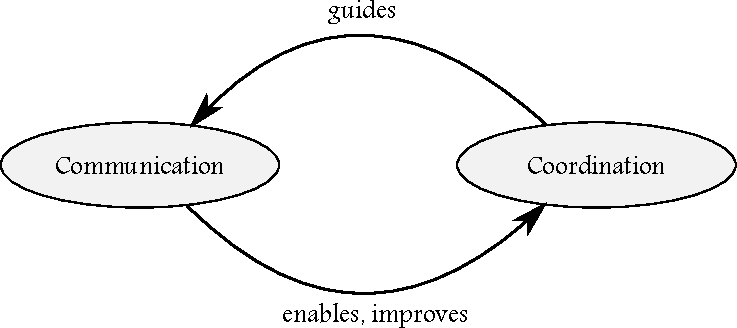
\includegraphics[scale=1.0]{commcoord}
\caption{\label{fig:CommCoord}Intertwined coordination and communication.}
\end{figure}


\subsection{The Centrality of the Coordination and Communication Problem}
\label{sec:Centrality}

The previous discussion should be sufficient to support the claim that coordination and communication are prevalent activities in collaborative software development. However, we can go further: an analysis of the commonly accepted problems and risks in software development projects leads us to conclude that coordination and communication are, nowadays, the central problem of software development.

The most widely known argument on the essential difficulties of software development is Brooks' ``No Silver Bullet'' essay \shortcite{Brooks1986}, in which he writes:

\begin{quote}
\emph{The essence of a software entity is a construct of interlocking concepts. [...] I believe the hard part of building software to be the specification, design, and testing of this conceptual construct, not the labor of representing it and testing the fidelity of the representation.}
\end{quote}

Thus even developing software in solitary and for personal use is fraught with difficulties. But as Brooks \shortcite{Brooks1975} himself discussed, this essential difficulty of software development, this struggle to capture the interlocking conceptual complexities of a software entity, is amplified significantly when software is developed in collaboration and for use by others. Not only is it difficult to specify the conceptual constructs that need to be eventually represented and tested, but the specification necessarily assumes some implicit knowledge that must be shared by numerous members of the development team. Not only does the design of these constructs need to fit harmoniously with the socio-technical systems in which they will be used, but several people in the design team need to learn enough about those socio-technical systems and ensure that their implementation strategy is easily accessible to people without their deeper domain expertise. Developers deal with problems and solutions so large and complex that nobody can know everything about them: the necessary information and judgment for a task often lies, at least partially, with someone else. In other words, the need to coordinate and communicate magnifies the essential difficulties of software development.

There are manifestations of this problem in many of the subdisciplines of our field, which are arguably about coordination and communication under a different guise. For instance, the entire ``requirements engineering'' literature is an effort to address the problems of communicating enough knowledge about a domain and about the implementation of a solution for that domain to a group of developers, of documenting such potential solutions reliably, and of coordinating changes to those solutions efficiently.

And while requirements errors are the most expensive errors in software projects \cite{Boehm1981}, in projects with traditional development lifecycles integration errors are just as problematic: it is in the integration phase that breakdowns in coordination and communication finally become apparent in the form of mismatching interfaces, incompatibility between modules, and inadequate testing.\footnote{\textbf{Microsoft:} Brooks stated that these problems increase significantly with the size of the development team, but it is difficult to understand the scale of the problem without analyzing it firsthand. As an example, in our Microsoft Study, the sample of ten bugs I studied included one case where 42 people coordinated to solve the problem and nearly three hundred people more received some communication about it. Two other bugs involved about two dozens of people coordinating to solve them. The single feature development case of that study uncovered the direct involvement of 45 people and the indirect involvement of 23 more in its design or implementation, and the creation of 21 documents spanning hundreds of pages, all of this for the addition of a checkbox in a widely used software product. The study also discovered the use of highly inefficient (though perhaps necessary) coordination patterns, such as the firing off of emails to hundreds of unknown recipients in the hope that one of them, somewhere, can provide some expertise in the resolution of the problem. This list of coordination patterns can be found in tables \ref{tab:MicrosoftPatterns1} and \ref{tab:MicrosoftPatterns2}. The challenge of coordinating the resolution of integration errors in the smaller organizations of my case studies was comparably far simpler.}

These requirements and integration challenges should be compared with the purely technical problems that software teams struggle with. The profession of software development continues to demand a high degree of technical sophistication, and there are many highly complex problems that reach the limits of our Computer Science knowledge. However, the great majority of our software projects take place completely or mostly within the bounds of such knowledge. For these projects technical challenges are certainly present, but the effort that they demand is overshadowed (and magnified) by the coordination and communication effort.\footnote{\textbf{Scientific Groups, Particle Physics:} Even projects that one might think are pushing the boundaries sometimes turn out to have fairly typical software development challenges. The ATLAS project probes questions at the very edge of our knowledge of the Universe, and yet the five participants of this project that I interviewed seemed most blocked by questions regarding the use and modification of the ATLAS software: how to get it to run under certain conditions, how to extract the data they need, what happens if they modify a certain piece of code. Their supervisors expect them to struggle with these questions for at least one or two years. To ease their learning process, these scientific groups resort to establishing liaisons to the headquarters of the project at CERN or to other research centres through postdoctoral fellowships or research visits: a visiting postdoctoral fellow is a source of knowledge about the intricacies of the ATLAS software. I only observed this dynamic in two cases: the ATLAS project and a medium-scale protein-interaction project.}

In sum, coordination and communication problems amplify the essential difficulties inherent in software development. Considering their prevalence, they are the central problems of our field.


\subsection{The Difficulty of the Coordination and Communication Problem}

Having established that effective coordination and communication is the central problem of software development, I will now show that it is particularly difficult to achieve due to the overwhelming amount of information that group members need to parse, the need for the development of tacit, complex, and specialized knowledge, and the exploratory nature of many software projects.

First, it should be well known that non-trivial software projects produce an overwhelming amount of information \cite{Yatani2009}.\footnote{\textbf{Microsoft:} Recall that three out of the ten cases in this study of bug fixing included more than one hundred interaction events. No comparable metrics were collected in the rest of my studies.} Group members who want to stay informed of every event in their team would need to dedicate so much time to reading the code, the emails, the bug database entries, version control logs, specifications, design documents, and other artifacts that their teammates produce that they may not have any time left to produce information of their own. Furthermore, researchers and software professionals continue to create tools to generate and transmit even more information on the grounds that it is to the advantage of the software team to have access to it.

This abundance of information translates into a scarcity of attention. Each group member makes their own decisions as to what pieces of information they will invest their time with, and these decisions are based on their own personal perspective of what are the priorities and the activities that matter for their group. Facilitating these decisions is one of the main challenges of knowledge management \cite{Alavi2001}, and it is the source of much promising work in our field \cite{Treude2009}, but our current solutions only ameliorate the problem.

The problem of coordination and communication, however, is deeper than one of a simple abundance of information to parse. Members of software organizations often need to develop tacit, complex, and specialized knowledge \cite{Schon1984}, of a kind which is unfeasible to document or operationalize.\footnote{\textbf{Contrast, Bespoker:} This was one of the principal reasons for the reluctance of Bespoker to engage in outsourcing development. The members of the organization did not think that they could successfully associate with a team from a different country and, therefore, a different context. When the organization was forced to offshore part of its development to keep a major contract, the project manager took exhaustive care to ensure that the offshore developers in India understood some details of North American policy (the domain of the application); the two firms also established a project liaison to be sitting in Bespoker's offices to relay missing pieces of tacit information as they become apparent, among other things. This example is one of many observed instances of people explicitly making an effort to overcome problems caused by the unavailability of tacit and complex knowledge; see section \ref{sec:Spreading} for more examples.} The need to develop this knowledge is evident in reports of acclimatization of newcomers to a software organization \cite{Sim1998,Begel2008},\footnote{\textbf{Contrast, Saville:} This firm has developed several strategies to speed up the acclimatization of newcomers. All software development happens in large communal rooms (more on that later), and all the current development tasks are visible for the whole group to see. Every morning, each team has a ``stand-up meeting,'' lasting somewhere between five and twenty minutes, where they discuss the events of the previous day and state what they intend to do now. Most code is developed in pairs, and the pairs are constantly shuffled so that most team members know about the structure, architecture, and ``tricks'' of all the relevant modules in the code. Organization members repeatedly refer to this process as ``spreading the knowledge.'' No other organization in my case studies had this kind of proactive effort to share tacit knowledge among its members.} but acclimatized developers still need to maintain it, and failure to do so has been found to be a major source of project falure \cite{Herbsleb1999}.

This means, in practice, that it is not enough to have access to a piece of information; one needs to understand enough of its context and of its implicit assumptions to make sense of it, and knowledge of its context and of its implicit assumptions cannot be achieved without effort and practice. A requirements document is rarely fully comprehensible on its own,\footnote{\textbf{Contrast, Bespoker:} Requirements documents do not usually seem to be intended to be comprehensible on their own, nor are they assumed to hold all important knowledge about the requirements of their projects. In the project with an offshore component, a business analyst in the team had been documenting, with significant detail, the requirements of the project; the project manager briefed the offshore team extensively on the nature of the domain of the project, on the architecture and design decisions of its finished components, and so on. Still, used to co-located development, the project manager was anxious about the success of the project and the coordination and communication demands of distributed software development, and decided to assign the India team a component of the new system that was as autonomous and disconnected from the rest as possible. In most of the cases that I studied, requirements documents (if they existed) were meant to be interpreted with assistance from their writers.} designers like to walk around the office to get a sense of the situation of their team \cite{Bellotti1996}, and Beck \shortcite{Beck1999} recommends to have a customer on-site, and the full development team sitting together, to increase the availability of implicit knowledge to the team.

Finally, to complicate things further, much software development has an exploratory nature. The problem domain and the solution may not be clear throughout most of the project, and software development becomes a creative and a discovery activity. Obstacles may arise anywhere, unpredictably, and this increases the need (and the difficulty) of establishing swift, trustworthy dynamics to communicate immediate and foreseeable problems and to coordinate to address them. In other words, the challenge that organization members face is not only one of uncertainty, but of equivocality \cite{Daft1986}: not only is there an absence of information, but there are multiple and conflicting interpretations about the situation of the organization.

Although there does not seem to be a solution that can tackle the tripartite problem of scarcity of attention, development of tacit knowledge, and equivocality, some tools or practices provide gains in some of these areas. In particular, for many of the events that matter in software development, effective coordination and communication cannot be reliably achieved through the simple transfer of data between people and artifacts.\footnote{\textbf{Microsoft:} Many of the problems and missteps we documented in the Microsoft study consisted precisely of a failure to coordinate and communicate through a simple transfer of data. At some Microsoft divisions build failures generate automatic bug reports with a wealth of data describing the failure, but such bug reports are considered by the relevant developers as merely the first set of hints to understand the problem. Typically, a discussion between several developers that try to resolve the issue ensues after such a bug report. For instance, for a particularly troubling bug, one that occasionally appeared in automated testing but could not be reproduced, and that was threatening to delay the release of a product, spurred several developers and project managers to share all the information they had about it, and to try to make sense of it. After much deduction, the problem was eventually linked to an error in the automated testing environment. The other case studies offer similar, ample evidence of the inadequacy of the simple transfer of data for the purpose of coordination and communication: the ATLAS researchers complained of such an abundance of documentation that they did not know what to pay attention to; IBM required frequent release meetings to make sense of the status of the modules of their products, beyond the information they would get in their dashboards; and Bespoker could not rely on requirements documents as its sole communication mechanism for offshore development.} A deeper, \emph{shared understanding} of the situation among its participants needs to take place. The next section discusses this concept.


\subsection{Easterbrook's Shared Understanding}

For this exposition of the concept of shared understanding I follow loosely Easterbrook's \shortcite{Easterbrook1994} unpublished manuscript on the topic, although whereas Easterbrook concludes with an interpersonal theory of shared understanding, I focus on an organizational use of the concept. Since Easterbrook's manuscript is not publicly available I will delineate some of its central points here.

Easterbrook points out that software teams must develop an understanding of the system and its context, and that this understanding is likely derived from fragmentary information because it is obtained through interaction ``with a number of disparate communities.'' He stresses that this understanding needs to be shared with the team, and that it will not be captured in technical documentation, since documentation, as I discussed earlier, ``will not include informal, anecdotal, or intangible information. (...) At the most, we can expect such documentation to provide a kind of anchor for the analysts' understanding.''

The term \emph{shared understanding} had been previously mentioned in the software literature. For instance, Walz \shortcite{Walz1993} reports on the development of shared understanding in a design team. However, as Easterbrook points out, the term is used freely and it is rarely defined. For his definition, Easterbrook uses constructs from the cognitivist study of mental models \cite{Rogers1992}, and emphasizes that individual mental models are partial, potentially inconsistent, and as superficial as they can be. As a result, ``mental models allow participants to derive a number of expectations about a situation, which they use both to explain the situation, and to make predictions. However, these expectations are often not borne out. A \emph{co-ordination breakdown}\footnote{The concept of \emph{breakdown} here is related to the breakdowns in tool use as discussed by Winograd and Flores \shortcite{Winograd1986} and Heidegger's \shortcite{Heidegger1927} \emph{ready-at-hand} concept.} is a mismatch between the expectations of one participant and the actions of another. The event that causes the breakdown may be a communication act. The mismatch might be the result of an error of communication or of perception by either party, or a difference in understanding of the situation. However, the existence of any of these conditions will not necessarily lead to breakdown.''

Using these elements, Easterbrook defines shared understanding as follows:

\begin{quote}
\emph{Two or more participants have a shared understanding of some situation, if the elements of their mental models salient to that situation are functionally equivalent. By functional equivalence, we mean that the models will provide the same explanations and the same predictions of a situation.}
\end{quote}

He explains that the relationship of shared understanding to situation is crucial (since it focalizes the concept to a meaningful and achievable scope). He uses the term \emph{situation} as ``an episode of interaction and the environment in which it takes place.'' \cite{Cody1985}. Furthermore, he differentiates between \emph{fragile} and \emph{robust} shared understanding, ``depending on whether it still holds in different situations.''

Easterbrook states that for any situation, the elements of the mental models of the participants can either be equivalent (in which case participants have a shared understanding), complementary (in which case participants have different, but not conflicting, perspectives on a situation) or conflicting (in which case they generate inconsistent expectations). Over time, the mental models and the relationship between them changes, as Figure \ref{EasterbrookSUDynamicsFig} shows. Models go through transitions of specialization and sharing, and of breakdown and harmonization; the two sets of transitions are orthogonal to each other. Easterbrook claims that breakdown dynamics, though usually seen as symptomatic of dysfunctional teams, are not necessarily negative: there are some cases in which a team may want to probe the limits or correctness of its shared understanding, and conflict may teach an organization important lessons about its systems and context. Finally, Easterbrook lists some mechanisms and techniques to bring about a shared understanding or a breakdown in groups of people in order to exploit his theory. The arguments in the remainder of this thesis are indebted to his discussion on the topic.

\begin{figure}[tb]
\centering
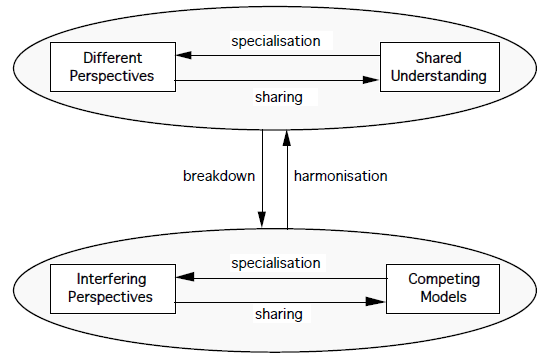
\includegraphics[scale=0.7]{sme-su}
\caption{\label{EasterbrookSUDynamicsFig}Easterbrook's transitions between sets of mental models.}
\end{figure}



\section{The Argument for Shared Understanding}
\label{sec:Argument}
\label{sec:SUTheory}


At this point we are ready to merge the threads of coordination, communication, and shared understanding into a cohesive structure. In this chapter I have argued that coordination and communication are central problems of software development, and that their main difficulties spawn from the overwhelming amount of information that organization members need to parse, from the need to develop tacit, complex, and specialized knowledge, and from the exploratory and creative nature of software development. For many of the events that matter in software development, effective coordination and communication cannot be reliably achieved through the simple transfer of data among people and between people and artifacts: a deeper understanding of the situations in which an organization acts, and of the strategies that the organization will deploy, must be shared by its members.

In this sense, the definitions of coordination and communication that I provided in the Introduction are unsatisfactory: they do not point to the particular difficulties of coordination and communication in software development (or, generally, in any intellectually-demanding, exploratory, collaborative task).

I propose that the concept of shared understanding, as defined in the previous section, can be profitably used to describe the coordination and communication constructs. The corresponding definitions are the following:

\begin{quote}
\emph{\textbf{Coordination} among participants in a situation consists of sharing and negotiating an understanding of their goals and plans.}
\end{quote}
 
\begin{quote}
\emph{\textbf{Communication} among participants in a situation consists of sharing an understanding of their status and context.}
\end{quote}

These definitions link the intertwined concepts of coordination and communication: both consist of the development of shared understanding among members of the organization. The distinction lies in the nature of the things that need to be shared: goals and plans for the purpose of coordination; status and context for communication. The reader should remember that this shared understanding is situation-based, as discussed in the previous section. \emph{Goals}, in this context, are what participants wish to achieve as a result of the situation. \emph{Plans} are the set of decisions and actions to be taken to address the situation. \emph{Status} consists of the current characteristics of the elements of the situation, and \emph{context} consists of the characteristics of surrounding elements that may have a bearing on the situation. In this sense, the conjunction of status and context consists of \emph{all} the information, implicit or explicit, that is accessible to the participants of the situation. The difference between status and context is that status corresponds to those elements that participants recognize to be central to the situation, while context corresponds to elements that are peripheral (and perhaps irrelevant) to the situation.

These definitions are both \emph{general} and \emph{discriminating}. That is, they are flexible enough to fit all attempts of communication and coordination phenomena as usually understood in our domain, but they give greater value to those attempts that address the challenges of coordination and communication effectively by being \emph{synchronous}, \emph{proximate}, \emph{proportionate}, and \emph{mature}, as these characteristics simplify the development of a shared understanding. Figure \ref{fig:Schema} summarizes these points, and the following paragraphs explain the four attributes of interaction.

\begin{figure}[tb]
\centering
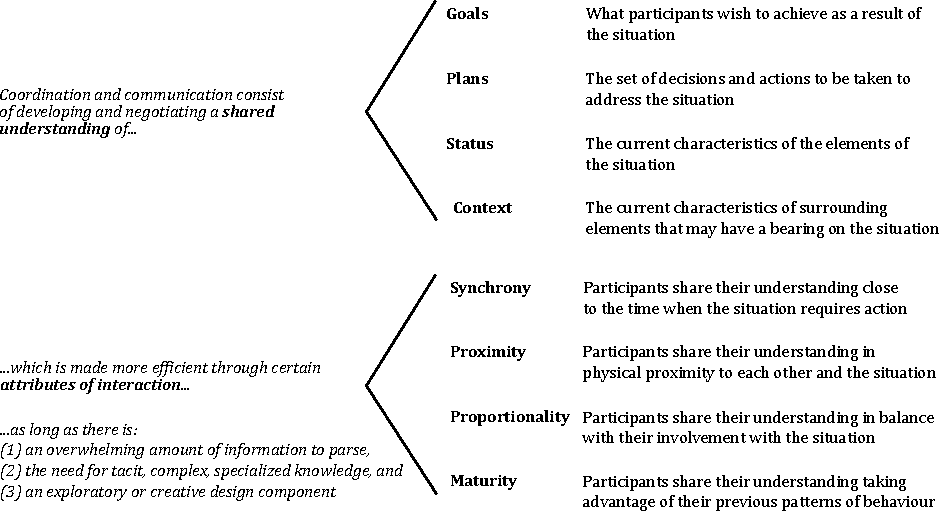
\includegraphics[scale=1.0]{su-schema}
\caption{\label{fig:Schema}The elements of shared understanding.}
\end{figure}



\subsection{Synchrony}

Our conceptualization of shared understanding makes explicit the fact that it is situation-dependent. It does not make sense to talk about a comprehensive shared understanding among the complete mental models of several people: such understanding is theoretically impossible (it demands an exact replica of the same mental model across all the agents involved) and empirically non-demonstrable. We can talk, however, about shared understanding as it relates to a specific situation, and about the fragility or robustness of this understanding depending on whether it holds under several situations.

Although there can be some ``carry over'' from previous situations, a shared understanding needs to be developed on a situation-by-situation basis. However, in an exploratory, creative activity such as software development, many situations are unforeseeable, and in many cases the scope of the foreseeable and probable situations is too large to be manageable. In practice, we resort to modifying our plans, prospects, and behaviour in response to the characteristics of the situations we encounter \cite{Suchman1987}.

This implies that an understanding that is shared \emph{synchronously} to the situation in which it applies is more effective than an understanding about multiple potential situations shared asynchronously, in advance.\footnote{This distinction is very similar to the coordination modes discussed by Van de Ven \emph{et al.}\ \shortcite{VanDeVen1976}. They distinguish between an impersonal, a personal, and a group mode of coordination. The first involves the establishment of rules, procedures, plans, and schedules. The second and third depend on feedback to make adjustments to the plans of action; March and Simon \shortcite{March1958} talk more generally about coordination by programming and coordination by feedback. Here I make the same distinction not only for coordination, but for communication as well.} Unless the domain and the possible consequences of our actions are exhaustively understood, preparing in full our plans and documenting in full our information before the relevant situations are encountered will be either inefficient (because we wasted much effort in describing all the possible avenues of action and all the possibly relevant implicit information) or simply unsuccessful (when we failed to prepare for the unexpected situation that in fact arose). Coordination and communication, then, are most effective when they take place in synchrony to the situations they address. This applies at all levels of activity.\footnote{\textbf{Contrast, Saville:} At a high level, Saville (and to a lesser extent Bespoker), in collaboration with the customer, selects the features to work on the next iteration at the end of the current one. This allows for flexibility in the direction of their systems, and for better feedback in terms of performance, quality, and customer satisfaction. At a low level, some teams at Saville have a ``daily priorities'' mini-meeting after their stand-up meeting. Lasting no more than three minutes, it consists of people stating what they plan to work on during the day, and who will they pair with. If the team leads do not think this is the best use of their time, they discuss alternatives until they reach something suitable together. Saville's tactics were the most synchronous of all the cases I studied.}

In other words, it is easier to share an understanding about a situation as it arises than to do so \emph{a priori}. In some cases, an \emph{ad hoc} shared understanding is unfeasible, and the organization needs to depend on plans and documents drawn in advance, but this does not mean that asynchronous strategies are superior to synchronous ones when there is a choice.

To clarify the convenience of synchrony, table \ref{tab:Synchrony} describes the difference between synchronous and asynchronous shared understanding for the elements of our coordination and communication constructs. 

\begin{table}[tbp]
\caption{\label{tab:Synchrony} Synchronous and asynchronous strategies}
\centering
\footnotesize{\begin{tabular}{p{2.0cm}p{5.8cm}p{5.8cm}}
\hline \hline
\vspace{1pt} \bfseries Shared understanding of... & \vspace{1pt} \bfseries Synchronous & \vspace{1pt} \bfseries Asynchronous \\
\hline
\vspace{0.5pt} Goals & \vspace{0.5pt} Takes advantage of a greater clarity of goals brought by the particulars of the situation. \par Example: Prioritizing the stories for an iteration at the end of the previous one. & \vspace{0.5pt} Implies a commitment to a specific set of goals when these are derived from partial and possibly incorrect information. \par Example: Charting the full set of desired features of a system during a requirements phase at the beginning of the project.\\
\hline
\vspace{0.5pt} Plans & \vspace{0.5pt} Can react to uncertainties flexibly; does not need to specify most decision branches. \par Example: Determining a list of daily priorities of the team in the morning, modifiable depending on context. & \vspace{0.5pt} Plans may need to be thrown away when more information becomes available, unless a significant effort is exerted to maintain them. \par Example: Committing the organization to the release of a fully specified set of features by a given date.\\
\hline
\vspace{0.5pt} Status & \vspace{0.5pt} Only a synchronous understanding of the status of a situation enables a truthful knowledge of its current state. \par Example: Learning what other team members are currently doing to decide what one needs to do next. & \vspace{0.5pt} There is no guarantee that the status of a situation days or months ago still holds, so asynchronous status sharing is highly uncertain. \par Example: Relying, halfway through a project, on original effort estimates to determine when the project will be finished.\\
\hline
\vspace{0.5pt} Context & \vspace{0.5pt} As with status, only a synchronous understanding of the context of a situation can highlight new, important, or surprising information. \par Example: Informing bug triaging decisions with knowledge of current priorities of the customers. & \vspace{0.5pt} There is no guarantee that the context of a situation days or months ago still holds, so asynchronous context sharing is highly uncertain. \par Example: Assuming that the customer's organizational structure and priorities are the same at project completion than at project inception.\\
\hline
\end{tabular}}
\end{table}

The examples in table \ref{tab:Synchrony} make it seem as if it were foolish to ever choose asynchronous strategies over synchronous strategies. This is not my intention. Certainly, and in particular when it comes to goal and plan setting, a broad understanding of the purpose of the organization's members and of their standard courses of action is quite healthy and beneficial. I discuss this in the Maturity section (\ref{sec:Maturity}) in greater depth. The argument advanced in this section is not opposed to guiding projects and organizations. Rather, the argument favours a flexibility of choice \emph{when such a thing is feasible}, so that decisions can be made when the facts are known.

In fact, under some circumstances, software organizations have little or no choice: they are required contractually to make plans asynchronously to the situations in which the plans will be executed, or they are only given some contextual information early on and are expected to make the most of it, or have such a large team that it is impossible to manage to coordinate them on a synchronous basis. In these cases, asynchronous strategies are called for. But according to my observations, asynchronous strategies are sometimes used when their synchronous counterparts would be easily applicable. Some software organizations, on the other hand, have managed to convince their customers of the advantages of synchrony, and therefore to change their customers' demands for asynchronous mechanisms.\footnote{\textbf{Small Firms, Agilista:} This firm only takes projects from customers that agree on synchronous, proximate mechanisms, as the firm's members do not want to work under other circumstances.
\par \textbf{Contrast, Saville:} This firm has managed to convince large financial and retail organizations, which typically demand a heavy asynchronous effort, to work in a relatively synchronous fashion. Some customers still demand documentation on an iteration basis, but since iterations are fairly short Saville has access to relatively fresh information to draw its goals and plans. Agilista and Saville were the only two cases I observed where the organization took active steps towards establishing a synchronous interaction with its customers.}

Finally, the table might give the impression that synchrony is a binary attribute: either an understanding is shared the moment the situation arises, or it is not. Synchrony, however, should be assessed with greater nuance. Year-old plans and week-old plans are both technically asynchronous, but they are not equally unreliable. Customer feedback that is an hour old is far more valuable than customer feedback months ago. The synchrony attribute, then, should be seen as a continuous dimension, where closeness to the present is desirable but rarely fully attainable.


\subsection{Proximity}

Since we are interested in a domain with large amounts of tacit information, developing a shared understanding is most effective when it occurs in physical proximity to its situation. This is because the richness and the opportunities provided by physical proximity are not matched by our current (nor by our potential) tools to collaborate at a distance \cite{Olson2000}.

In other words, if the agents that need to develop a shared understanding about a situation are physically proximate to the situation and to each other, they have access to a more significant portion of the tacit or implicit information that is necessary to a proper assimilation of the situation.\footnote{\textbf{Contrast:} An intense use of proximate strategies at Saville allowed me to get a quick understanding of the status of every team within the first day of my observations. Getting to the same level of understanding at Bespoker took a considerably longer time, and depended on numerous one-on-one interviews. I did not perform similar observations for the other case studies.} Unfortunately, we deal with an industry that increasingly focuses its activities in distributed development and offshoring, and some in our community advocate shutting developers in isolation in order to help them concentrate on their technical problems \cite{DeMarco1987}. And yet, as I have mentioned before, geographical distribution causes a greater number of coordination breakdowns \cite{Herbsleb1999}, physical co-location is a viable, effective strategy to improve the efficiency of software projects \cite{Teasley2002}, and many software development practices currently in use take advantage of physical proximity to share an understanding in a quick, reliable manner. Table \ref{tab:Proximity} specifies the differences between proximate and distant efforts to coordinate and communicate.

\begin{table}[tbp]
\caption{\label{tab:Proximity} Proximate and distant strategies}
\centering
\footnotesize{\begin{tabular}{p{2.0cm}p{5.8cm}p{5.8cm}}
\hline \hline
\vspace{1pt} \bfseries Shared understanding of... & \vspace{1pt} \bfseries Proximate & \vspace{1pt} \bfseries Distant \\
\hline
\vspace{0.5pt} Goals & \vspace{0.5pt} Implicit cues about a domain and a stakeholder become apparent when participants interact with them firsthand. \par Example: Picking non-verbal hints about a stakeholder's satisfaction in a product demo. & \vspace{0.5pt} Relies on explicit information to set and modify goals, with greater potential for breakdowns. \par Example: Using textual feedback from stakeholders to assess their satisfaction.\\
\hline
\vspace{0.5pt} Plans & \vspace{0.5pt} Can make use of team co-location to make plans easily shared and available. \par Example: Using whiteboards to track the components of stories that still need to be worked on. & \vspace{0.5pt} Must rely on poorer communication mechanisms to establish and update plans \par Example: Developing project plans for an offshore site.\\
\hline
\vspace{0.5pt} Status & \vspace{0.5pt} Implicit cues about the status of one's peers become apparent with direct interaction. \par Example: Daily stand-up meetings. & \vspace{0.5pt} Relies on explicit information to learn about the status of one's peers. \par Example: Management dashboards.\\
\hline
\vspace{0.5pt} Context & \vspace{0.5pt} Co-location shares details on many implicit contextual elements otherwise inaccessible. \par Example: The ``buzz'' or concentration of a pair of programmers that lets potential interruptors know when to ask a question. & \vspace{0.5pt} Implicit contextual details are often ignored. \par Example: Making a phone call to the same programmers to ask a question, while they were focused coding.\\
\hline
\end{tabular}}
\end{table}

As with the synchrony attribute, proximity is a continuous variable. However, it is not simply the plain distance between members of the organization that we are interested in: it is a matter of access and availability. The layout of one's office increases the saliency of some implicit details about one's peers, and hides others. A team could work in an open-plan room or in the same space with cubicles to very different effects. Doors, stairwells, and elevators have a disproportionate impact on the perceived availability of one's peers \cite{Allen1977}. And full proximity, or radical co-location, is not always possible, especially with larger organizations---although some, even among the largest, find ways to maintain most of the members of a team within physical reach from each other \cite{Bird2009}.\footnote{\textbf{Microsoft:} When interviewing people in this study, I found that it was common for me to find every one of the major players in the resultion of a bug in the same building---often in the same hallway. Even when this was not the case, the Microsoft campus has an extremely efficient system of shuttles to transport its workers quickly and on-demand between buildings. Several interviewees complained about Microsoft's relatively recent drive towards offshoring, as they could not just walk to the office of the offshore developers to sort things out. The other large organization I studied, IBM, did not have a comparable strategy to ensure proximity. Teleconferences were common at IBM, even among people working in the same building and across the hall.}


\subsection{Proportionality}

The concept of proportionality applied to coordination and communication is less common than those of synchrony and proximity, and it may require some explanation. Proportionality, in this context, refers to a balance between the involvement of each agent in the situation and the situation's needs; an alignment of responsibility with authority.

Proportionate coordination consists of coordination that is performed by the people who will be primarily affected by the consequences---and most knowledgeable about the details---of the situation they face. It emphasizes shared responsibility and team ownership of the strategies used to deal with the production of their systems.\footnote{\textbf{Contrast, Saville:} I witnessed a somewhat impressive proportionate coordination event in one of the teams of Saville. The team was behind schedule with a relatively new customer, and wished to convince the customer of its development style and performance. One day the team lead requested that everyone in the room analyzed the tasks that were pending for that iteration, and called for a meeting where they would decide if they were going to make it or not. At the meeting (and in the presence of their customer representative), he explained the pressure that the team was under from the customer's side. Team members spoke for or against the possibility of finishing their tasks on time. Although some people thought that it was manageable, it became clear that most believed it would not be: they had been overrunning their ambitious estimates in the past few weeks, and everything indicated that this would happen again. It was best, they said, to bring down the customer's expectations. To my surprise the team lead did not challenge the developers' opinions, and he did not try to force them into ``working harder'' to achieve their goals. He re-stated the emerging consensus and, somewhat resigned, said that he would communicate this to the customer and try to make the best of it. He did ask for the team to focus on finishing completely a fraction of the features so that the team had enough to show for the iteration. This event was unusual; I did not observe comparable situations in any other case study.} Proportionate coordination is also the principle behind self-organizing teams \cite{Moe2009}, and it is similar to Beck's \shortcite{Beck2005} concept of Accepted Responsibility:

\begin{quote}
\emph{Responsibility cannot be assigned; it can only be accepted. If someone tries to give you responsibility, only you can decide if you are responsible or if you aren't.}
\par \emph{The [Extreme Programming] practices reflect accepted responsibility by, for example, suggesting that whoever signs up to do work also estimates it. Similarly, the person responsible for implementing a story is ultimately responsible for the design, implementation, and testing of the story.}
\par \emph{With responsibility comes authority. Misalignments distort the team's communication. When a process expert can tell me how to work, but doesn't share in that work or its consequences, authority and responsibility are misaligned. Neither of us is in an intellectual position to see or use the feedback we need to improve. There is also an emotional cost of living with misalignment.}
\end{quote}

Disproportionate coordination is performed by people unrelated to the situation under consideration. It is an imposition of a plan of action and of the goals to pursue in the situation, determined by somebody other than those involved in it (usually by someone at a higher level in the corporate hierarchy) or by a mere fraction of those involved. According to my theory, the problem (beyond a loss of agency and the corresponding emotional cost that Beck speaks of) is that disproportionate coordination is inefficient: it consists of drawing plans without proper knowledge of the situation nor proper feedback from the execution of the plan, and it consists of setting goals that benefit only a fraction of the members of the organization. When high-level coordination is disproportionate, the goals of some members of the organization may be overlooked or dismissed. Under some circumstances this may lead to the successful completion of the software project from the point of view of those doing the coordination, but the same project may have been a failure from the point of view of those organization members that did not have a say in goal-setting and planning: they may have felt cheated by the organization and may leave when the opportunity arises. This loss of talent and experience is significantly harmful to the organization \cite{DeMarco1987}.

Proportionate communication, in turn, consists of enabling and allowing all the parties involved in a situation to share whatever knowledge they consider to be relevant to the resolution of their situation. It involves an open consultation with all stakeholders, and it prioritizes the feedback from those parties most knowledgeable and more directly affected by the situation. It is the foundation of strategies such as Participatory Design \cite{Kensing1998} and viewpoints-based modeling \cite{Easterbrook2005}.

Disproportionate communication, finally, relies only on information from a fraction of sources that leads to a picture of the situation that is incomplete in important ways. It does not seem as if there are any open advocates of disproportionate communication in the software research field, as its problems are evident, although disproportions in practice remain fairly common. Disproportionate coordination, however, has many advocates: it is the essence of many Process Engineering proposals (discussed in section \ref{sec:ProcessEngineering}). One of the reasons seems to be an understanding of software organizations as rational systems \cite{Scott2007}, a paradigm that is inadequate for the explorative, self-directed work in software organizations. It is more useful to conceive of software organizations as natural-open systems---that is, to treat them as ``collectivities whose participants are pursuing multiple interests, both disparate and common, but who recognize the value of perpetuating the organization as an important resource,'' collectivities that not only interact with their environment, but that have in this interaction an essential component to the viability of their system.\footnote{Chapter 3 discusses organizations as rational, natural, and open systems.}

Table \ref{tab:Proportionality} summarizes some of these observations regarding proportionality in our context. Note that proportionality, like synchrony and proximity, is not intended to be a binary dimension.

\begin{table}[tbp]
\caption{\label{tab:Proportionality} Proportionate and disproportionate strategies}
\centering
\footnotesize{\begin{tabular}{p{2.0cm}p{5.8cm}p{5.8cm}}
\hline \hline
\vspace{1pt} \bfseries Shared understanding of... & \vspace{1pt} \bfseries Proportionate & \vspace{1pt} \bfseries Disproportionate \\
\hline
\vspace{0.5pt} Goals & \vspace{0.5pt} The shared criteria for success are the result of negotiation between all stakeholders involved. \par Example: Decision making in self-organizing teams. & \vspace{0.5pt} Criteria for success benefit some stakeholders to the detriment of others. \par Example: Aggressive scheduling, project ``death marches.''\\
\hline
\vspace{0.5pt} Plans & \vspace{0.5pt} Those with most access to information get to plan the strategies to solve the situation. \par Example: Effort estimation performed by the developers who are going to write the corresponding code. & \vspace{0.5pt} Plans are prepared by people with partial knowledge and indirect feedback. \par Example: Effort estimation performed by managers or salespersons.\\
\hline
\vspace{0.5pt} Status & \vspace{0.5pt} The status of all participants in a situation is shared, and this information is weighted accordingly. \par Example: Customer involvement on-site, with developers probing the customer to understand project requirements. & \vspace{0.5pt} Status is shared selectively based on private agendas, or some participants are ignored. \par Example: Downplaying quality assurance reports to get a release out quickly.\\
\hline
\vspace{0.5pt} Context & \vspace{0.5pt} The full context of the situation is shared and weighted accordingly. Striving for teams of generalists rather than specialists. \par Example: Selecting programming pairs based on a mix of expertise of the code in which they will work. & \vspace{0.5pt} Context is shared on a (subjective) need-to-know basis. Favoring the formation of specialists and ``information hiding'' principles in the team. \par Example: Strong personal code ownership.\\
\hline
\end{tabular}}
\end{table}


\subsection{Maturity}
\label{sec:Maturity}

If every situation in software development was unique and unrelated to all others, it would not be necessary nor convenient to evolve patterns of responses to them. However, although each situation may be distinct from all others, it shares some patterns, a degree of similarity, to other situations encountered before. With each time that an organization faces a certain kind of situation, its reactions and expectations adapt, and it develops a vocabulary and a set of assumptions whose value lies in the fact that they arose from direct need.

In terms of shared understanding, this means that as an organization evolves its behaviour to face some particular kinds of situations, the difficulty of establishing a shared understanding of those kinds of situations decreases considerably. This is partially due to the internalization of tacit knowledge \cite{Schon1984}, and partially due to the establishment of a transactive memory system \cite{Wegner1991} that minimizes the coordination and communication requirements of the participants of a situation.

Interactions mature within the organization. Thus a process or practice that has been perfected in one organization cannot be formalized and simply ``copied'' to another one and assumed to work in the same manner.\footnote{The only example of a successful transplant of mature techniques that I found was the case of Saville, discussed below. However, it was initially problematic, and demanded a significant effort from all levels of the organization.} Pattern detection and familiarity occur within each organization member's mind (although progress done in other settings may be used profitably to simplify the adoption process and to share some common pitfalls and problems). Similarly, interactions mature out of need: maturity will develop in those areas of activity that are most often exercised.\footnote{\textbf{Microsoft:} The long list of steps that new features need to go through (including performance and security audits, test plans, and more) seem to be the result of an organizational learning that is more or less proven to work, and expected by all members of the organization. Similarly, the other large organization I studied, IBM, has a well established software development process and a division in charge of fine-tuning it according to the requirements of each of its groups.}

Therefore, organizations develop patterns of coordination and communication through their everyday experience. While the patterns of successful (or surviving) organizations are not necessarily optimal for their situation, they satisfice their goals, and we can at least assume them to be moderately efficient \cite{Aranda2007}. This means that, under many situations, the advantages of switching to a promising set of coordination and communication patterns has to be weighted against the loss in maturity entailed by engaging in a new (for the organization) set of coordination and communication patterns. Ultimately, then, this is an argument against radical changes in the management of software projects. Project managers cannot simply choose a new development method for their team and expect it to work well.\footnote{\textbf{Contrast, Saville:} As I describe in Appendix \ref{app:Contrast}, Saville did not begin as an Extreme Programming firm. When two senior developers convinced management to attempt a switch to agile practices, the effort mostly failed: some of the more technical practices (such as test-driven development) took some hold, but most did not. The firm eventually tried again, with the coaching of Kent Beck, and gradually established itself as an agile firm. Among possible success factors were the fact that the firm was already used to radical co-location, Beck's enthusiasm, a match between the Agile manifesto and the values of the firm's managers, and the willingness of the firm to learn a very different software development strategy, acknowledging the risks and early inefficiencies of the switch. Saville is the only case in my studies of an organization successfully making a significant change in its development strategy.}

Table \ref{tab:Maturity} clarifies the concept of maturity as it relates to coordination and communication patterns. Clearly, of course, maturity is also intended as a continuous variable.

\begin{table}[tbp]
\caption{\label{tab:Maturity} Mature and immature strategies}
\centering
\footnotesize{\begin{tabular}{p{2.0cm}p{5.8cm}p{5.8cm}}
\hline \hline
\vspace{1pt} \bfseries Shared understanding of... & \vspace{1pt} \bfseries Mature & \vspace{1pt} \bfseries Immature \\
\hline
\vspace{0.5pt} Goals & \vspace{0.5pt} Organization members know and (mostly) agree with their goals, and they can assume they are stable. They can make decisions on the spot in accordance to the organizational goals. \par Example: Team members relying on their previous behaviour to decide whether to postpone a defective release. & \vspace{0.5pt} No safe assumptions can be made about the goals of the organization or one's peers. \par Example: A group of university acquaintances creating a start-up for reasons unknown to each other. \\
\hline
\vspace{0.5pt} Plans & \vspace{0.5pt} In commonly encountered situations, participants know who is supposed to do what, and can react accordingly. \par Example: A developer that knows how a tester will test her module can leave ``hooks'' to simplify the tester's task, and the tester can expect they will be there. & \vspace{0.5pt} Participants remain highly uncertain about their peers' behaviour, and need to prepare more explicit plans for collaboration. \par Example: A newcomer to a project can at best be expected to do minimal contributions.\\
\hline
\vspace{0.5pt} Status & \vspace{0.5pt} The organization has found ways to share relevant status information quickly and efficiently. \par Example: Informative workspaces in agile team rooms. & \vspace{0.5pt} It is not clear what status information to share, or to whom. \par Example: Snowballing threads and shotgun emails (see table \ref{tab:MicrosoftPatterns1}).\\
\hline
\vspace{0.5pt} Context & \vspace{0.5pt} The members of the organization have learned which contextual pieces of information should be shared in many common situations. \par Example: Summarizing stories in one or two sentences in a story card. & \vspace{0.5pt} As many contextual pieces of information as possible need to be stated explicitly to strive for an appropriate shared understanding. \par Example: Thick, thoroughly specified requirements documents.\\
\hline
\end{tabular}}
\end{table}


\subsection{Summary of the argument}

The definitions of coordination and communication above help us discriminate among coordination and communication events and strategies that are more or less effective based on their fitness to the demands of our domain. The participants involved in a situation need to arrive to a state of shared understanding of their goals, plans, context, and status. As long as their situations involve an overwhelming amount of information to parse, tacit knowledge, and an exploratory or creative design component, this is easier to achieve if their strategies to share their understanding are synchronous, proximate, proportionate, and mature.

From this discussion we can conclude that organizations that have values, structures, and practices which facilitate the development of this shared understanding---strategies that adhere to the attributes discussed above---will find it easier to coordinate and communicate effectively, and that this ability will translate into greater success in their projects. Figure \ref{fig:Schema}, at the beginning of this section, puts these elements together.

It is important to note, however, that \emph{success} is dependent on the shared and the individual goals of the members of the organization and cannot be evaluated in isolation from these goals. Group members may wish to build a long-lasting organization, or to achieve a maximum profit from minimal effort, or to have a friendly, stress-free work environment, or to create products that advance the state of the art of their niche, or a variety of other possibilities. Furthermore, the goals of several group members may conflict with each other; an analysis of the degree of success of an organization has to consider the satisfaction of shared goals as well as the satisfaction of the personal goals of the people that conform the organization. This means that a broad and simple quantitative analysis of organizational success is unfeasible. I discuss this and other practical implications of this theory in Chapter 6.

For purposes of clarity, I present the main argument of this theory in point-form:

\begin{itemize}
\item Achieving effective coordination and communication is the central problem of software development.

\item Effective coordination and communication are particularly difficult to achieve due to (1) an overwhelming amount of information to parse, (2) the need for the development of tacit, complex, and specialized knowledge, and (3) the exploratory and creative nature of many software projects.

\item For many of the situations that matter, effective coordination and communication cannot be reliably achieved through the simple transfer of data between people and artifacts. A shared understanding of the goals, plans, status, and context among the participants of the situation needs to take place.

\item Although reaching a state of shared understanding is not easy, several characteristics of interaction contribute to its establishment. In particular, a shared understanding is reached more easily through the synchronous, proximate, proportionate, and mature interaction of the agents involved in the situation.

\item Organizations that have values, structures, and practices which facilitate the development of this shared understanding and its related attributes find it easier to coordinate and communicate effectively, and this ability translates into greater success in software development.
\end{itemize}

The argument simplified above is more than an academic distinction of the concepts of coordination and communication. As I will demonstrate shortly, the argument has several direct implications on constructs that are commonly used in software research and practice:

\begin{itemize}
\item Project lifecycle processes and documentation fare poorly from the point of view of the shared understanding attributes (synchrony, proximity, proportionality, and maturity). Their substitutes, however, often do not scale well, so project lifecycle processes and documentation may be necessary under some circumstances.

\item Practices and tools are valuable to the extent that they foster the shared understanding attributes, and they should be assessed under these criteria.

\item The appropriate use of physical space is a key strategy to enable synchrony and proximity directly, and proportionality and maturity indirectly.

\item Organizational growth hinders the use of effective but unscalable coordination and communication mechanisms, and it leads to the inefficient formalization of processes. Purely on these considerations, growth is harmful and it should be avoided.

\item Group cohesion enables the harmonious use of efficient coordination and communication strategies.

\end{itemize}

These implications are summarized in figure \ref{fig:Schema2}. The following section supports and explains these claims in detail.

\begin{figure}[tb]
\centering

\includegraphics[scale=1.0]{su-schema2}
\caption{\label{fig:Schema2}Implications of the theory.}
\end{figure}



\section{Implications}
\label{sec:Implications}

\subsection{Project Lifecycle Processes}

One of the most common constructs in software research is that of project lifecycle processes, also known as software development methods (or methodologies) and, more simply, processes. As I mentioned in section \ref{sec:ProcessEngineering}, designing lifecycle processes and their elements is an important component of the research agenda in this field, and development methods form the structural backbone of most current Software Engineering textbooks \cite{Pressman2004,Pfleeger2001,Ghezzi2003}.

This thesis uses the following definition of a project lifecycle process:

\begin{quote}
\emph{A \textbf{project lifecycle process} is the formalization of a repeatable, comprehensive, and generic plan to develop software projects.}
\end{quote}

The plan usually covers every major aspect of the life of the project, from inception to completion and beyond. It addresses questions such as how and who (which role) is going to elicit the requirements of the project, what should the team do if the customer wants to change a requirement, when and what does the team need to estimate effort, and what are the responsibilities of each role (and therefore of each individual).

The classic example of a project lifecycle process is the Waterfall Model, in which projects are expected to flow linearly and sequentially through a number of phases. The number and name of the phases changes, but includes elements such as Analysis, Design, Code, Test, and Maintenance.\footnote{Although Pressman \shortcite{Pressman2004} claims that the Waterfall Model ``remains a reasonable approach when requirements are well understood,'' and although much software research assumes its use, among the participants of my studies it seems to be nearly universally derided as lacking in sophistication and responsiveness.} Other common lifecycle processes are the Spiral Model and the Rational Unified Process.\footnote{I observed a variety of project lifecycle processes in use at different organizations in my case studies; I also recorded several organizations that did not follow any process at all. The following list is intended to provide a general background for the discussion in this section.
\par \textbf{Small Firms:} The cases in this study followed a variety of approaches to manage their software projects. Endosymbiotic used Scrum, Agilista followed XP, Spark followed no process at all, Bespoker used what seemed to be an adaptation of the Rational Unified Process (the picture, as I report in Appendix \ref{app:Contrast}, was more complex than that), PhoneOffshore implemented a loose waterfall with plenty of feedback loops, Growing Web's projects had generally too short a duration to warrant a full-fledged lifecycle process, and Rentcraft developed its products in iterations.
\par \textbf{Scientific Groups:} None of the cases in this study adopted a specific project lifecycle process.
\par \textbf{IBM:} An elaborate, extensible, and modifiable project lifecycle process is at the core of IBM's software development. Every group is responsible for providing a certain interface to other groups; internally they are free to pursue software development as they wish, within bounds, as long as the interfaces are satisfied and the goals met. Requirements for software projects are specified and prioritized years in advance, though there is much shuffling when projects get to their development phase.
\par \textbf{Microsoft:} As with IBM, projects are planned thoroughly. Each division pursues software development somewhat differently. Within a development cycle there are several milestones, in a spiral fashion.
\par \textbf{Contrast:} As described in Appendix \ref{app:Contrast}, I chose Bespoker and Saville because of their differences in project lifecycle processes. Bespoker, according to the Small Firms study, applied the Rational Unified Process, including the creation of detailed requirements documents and UML diagrams, and a small number of development iterations. Saville, in comparison, was a follower of Extreme Programming that was also experimenting with some proposals from Lean Manufacturing. Among other things this meant no requirements documents, many relatively short iterations, and tracking user requests through the use of a backlog and story cards. In reality, the picture was not as clear cut as this description, given to me by managers in both firms, would make it out to be. Appendix \ref{app:Contrast} has more details into the real approaches to project lifecycle processes in both organizations.} In comparison, some Agile ``processes'' (XP, Scrum) tend to provide only a very basic structure to the project, and therefore do not fall under my definition of project lifecycle processes. It is best to think of them as collections of practices, which I will discuss in section \ref{sec:Practices}.

In essence, a project lifecycle process prescribes the ideal (that is, unobstructed) workflow dynamics of a software organization. As such it is an attempt to coordinate software projects. It determines the groups and roles that will act on a project at any given time, the kinds of actions that they will take, and the people that they will pass their work to. Of course, this ideal prescription is rather abstract, so that not every detail is worked out, and it tends to be put aside when the process encounters an unexpected problem \cite{Suchman1987}. In terms of our theory, a project lifecycle process prescribes an \emph{asynchronous}, \emph{distant}, and \emph{disproportionate} approach to coordination. It is asynchronous and distant because plans are prescribed in advance, without real knowledge of the situations in which they will be applied.\footnote{Assuming, of course, that the corresponding situations do not fall under a predictable routine.} It is disproportionate because it is (usually) imposed by a number of people to a different or overlapping set of people. In other words, project lifecycle processes are an attempt to coordinate in advance, at a distance, and by decree.\footnote{\textbf{IBM:} The project lifecycle process followed by IBM has channels built in for grassroots modification, and at some level this modification is encouraged by the organization's higher management; an encouragement that should be seen as an attempt at proportionality. But such modifications are not straightforward: they must be approved by a process committee, and they must still adhere to the overall interfaces demanded by the process as is. I did not observe this mechanism at work in my other case studies.} Whoever makes the decision to use a lifecycle process determines that the rest of the organization will coordinate in the manner specified by the process to the extent possible, and that they will act in such a manner to achieve the particular goals that the lifecycle process chosen is meant to achieve. When the decision is announced to the organization, an understanding of the group's goals and plans is shared to its members. However, this understanding is imposed, rather than negotiated; other organization members have little choice but to quit or comply. It should be noted that in some cases, as with the higher levels of the Capability Maturity Model \cite{Humphrey1989}, a project lifecycle process is at least intended to \emph{mature} to suit the context of the organization.

The weaknesses discussed above should not lead us to conclude that these coordination efforts are always inferior and should be avoided. There are good reasons to engage in coordination through process definition and process adherence. First, if the process that an organization follows is formalized, then the organization can share this formalization to its members, and understanding the formalization allows them to make fair assumptions about areas of the organization that they are not familiar with. As time passes, this formalization is internalized, and thus, formalization allows for organizational growth and the coordination of larger groups of people. Second, as long as the organization members stick to the plan delineated in their lifecycle process, each of them can make better predictions of the actions and decisions of their team members. The organization becomes predictable to its members and a maturity of shared understanding of goals and plans arises, decreasing the possibility of breakdowns. In other words, established processes increase the \emph{maturity} of interactions in the organization.

Scalability and predictability are important factors for collaborative work, and therefore they are significant benefits of the formalization of project lifecycles. But this formalization also brings a number of problems. Some of them are caused by the nature of software development work: exploratory, creative, and complex. Our plans, our formalizations, are necessarily deficient: we cannot capture every detail and every exception in advance. And when the plans go wrong, when breakdowns occur (as they are bound to), a formalized organization does not have an efficient mechanism to recover; its members find themselves among strangers whose roles, skills, and habits they do not understand. The ``information hiding'' principle that enables effective formalization backfires under a breakdown.\footnote{\textbf{Microsoft:} We identified several pathological coordination patterns that were triggered by some discoveries of bugs or build errors. Microsoft employees would send emails to \emph{hundreds} of people, probing for information or expertise that could help them make sense of a new error. Most of the recipients had no way to help the sender of the emails, yet they would receive dozens of follow-up emails sent between the few developers with relevant expertise. In two of our cases the solution to the bug, discovered by a knowledgeable employee, was drowned under a stack of wild guesses; the knowledgeable person, a stranger to her peers, would have to try harder to be heard above the noise. This analysis was unique to the Microsoft study, so I do not have comparable information from other organizations.}

Even when things go well, project lifecycle plans sacrifice efficiency for repeatability and generality. Preset plans do not incorporate new information or project-specific characteristics (they are asynchronous and distant); if their execution is enforced at all times the result is highly specialized individuals spending their time performing process steps that are, often, clearly unnecessary.\footnote{\textbf{Microsoft:} Besides capturing information on ten bug cases, we tracked the development of a minor feature of a Microsoft product. This feature was minuscule when compared to the product that it was a part of; the project manager responsible for it stated repeatedly that it was so small that it could as well have been classified as a bug. However, since it was recorded as a feature, it triggered the whole feature development process of the division. It was assigned a software developer, a project manager, and a tester. It was also assigned, as secondary roles, a development owner, a user interface owner, a product planner, a test architecture reviewer, a security contact reviewer, three development reviewers, a technical writer, and contacts in other products, among other roles. It involved the creation of a summary specification, two functional specifications, two development design specifications, two test design specifications, two security risk assessments (all of these for two different milestones), a threat model document, a demo script document, legacy code removal tools, monitoring tools, and several hundreds of emails. Again, this analysis was unique to the Microsoft study; I do not have comparable information from other organizations.}

Furthermore, as I have discussed in section \ref{sec:ProcessEngineering}, a process-based approach to software development makes some questionable assumptions. It assumes that software development is a mechanistic activity with little need for discovery, design, creativity and exploration, and it assumes that the human element can be abstracted away from software research, an assumption taken to its most basic and alienating formulation by Osterweil's \shortcite{Osterweil1987} phrasing, ``software processes are software too.''

Most project lifecycle processes, therefore, are efforts to preestablish the plans, goals, and structures of an organization. Given the necessarily exploratory nature of software development, the uncertainties of the requirements, of the domain, and of the behaviour of project stakeholders and organization members, as well as the inefficiencies imposed by the push for repeatability and generality, they are far from an optimal solution.

As we will see, there are usually simpler, more adequate, and more informal solutions to the problem of effective coordination. However, these other solutions have dubious scalability. The one great advantage of a project lifecycle process approach is that it builds upon the natural inclination of organizations to formalize as they grow \cite{Blau1971,Haveman1993}. Therefore, if the members of an organization want to tackle projects of a great size, they must ensure their organization is large enough, and if it is not they must impose a level of process formalization on themselves as they grow. The difficulty resides in figuring the extent to which a formalization is made necessary by organizational size and structure, instead of misguidedly prescribed under the assumption that formalization leads to a more efficient coordination.



\subsection{Documentation}

Documentation, in the software development field, is tightly connected to project lifecycle processes: the release of documentation is often used to mark the progress of a project from a phase to the next, and the main building block of several project lifecycle processes is a document of some sort.

This thesis uses the following definition of documentation:

\begin{quote}
\emph{\textbf{Documentation} consists of text- or image-based artifacts created with the tripartite purpose of recording, communicating, and becoming enduring references for a piece of information relevant to a software project.}
\end{quote}

Most, and in some cases all, of the artifacts produced in software development projects are text- or image-based, but the previous definition is not meant to encompass all of them. Instead, it focuses on those that are created for the three reasons mentioned: to provide a \emph{record} of some project-relevant information, to attempt to \emph{communicate} said information through the sharing of the artifact, and to become a \emph{reference} for future activities in the project. Requirements documents, design documents, test plans, class diagrams, and sequence diagrams are examples of documentation using this definition, but code, emails, informal diagrams drawn on whiteboards, and story cards are not.\footnote{Some project artifacts lie in the borders of this definition. For instance, most mailing lists messages in open-source projects are not documentation, but a few may be written with the specific goals stated in the definition and are used as references for latter discussions in the mailing lists.}

The reputation of documentation-heavy approaches has suffered in recent years, and many software organizations of all kinds and sizes now advertise that they are ``agile'' and that they work with as little documentation as possible.\footnote{Recall that the Agile Manifesto signatories state that they value \emph{``working software over comprehensive documentation.''}} However, according to my observations, documentation is still heavily used in many software organizations, and even those most committed to agile principles resort to the use of documentation for a variety of reasons.\footnote{\textbf{Contrast, Saville:} This organization is strongly committed to the Agile Manifesto and to Extreme Programming in particular. However, all of its groups rely on documentation of one kind or another. Some documents are produced for contract negotiation, when necessary, and developers are sheltered from them to the extent possible. Other documents, such as ``wireframes'' (descriptions of the look and basic functionality of a screen), are widely used to give developers and customers an idea of the expected characteristics of the product. With the exception of the scientific groups, the other organizations I studied had an even greater reliance on some kinds of documents than Saville.} In particular, it seems that documentation is often present out of a need to establish a body of knowledge relevant to a project and to satisfy the demands of some customers, as a ``deliverable.''

From the perspective of the Shared Understanding theory, however, documentation is to communication what project lifecycle processes are to coordination. Documentation is a mechanism that attempts to communicate and establish a body of knowledge on a potentially large scale, to be used in a variety of situations. It is an attempt to reify the shared understanding of the team, so that the important pieces of information that the team members need to be aware of, and whose understanding they need to share, are captured in documents.

However, we know that documentation, generally speaking, cannot fully meet these goals, and in many projects it does a very poor job at them. I have discussed the issues with software documents before: first, they go stale quickly, since much of the information available when they are created becomes obsolete shortly afterwards; as reported by Lethbridge \emph{et al.}\ \shortcite{Lethbridge2003}, software developers tend to fail to update documentation.\footnote{\textbf{Contrast, Bespoker:} This is also the case for the teams at Bespoker that rely on documentation more intensely. Documents are produced on the early stages of a milestone or project, and they are not usually updated when their situation changes. However, this is not always the case: at Microsoft, feature development documents normally go through at least one revision in the course of their development.} Second, the people that should read the documents often do not read them \cite{Segal2005}; worse still, the creators of the documents assume that a silence on behalf of the supposed readers implies acceptance of the contents, not dread at the thought of ploughing through their thickness.\footnote{I discuss Lethbridge \emph{et al.}\ and Segal's studies in sections \ref{sec:Lethbridge} and \ref{sec:Segal} respectively.} And third, documentation cannot capture all of the necessary information relevant to a software team, since much of this information is tacit and needs to be learned through other mechanisms \cite{Schon1984}.\footnote{\textbf{Contrast:} This was the case both at Bespoker and Saville. In no case was the document itself sufficient as the only nor as the main tool for communication. Similarly, in my other studies, I found no major documents that were written with the intention of being a stand-alone communication artifact.}

Using the terms of our theory, documentation attempts to establish a shared understanding of the information relevant to software development situations \emph{asynchronously}, \emph{at a distance}, and \emph{disproportionately}. Its contents are often incorrect, incomplete, or superfluous to the situation at hand. For some purposes, this strategy may still be the best available alternative, and to some degree this appears to be the case at every project I have studied so far. The difficulty lies in determining when some documentation is necessary, and when is it inefficient and the information it intends to convey is better shared through some other mechanism. This is an important decision, considering the fact that the effort to create documentation is not trivial, and should not be thrown to waste.



\subsection{Practices}
\label{sec:Practices}

We can define a software practice as follows:

\begin{quote}
\emph{\textbf{Practices} are contained, repeatable, and transferable techniques used to improve some aspect of the performance of a software organization that is pertinent to the creation of its products.}
\end{quote}

It is possible to string together a set of complementary practices and to call the result a ``development process'' or ``method.'' Models like the CMM are supported by such sets of practices; the recent SEMAT initiative takes this position \cite{Jacobson2009}; and Extreme Programming is more akin to a set of practices than to a proper project lifecycle process. However, although they may synergize with others, software practices themselves are independent. Practices are mechanisms to attack a known software development problem, or to gain some generally useful benefit. They also give software organizations some low-level predictability, in the sense that its members know what to expect of their peers in commonly occurring situations.

Examples of software practices abound; they are popular constructs of our field, just as processes and documentation. For instance, \emph{code review} is a relatively well-researched practice to improve the quality of code; \emph{daily stand-up meetings} are used to provide status updates among team members and are a common occurrence of agile methods proposals; and \emph{Delphi estimations} are proposed to improve upon the individual efforts of software estimators by having them compare and iterate on their calculations.

Independently of their technical merits, however, these practices can and should be evaluated with respect to their consequences on establishing a robust shared understanding on software development organizations. A more detailed exploration of the above examples of software practices might make this emphasis on the development of shared understanding clearer.

First, let us consider \emph{code reviews}, which are prescribed mainly for their effect on software quality: they have been found to lead to greater error detection rates than traditional testing, at a lower cost \cite{Fagan1986}. There are many different kinds of code reviews, and some of them allow for very flexible steps and criteria, but the basic element of a code review is that a software developer submits a piece of code to a number of her peers, and they have the responsibility of analyzing the soundness of the code and of its underlying strategies, to spot defects and to provide recommendations for improvement. Some code reviews are performed face-to-face, some through software platforms. The number of reviewers varies; typically it goes from one to four, but larger groups are possible. Some organizations enforce the constraint that \emph{every} piece of code that enters their main repository has to pass a review; others only perform reviews selectively or upon request.

Proponents of code reviews argue that the technique effectively provides expert, or at least competent, attention and advice to the code produced by the organization, and that this attention uncovers logic errors and misunderstandings of the requirements that would be more difficult to detect through other software quality strategies \cite{Shull2002}. However, there are two other significant advantages to code reviews: they enable the \emph{reviewers} to learn about areas of the project that they might not otherwise explore, and they enable the \emph{group}, both authors and reviewers, to develop and enforce coding norms and styles.

To provide useful feedback, a reviewer needs to understand the purpose, architecture, and logic of the piece of code under review; once the review is over the author of the code leaves with a list of errors and the reviewer leaves with a better understanding of code created by someone else in the organization. If code reviews are widespread in the organization, one of their side effects is the build-up of group knowledge about all aspects of the code they work with. Effectively, reviewers emerge with a better understanding of the status and context of the code. Later on, if the reviewers need to modify or take ownership of any particular piece of code, they will know where to look for it and they will have an intuition of how it works. Traditional testing does not offer a similar benefit.

Additionally, a code review allows the whole team to interact more intensely, while focusing on the topic of code quality. They are now able to learn from each others' expertise, and if they want to pass inspections with minimal changes, they learn to write code in a way that adjusts to the team's style, idioms, and expectations. Over time, these interactions should lead to more mature coding norms and styles; Fagan \shortcite{Fagan1986} reports that developers who participate in inspections are less prone to introduce defects in their future work. Again, traditional testing offers nothing of the kind.

These are two instances of a practice leading to the development of a robust shared understanding in the organization that uses it. Although there is yet no empirical evidence of the impact of these factors in comparison to the direct impact in software quality, the mere observation that code inspections have these ``side effects'' leads to a reevaluation of the corresponding literature. For instance, Cohen \shortcite{Cohen2006} finds that increasing the number of reviewers in a code inspection quickly leads to diminishing returns from a defect detection point of view: the optimal number of reviewers is one. Similarly, Johnson and Tjahjono \shortcite{Johnson1998} find that code review meetings are not cost-effective, and Porter and Votta \shortcite{Porter1997} conclude that effort is driven primarily by the number of the reviewers participating in the inspection. However, from a shared understanding perspective a single reviewer is far from optimal, as the opportunities to establish a group culture and a group-wide understanding of as many pieces of the code as possible decrease significantly.\footnote{\textbf{Microsoft:} This was the case for one of the bug fixes I studied at Microsoft. One group had a policy to only accept code in their repository if it was reviewed by at least one person. Although in the case I analyzed this one-person review was reasonable (the fix involved importing code that solved the problem from a product built previously by the same group when they were working in another firm, one that was acquired by Microsoft along with its intellectual property, and everyone in the group were familiar with this code), in other cases a single reviewer would mean that most people would not be aware of important changes to the code. I did not observe cases of code reviews in my other studies.} To my knowledge there are yet no studies comparing the direct gains of decreasing the number of reviewers to maximize the ratio of defects-found-to-effort-spent against the indirect losses caused by a greater group ignorance of the work performed by peers and of their norms and expectations.

\emph{Daily stand-up meetings} are more obviously linked to the development of shared understanding: the team gets together and discusses the problems it found the day before and the plans for the day; evidently it is a coordination and communication activity, and it is prescribed for this reason \cite{Schwaber2001}. The one problem to keep in mind, however, is that the rote execution of the practice may not bring any of its intended benefits.\footnote{\textbf{Contrast, Saville:} In Saville there were daily stand-up meetings in every development team, and some of them were committed to the practice in letter and in spirit. However, several teams seemed to be executing the practice out of habit and of the expectation from team leaders that this is something to be done at this organization (in fact, high-ranking members of the organization believe that, though each team is relatively autonomous and free to choose its practices, there is the expectation that all teams have a daily stand-up meeting, and it would be an attack on the company's culture to do otherwise). In those less-than-enthusiastic teams, people would get together at a regular time, form a circle, and then, for the most part, have everyone ``pass'' on the opportunity to share yesterday's developments or the day's plans. There did not seem to be any direct or indirect benefit from such a half-hearted execution of the practice. I did not observe daily stand-up meetings in my other case studies.}

\emph{Delphi estimations}, finally, are meant to increase the accuracy of software estimators. This practice is not exclusive of software development; Boehm \shortcite{Boehm1981} popularized it in our field as follows: a number of experts are given a specification, they meet to discuss issues related to the specification, they estimate the effort to implement the specification separately and anonymously, a coordinator distributes a summary of the estimates, and the estimators meet again, discuss the divergences in the estimates, and prepare another round of estimation. The process is repeated until a consensus begins to arise.\footnote{\textbf{Contrast, Saville:} All user stories are estimated with an informal variant of the Delphi method. After a knowledgeable person shares the details of the user story to a group of three to five developers, they each give an estimate of the effort needed to finish each piece of the user story. The mechanism changes from team to team, but it usually involves everyone sticking out a number of fingers of their hands, representing the number of hours or ``story points'' required for that portion of the story. If there are notable differences in their estimates, they discuss their rationale until they come to a consensus. In my observations, this use of Delphi estimations was also unique to Saville: I did not record similar events at the other organizations I studied.}

By providing feedback to experts and the ability to discuss their perceptions of the specification among them, the Delphi method enables the synchronous, proximate, and proportionate development of shared understanding among them: their interaction leads them to a better grasp of the issues concerning the specification they are supposed to estimate, and differences in understanding provoke early and evident breakdowns and corresponding harmonization processes. As a result, the Delphi estimation method, independently of its advantages purely as an estimation technique, is at least in principle a valuable software practice from the point of view of our theory.

Given the variety of practices and of their motivations, it is not possible to claim that all of them help or hinder the establishment of a robust shared understanding. Some practices foster synchronous, proximal, proportionate, or mature dynamics, some do not. My claim here is that evaluating them with these criteria will give us a better sense of their worth.

In summary, the argument is that an organization can advance significantly on sharing an understanding through the judicious use of practices and without a larger and more restrictive project lifecycle process, \emph{as long as the practices can scale} to the number of participants that need to be kept involved in each situation. For the glaring problem of many practices in the literature is that they can only be executed by teams of modest sizes. Only the participating reviewers and authors gain any shared understanding benefits from a code review; only the participating attendants to a stand-up meeting gain any understanding from it; only the experts in a Delphi estimation gain a shared understanding of the specification. A large organization can ensure the execution of these practices in its sub-organizations, but any benefits gained from them will be as localized as the execution of the practices. Thus we see the need to formalize a software organization's processes as it grows: the practices that can sustain the development of shared understanding when the organization is small cannot sustain it as it grows.


\subsubsection{The Case of Extreme Programming}
\label{sec:Extreme}

Exploring the Extreme Programming proposal under this light is a useful exercise. There are two seminal books on Extreme Programming: the original work by Beck \shortcite{Beck1999} and his revision in a significantly modified second edition \cite{Beck2005}. As the second edition is more mature and has a greater clarity in the purpose of the prescriptions of Extreme Programming I use it as the focus of my discussion here.

For a proposal on software development techniques, Beck's Extreme Programming is an odd case. It emphasizes a perspective on organizational and personal values, on the humanity of software development, on communication, and on professional commitment to a work well done. One of its main points is that software development is much unlike assembly-line work; that it is a professional, almost artisanal pursuit, and that this is the essential insight of responsible software practice and needs to be taken to its extreme consequences.

Beck proposes a set of practices, but repeatedly claims that these practices will only work if the organization that executes them adheres to the organizational values that the XP framework upholds.\footnote{The values are Communication, Simplicity, Feedback, Courage, and Respect.} Linking these values to the practices are a number of principles, intermediate goals of the organization that are supposed to provide guidance to its members when it is not clear which practice to use or drop, or which decision to take.\footnote{The principles are Humanity, Economics, Mutual benefit, Self-similarity, Improvement, Diversity, Reflection, Flow, Opportunity, Redundancy, Failure, Quality, and ``Baby Steps.''} Robinson and Sharp \shortcite{Robinson2005} make a similar point, linking practices to values and explaining that what is important for an organization is to meet and uphold its values; the practices are simply instructions that work under some conditions to help the organization reach this goal.

From our point of view, what is striking is how much the practices of XP directly foster a development of shared understanding in a software organization; an effect I was able to observe firsthand at Saville in the Contrast study. The following is a brief description of the XP practices and their relationship to the development of shared understanding:

\begin{itemize}
\item \textbf{Sit together.} XP encourages radical team co-location \cite{Teasley2002}; arguing that having the full team sitting together enables teammates to develop a more robust group cohesion and awareness of the status, progress, and problems of each team member.\footnote{\textbf{Contrast, Saville:} All software development happens in team rooms with the same spatial layout: one large table in the centre with computers on its sides, all walls covered with whiteboards. People working in these rooms do not have a desk of their own; any personal belongings they want to have accessible during work hours are kept in personal lockers. In some teams people have eased into some spaces that are more or less their own, even though they are nominally shared; in other teams each individual shuffles around in different seats, sometimes three or four different seats in a single day. As a consequence, the status of the projects are immediately accessible to everyone. Customer demos take place in the same room, and when possible, a customer representative sits with the team throughout the duration of the whole project. Everyone knows if someone is sick or has a family emergency. Some employees are uncomfortable with this lack of privacy (hardly anyone checks their e-mail or browses websites during work hours), but most grow used to this and claim that it leads to stronger bonds with their peers. In my own experience, I was able to understand the context and status of their projects within the first day of sitting with the team---reaching the same state at Bespoker took a week and a half, and a number of one-on-one interviews. At other organizations, such as Microsoft and IBM, interviews were one of the few mechanisms by which I could reach a similar understanding of their projects.}

\item \textbf{Whole team.} Not only does XP propose that the full team should sit together, it considers as members of the team people that are usually relegated to the periphery of software development work: customers, managers, analysts, testers, etc. According to XP, all of these stakeholders should be immediately available to their peers, to the extent possible, so that as much of the knowledge necessary for the development of the software is spread among the team. None of the roles in the team is necessarily taken by one person; ideally, the best teams have no specialists.\footnote{\textbf{Contrast, Saville:} Except for administrative staff and the top tier of managers, everybody sits in the common team rooms. This includes customer representatives in two of the three divisions of Saville. Additionally, there seems to be an institutionalized aversion for specialization. People in all divisions spoke at several times of ``spreading the knowledge around,'' and one of the criteria to pair programmers was how much would one of the paired programmers learn about an area of the project she was not familiar with.
\par In one case, however, a developer told me that because of some carelessness he ended up being the only one in the organization that knew how to operate and modify a large-scale automated test suite. He explicitly said that he wanted to fix this, as the organization is opposed to ``silos.'' Among my cases, Saville's proactive push away from specialization was unique.}

\item \textbf{Informative workspace.} Given that the whole team is radically collocated, XP proposes to make the best use possible of its physical workspace through heavy use of whiteboards, story cards, and other props. These sensorial cues provide easily accessible information to the whole team \cite{Olson2000}, letting them know of the progress of their peers and of pieces of knowledge that are important to many of them.\footnote{\textbf{Contrast, Saville:} All teams followed the Informative workspace practice, and they provided me, visiting customers, managers, and developers, with numerous hints of the current state of the projects. The workspace was once specifically addressed in a group meeting. A manager stated that the fact that there were so many user stories mapped out in the whiteboards at various stages of completion meant that the team was spreading too much: they needed to focus on closing some of those stories as quickly as possible and free up the space. No other organization in my studies took advantage of their workspace in this manner.}

\item \textbf{Energized work and Slack.} Creative, productive work cannot be sustained over long periods for more than about 40 hours per week, nor under overly stressful conditions. These practices do not seem to have a direct impact on the development of shared understanding.\footnote{\textbf{Contrast, Saville:} They may, however, have some indirect benefits. At Saville, slack is encouraged, and it is normal to see people playing table tennis at all working hours and lingering in the lunch room while they play cards. This may help them establish and reinforce bonds with their peers, improving their cohesion, and go back to do focused work (and only focused work) in the team rooms. Other organization in my case studies, such as Bespoker and Microsoft, had similar approaches to slack and energized work.}

\item \textbf{Pair programming.} XP proposes that all production code should be developed in pairs: two people sitting in front of a single computer. Although the constant face-to-face interaction demanded by this practice causes some visceral reactions among solitary developers, and although pair programming has not been shown to bring direct productivity gains to the development team \cite{Arisholm2007}, the shared-understanding rationale to introduce pair programming to an organization is that much of the knowledge about every piece of code is shared by at least two members of the software organization.\footnote{\textbf{Contrast, Saville:} In several occasions, as mentioned above, developers would pair with the explicit goal of ``spreading the knowledge'' about a piece of code that a member of the pair was not familiar with. I documented no cases of pair programming in the rest of my case studies.}

\item \textbf{Stories.} Instead of capturing requirements in specification documents, XP uses the concept of ``stories'' and ``story cards;'' each relevant piece of functionality is captured in one or two relatively simple sentences written from the point of view of the customer. Stories are discarded once the corresponding functionality is implemented. This approach makes it far more likely that requirements will actually be read, known, and shared by the team and the customers, without introducing the overhead of writing and reading requirements documents.\footnote{\textbf{Contrast, Saville:} Furthermore, in most teams the stories are described, elaborated, and estimated by a team of four to six developers, at least one of whom will probably be involved in its development. I documented no cases of story definitions or of the use of story cards in the rest of my case studies.}

\item \textbf{Week cycle and quarterly cycle.} The actual length of the cycles varies depending on the context of the organization adopting XP and its customers, but in general XP projects progress with a short (1-3 weeks) and a long (2-6 months) iteration cycle. The shorter cycle provides the team immediate feedback on its progress and obstacles; the longer cycle gives the team and its customers an opportunity to take stock, reprioritize, and plan for the next iteration.

\item \textbf{Ten minute build, continuous integration, test-first programming, and incremental design.} These four practices are proposed with technical goals in mind, but they also have potential shared understanding benefits by simplifying the complexity of the build process (in the case of the ten minute build); providing immediate feedback on newly-created integration problems (continuous integration); allowing for the exploration of the requirements implicit in a story card by the creation of tests that, once the code passes them, will completely satisfy the story (test-first programming); and ensuring that the team is not committed to a design created early on, when the understanding of the domain is still probably low (incremental design).
\end{itemize}

In sum, an analysis of these practices and my evidence from the Saville case study show that one of the main goals of Extreme Programming is to enable the development of shared understanding in a software organization, explicitly in some cases and implicitly in others. Several practices directly aim to create an environment where the people involved in a situation can coordinate and communicate synchronously, proximally, proportionally, and maturely. To my knowledge this is the only software development proposal designed to address coordination and communication concerns so aggressively.

This analysis also shows that an organization that applies Extreme Programming both in letter and in spirit is a substantially different organization from the average software house. It works with different values, assumptions, and goals---it is a different organizational form \cite{Stinchcombe1965}. This point is confused both in the research and the trade literature by the legion of firms that claim to do agile development, or Extreme Programming, but that are far from committed to its philosophy and its organizational form.


\subsection{Tools}

The studies I reported in Chapter \ref{chap:Methods} did not have a tool development or tool evaluation component, so the following discussion is not based on my own empirical data, but on the reports from other researchers in the community. Beyond a short discussion on tool-enhanced coordination and communication, and pointers to the most promising research in the area, I have little to offer in this topic. However, at their core, tools have the same essential goals as practices, and we can use the same analytical principles in their study and design.

Software tools can be defined as follows:

\begin{quote}
\emph{\textbf{Software development tools} are electronic artifacts used to improve some aspect of the performance of a software organization that is pertinent to the creation of its products.}
\end{quote}

Tools, like practices, can be analyzed and evaluated from the perspective of the extent to which they foster or hinder the development of shared understanding in a software organization: whether they help members of the organization work synchronously, proximally, proportionally, and maturely. However, we find that many tools are built for developers working in solitary, and portraying a debugger or a compiler as shared understanding tools is inappropriate. Other tools are primarily used to coordinate or to communicate in a group: e-mail and instant messaging clients, portals, version control repositories, etc. Their use is so common among software (and other) organizations that advocating their use is not productive anymore.

There is a third kind of tools: those that are built for the purpose of coordination or communication, or that have some indirect impact on these goals, but whose use is not widespread, as they are still prototypes or unstable versions of potentially useful products. An example of this kind of tools, and arguably one that has already made the jump to widespread use, is \emph{Mylyn} \cite{Kersten2005}, which provides a task management interface on top of the Eclipse IDE, and which connects to commonly used repositories for tasks and bugs (Bugzilla, Trac, and JIRA). Other notable tools with a strong emphasis on coordination and communication are IBM's \emph{Jazz} \cite{Frost2007}, which emphasizes providing an awareness of every developer's activities and incorporates social tagging; Sarma's \emph{Tesseract} \cite{Sarma2009}, which attempts to reduce the problems of distributed software development through a dashboard with a geography- and activity-based set of panels; and Microsoft Research's \emph{Code Canvas} \cite{DeLine2010} and \emph{Codebook} \cite{Begel2010}, which respectively take advantage of our spatial awareness and of the socio-technical connections of the artifacts software developers use in order to improve their efficiency and performance.\footnote{\emph{Code Canvas}'s primary goal is not to simplify coordination or communication, but to provide a better sense of the interconnections between pieces of code and related documentation through a zooming mechanism. However, it includes some features for collaboration, so that people can ``enter'' the canvas of others, understand what they are currently working on, and leave artifacts prominently visible in the canvas for them to explore when they have the time.}

The challenge for several of these tools is to be able to filter out information that is irrelevant to their users in order to provide only what matters for the situation they currently face. The fact that we can build tools that give more and more information to members of software organizations does not mean that they will find it useful, and the poor speed with which some of these tools are adopted (and their abandonment after a trial period) suggests that the members of software organizations do not necessarily appreciate the wealth of data that these tools present to them. Distilling the essence of the questions that members of software organizations truly ask themselves \cite{Ko2007}, and then designing a tool that easily and effortlessly lets them find the answer to those questions, will probably lead to the greater advances in this area.


\subsection{Physical Space}

Much of the recent work on coordination and communication in software organizations has focused on overcoming the problems of distributed software development The push for offshoring development has made this kind of arrangement increasingly popular, even though it is known to be detrimental to the coordination and communication abilities of software teams \cite{Herbsleb1999}.

Less thought has been given to physical space layouts for teams working fully or mostly on the same site. Intuitively, we know that space and the distance and accessibility between members of a software team are factors that set the tone for their projects. Arrangements such as those of cubicle farms, or shared work rooms  encourage some kinds of interactions and disable others, although there still does not seem to be a consensus on optimal office space layouts for software development.

A popular argument claims that software organizations are most effective when they assign separate offices to each of their developers. The theoretical reason is that, since software development is cognitively complex and demanding, developers need to concentrate completely in their tasks, entering into a state of deep concentration named \emph{flow} \cite{Csikszentmihalyi1990}, an experience of full immersion, of harmony between one's actions, skills, and goals.  Since flow is both fragile and extremely important for successful creative activities, the argument goes, it needs to be nurtured in the organization by minimizing distractions. If developers are constantly being distracted at their workspace (by conversations, telephones, or the unpleasantness of smelling and listening to their peers' having lunch) they will never get anything done---and they will notice their failure, so that they will not only achieve nothing, they will become demoralized, leading to further failures in the future. Unfortunately, such distractions in co-located settings seem to be commonplace, and workflow is extremely fragmented \cite{Ko2007}.

The result of applying this argument to the design of office space is to maximize the ability of developers to isolate themselves if needed, under the reasoning that isolation leads to less interruptions and deeper concentration, which should lead to greater efficiency and product quality. Such an office space would provide every developer with a private office, even if it is relatively small, with a door that closes and a phone that can be silenced. Developers in this setting should not be expected to be online and available constantly throughout working hours, and the organization has to give them enough leeway to deal with their interruptions on their own time. When team interaction is necessary, developers should be able to use shared spaces, such as meeting rooms, and they should also have access to recreational space to socialize and recharge for their next bouts of concentration.

Proponents for this isolation often point to the popular book \emph{Peopleware} \cite{DeMarco1987}. Among other things, the book describes a competition among software developers implementing ``a series of benchmark coding and testing tasks in minimal time and with minimal defects.'' Participants record their time spent on a time log, and after they declare they are finished their products are subjected to a standard acceptance test. Developers work ``in their own work areas during normal work hours using the same languages, tools, terminals, and computers that they use for any other project.'' DeMarco and Lister found a considerable difference between competing individuals: the best participants outperformed the worst by a 10:1 ratio; the best one was 2.5 times better than the median; the better-than-median half outdid the worst-than-median half by a factor of 2. The differences could not be explained by the programming language, years of experience, salary, or number of defects submitted. The only strong predicting factor was where the participants worked: high performance competitors often came from the same companies, and their companies had better environmental factors than those of low performance competitors. Specifically, the better performers had more individual workspace, and their workspace was more quiet, private, and free of interruptions than that of the underperformers. DeMarco and Lister accept that this is not evidence of causality, merely of correlation, but claim that from a business perspective this should not matter: either a better workplace helps people perform better, or the people that perform better gravitate toward organizations that provide a better performance; the result of a good workplace is advantageous for these organizations no matter the rationale.

However, there is an important challenge to these results. DeMarco and Lister studied people working on a task \emph{individually}. To do well, participants had to work exclusively on their own to solve their problem in the best way possible. But in most cases software is not developed this way, as I discussed in section \ref{sec:Centrality}. Developers are part of a team, and the product of their individual work has to interact with that of many others; and they get and provide help to their peers. The coordination and communication demands that these teams face force us to consider alternatives to the maximal-isolation office layout derived from \emph{Peopleware}, under the assumption that an emphasis on coordination may be more important than an emphasis on concentration.

In fact, there are also theoretical reasons to emphasize coordination abilities. First of all, Csikszentmihalyi's theory of flow does not claim that flow happens exclusively in isolation---this is a misreading of the theory, which actually states that harmonious teamwork is one of the most accessible mechanisms to get into flow. Emphasizing coordination also brings other benefits. For instance, it enables the formation of the \emph{transactive memory systems} that I discussed in section \ref{sec:Transactive} \cite{Wegner1991,Hollingshead2000}.

Proximity also enables the use of richer communication channels: according to Olson and Olson, despite all our current technology for remote collaboration, face-to-face interaction is unsurpassed, and will continue to be decades from now, even if all of the reasonably feasible long-distance collaboration technologies materialize \cite{Olson2000}. Distributing people so that they are separated by a distance greater than a short walk decreases the chances that they will visit each other dramatically \cite{Allen1977}, which according to Olson and Olson leads to losses in rapid feedback, in nuance, and in implicit cues, among other problems. As mentioned in the discussion on Extreme Programming (section \ref{sec:Extreme}), agile proposals stress these points and suggest that the whole team should sit together in an informative workspace.

There is evidence that the inverse of a maximal-isolation approach, radical co-location, is beneficial to software organizations. I discussed some of this evidence, specifically the study of Teasley \emph{et al.}\ \shortcite{Teasley2002}, in section \ref{sec:Teasley}. They studied an automobile company that decided to try ``war rooms'' for their software development projects, first as a pilot program, and later for most of their development. The war rooms had a workstation for every project member, most of whom were sitting around a large desk, with whiteboards on the walls. There were also some private cubicles available nearby, outfitted with phones and computers, so team members could choose to go there if they needed silence and privacy.

The results were strongly in favour of the pilot teams: they outperformed their company baseline by a factor of two in terms of productivity, and though a few team members were uncomfortable with the arrangement, most of them liked the war rooms, grew comfortable with their more intense interaction, and preferred them over their old cubicles.\footnote{\textbf{Contrast, Saville:} The history of co-location in Saville is more accidental, but included the same pattern of growing comfortable with intense interaction and the accessibility of team members. Saville has had three main locations throughout its life. The first one was small and had offices distributed along a ``bowling alley'' hallway. The second was one large shared room. When Saville did no longer fit in this second office and started to plan the layout of the third, several members of the organization made the point that, whatever architectural layout the offices had, the team rooms aspect had to be preserved: they became used to having teammates nearby to collaborate more intensely, and did not want to return to their first layout. Saville's approach to the use of physical space was unique in my observations.} Subsequent teams, once the program had been institutionalized, had an even better performance, improving upon the pilot teams in all productivity metrics significantly while keeping the same degree of user and team satisfaction. Furthermore, interruptions in co-located environments do not seem to be as disruptive as those in isolated environments, according to Chong and Siino \shortcite{Chong2006}: the nature of the interruptions is different and more work-related, interruptions are shorter, and several contextual variables provide potential interruptors with hints regarding the best time to interrupt their targets causing minimal disruptions.

To my knowledge, no study has yet conciliated the contrasting results represented by DeMarco and Lister with those of Teasley \emph{et al.} However, the arguments in this thesis provide an explanation for their divergence. The explanation is based on a consideration of work patterns \cite{Tesluk1997}, as discussed in section \ref{sec:WorkPatterns}. Recall that we can classify workflow dynamics as belonging to one of four categories, from Pooled workflow (where the team aggregates individual performances without the need for interaction or exchange) to Intensive workflow (where work flows between all members of the group, potentially in any direction). The competition of DeMarco and Lister is an example of Pooled workflow, while the environment in Teasley \emph{et al.}'s study corresponds mostly to the Intensive workflow dynamic. This suggests that the intensity of the workflow of a team makes certain physical layouts more convenient than others.

The taxonomy, of course, is just an abstraction, and it is unlikely that teams will fall strictly in only one category. Generally speaking, however, software projects tend to fall in the last two levels, Reciprocal and Intensive, although the exact slot for any one team depends on the specific processes and practices that it uses. There are very few software projects for which the Pooled or Sequential patterns are feasible---pure waterfalls would be an example of sequential workflow, but nobody seems to be working with pure waterfalls. In comparison, the Reciprocal workflow pattern adjusts closely to real-life waterfall and spiral project lifecycles, while the Intensive workflow pattern matches agile strategies better. In other words, the more compartmentalized and formalized work is, the lesser the need to coordinate and communicate intensely. However, if such need is present, the team benefits from physical layouts that make it easier for them to reach a robust shared understanding.

This is because team co-location fosters all four shared understanding interaction attributes. It contributes directly to synchrony and proximity, for obvious reasons. But indirectly it also helps to improve proportionality, as participants become aware of more project situations and are able to intervene if necessary, and it helps to improve maturity, as their more frequent, intense interactions fall into observable and learnable patterns more quickly.

In sum, although the research on space layout for software organizations has presented conflicting findings, the framework in this thesis offers a viable explanation for their divergence. Physical layout should be consistent with the workflow patterns of the organization; the higher the demands for intensive workflow (that is, the greater the need for robust shared understanding), the greater the need for a radically co-located area that maximizes on-the-spot coordination.



\subsection{Organizational Growth}
\label{sec:SoftwareSize}

As I discussed in section \ref{sec:Size}, it is well known that increases in organizational size lead to greater bureaucracy and formalization \cite{Blau1971,Haveman1993} and to counter-productive organizational behaviours due to de-motivation \cite{Talacchi1960}. Organizational growth also leads to a loss in cohesion: all other things being equal, a small group develops a greater cohesion than a large group simply because day-to-day experiences allow for more interactions between every group member with respect to their potential total of possible interactions \cite{Homans1950}.

Despite the loss of cohesion in larger organizations, there are certain advantages to be gained from organizational growth. The actual advantages depend on the domain of the organization; three specific advantages in the domain of software development appear to be a better role specialization, greater power to release large products relatively quickly, and leveraging software features from complementary products owned by the same organization.

From the perspective of shared understanding, however, growth is problematic. It invalidates the applicability or the usefulness of some coordination and communication mechanisms: the team can no longer sit together in the same room, code reviews do not lead to an understanding of the full architecture of the team's project, awareness dashboards become unwieldy and mostly pointless at any level beyond that of small subteams of the organization. This leads to a need to formalize, to institute processes and documentation requirements, which we have discussed at the beginning of this section to be inefficient coordination and communication mechanisms.

If the members of an organization are committed to growth, but they intend to retain access to non-scalable mechanisms, an apparent solution lies in the formation of small teams within the larger organization. The members of these teams would not need to have a particularly strong relationship with their whole organization, but merely with their team mates; clusters of highly cohesive teams could be coordinated with a more formalized organizational skeleton to achieve organizational goals, while remaining sheltered from bureaucratization.\footnote{\textbf{Contrast:} This is more or less the strategy used by both Bespoker and Saville. Both organizations are divided in groups: Saville has three major divisions of roughly similar sizes; each division has a number of projects under development in the same broad area (for instance, Financial Services). Bespoker does not have a division-based structure, but every project has its own group. In both organizations, however, some people move around between groups and divisions as needed. The larger organizations I studied seemed to have a harder time to implement this strategy, as their (large) products are heavily dependent on each other.} This is an approach used with some success by the large players of the music industry \cite{Lopes1992}. But what works for music seems difficult to enforce and achieve in the software industry: every musical production is essentially separate from each other; its linkages to other works are artistic, not concrete. The giants of the software industry (Microsoft, IBM) are notorious for the interconnectedness of their products.\footnote{\textbf{IBM:} The amount of interconnections that release engineers and project managers need to keep straight is bewildering. The release team resorts to a gross simplification of the status of each group into a ``traffic light'' state: green, yellow, or red. The latter, of course, get all the attention in status meetings, but there is enough of them that even this attention is superficial, dealing with an abstracted representation of what the problems in the group are or might be.
\par \textbf{Microsoft:} It is known (and fought in court) that Microsoft's products are extremely interconnected. An instance of the negative side of this interconnection was the resolution of one of the bugs we investigated. The bug, which only appeared sporadically (within Microsoft these are called Heisenbugs) was initially reported in one product's bug database; after some investigation the team concluded that it was not responsible for it, and blamed a different Microsoft product. Bug ownership shifted in several occasions. Only after a joint meeting of high-ranking project managers of both products (what we in our table of coordination dynamics called a ``summit'') did the groups established a joint strategy to fix the bug. I did not observe similar challenges in my case studies of smaller organizations.} In these organizations, many teams depend on the products developed by many other teams; they must therefore define deadlines, requirements, and interfaces. The organizations are forced to create support teams whose task is to ensure compliance and improvement of the organization's processes. While it is certainly possible to isolate teams in a larger organization in order to create an environment of cohesion \cite{Teasley2002,Schwaber2001}, it is an effort that runs in opposition to the trends of most large software organizations, and it is not easily accomplished.

In contrast, the problem of small software organizations is that for many domains they can only tackle relatively small problems in acceptable times \cite{Brooks1975}. There are many opportunities that are out of reach for small groups; to reach them they must grow. This growth will make them less efficient per person, but the cumulative group efforts will allow them to accomplish more as a whole. The problems that lie in this path are, first, that the organization may grow to the point where its own survival and the hierarchical advancement of its members become the overarching goals of the organization's members, rather than the accomplishment of whatever purpose the organization originally meant to address \cite{Blau1971}; and second, that a later shrinkage of the organization will probably not result in a loss of formalization: though adding people to the organization almost certainly formalizes it and makes it more rigid and less cohesive, removing people does not necessarily lead to cohesion and flexibility, as the structures, processes, and behaviours of the older, larger organization continue to influence the activities of the newer and smaller group,\footnote{\textbf{Contrast, Bespoker:} At the time of my observations, Bespoker had gone through a significant downsizing of about 40\% of its staff, mainly caused by the economic downturn. This loss was not accompanied by a reduction in the amount or kind of formalization in most groups: the same documents and processes were expected as they had been in the past. The opportunity I had to observe the consequences of such a downsizing were unique to the Bespoker case, and I do not have comparable data from other organizations.} even, potentially, influencing the behaviour of new organizations formed from the remnants of the old.\footnote{\textbf{Contrast, Bespoker:} The process- and document-heavy approach to software development in some areas of Bespoker seems to be the result of its founders being familiar with this strategy from their earlier time as software consultants in a multinational. When they created a new firm, they continued to develop software in the same fashion. Only recently have they begun to ease up some of these processes and document requirements in some of their groups. The opportunity to observe this phenomenon, again, was in my case unique to Bespoker. I do not havd comparable data from other organizations.}



\subsection{Cohesion}

So far we have discussed several common concepts in the field of software research, and we have explored their advantages and disadvantages from the point of view of the shared understanding theory summarized in section \ref{sec:Argument}. There is another important concept regarding coordination, communication, and the shared understanding theory, but it is not usually addressed in software research studies. This is the concept of group cohesion, and we have observed some of its causes and consequences in our studies. Therefore it is useful to explore cohesion in some detail.

In section \ref{sec:Cohesion} I presented Festinger's \shortcite{Festinger1950} definition of cohesion as ``the resultant of all the forces acting on the members to remain in the group.''\footnote{That section also includes a discussion on the topic of cohesion in general.} I use a similar approach to cohesion in this work, and define it as follows:

\begin{quote}
\emph{\textbf{Cohesion} is the strength or intensity of the meaningful ties between members of a group.}
\end{quote}

We have seen how, for instance, project lifecycle processes and documentation are commonly accepted approaches to establish coordination and communication in software organizations. Cohesion, in contrast, is not usually thought of as a concept that has a similar impact in terms of coordination and communication---nor on any other terms except for group morale. However, group cohesion seems to be an enabler of conditions that foster effective coordination and communication mechanisms.

The reason is that many of the synchronous, proximate, proportionate, and mature mechanisms I have discussed up to this point appear to depend on a large extent on whether the members of the organization \emph{enjoy} working in close collaboration with their peers or not. If group cohesion is not present, either by personality conflicts or interpersonal frictions, then several of our proposals are in trouble: pair programming, self-organizing teams, radical co-location, and others.\footnote{As Greg Wilson told me in a personal communication, ``radical co-location is good, except that nobody likes to be radically co-located with an asshole.''} But if the members of the organization have a strong group cohesion, they are more familiar with each other's skills, weaknesses, preferences, working styles, implicit cues, vocabulary, and areas of specialization.

There appear to be some social characteristics that enable an easier or greater development of cohesion among members of organizations. Some are summarized in table \ref{tab:SmallFirmsDetails}. Among them we have observed:

\begin{itemize}
\item \textbf{Homophily.} A phenomenon that manifests as homogeneity in a social network, caused by a natural attraction of its members to similar individuals \cite{McPherson2001}.\footnote{\textbf{Small firms:} We found several instances of both status and value homophily in our cases (Agilista's shared engineering and professional background and PhoneOffshore's prevalence of employees of the same minority group, among others). Regarding the other case studies, Bespoker has a significant minority group seemingly banding together, and at Microsoft there is a large number of mailing lists and wikis created to appeal to a huge variety of needs and wants of the members of the organization.} This homogeneity may increase the efficiency and reliability of communication, and make it easier to develop a shared understanding of every aspect of the organization.

\item \textbf{Long-term collaborations.} Long-term relationships enable a deeper understanding of the work styles of one's colleagues, and a better estimation of their capabilities.\footnote{\textbf{Small firms:} Rentcraft's product manager and project leader duo had been working together through several companies over the years, Endosymbiotic's full team forked from a different company, Bespoker's partners had been collaborating through almost two decades. I observed similarly clear long-term collaborations among employees of Saville and of Microsoft.}

\item \textbf{Rejection of radical change.} For many organizations, their current practices have been negotiated, agreed, and settled in the past; they exhibit a large degree of organizational inertia \cite{Hannan1989}. Newcomers that intend to change processes significantly, or that do not accept established practices, may be received with hostility and may not last long.\footnote{\textbf{Small firms, Endosymbiotic:} This was the case with an employee who wanted to modify the practices of the group. In my other case studies, both attempted changes and rejection of those changes were less overt.}
\end{itemize}

Lastly, let us remember that cohesion, on its own, has been shown to improve team performance in many different settings \cite{Beal2003}. More importantly, my evidence and that of others shows that cohesive teams and organizations develop shared understanding without resorting to formalization \cite{Sharp2004,Chong2007,Teasley2002,Martin2007}, and that they take advantage of the exploratory, creative, and complex nature of software development more easily than teams and organizations that adopt a process- and documentation-heavy approach.\footnote{\textbf{Contrast:} This was the case at both firms. In Saville, instances of the phenomenon were commonplace. For instance, task assignment, which usually happened every day in the morning after stand-up meetings, was fast and full of implicit information on who is the most appropriate pair to tackle a problem (considering both the short-term efficiency of assigning the most knowledgeable people and the long-term efficiency of spreading the knowledge around); and when someone was transferred from one team to another, a team member would go over the main differences between how things were done in that team in comparison to the others in a matter of only a minute or so. In Bespoker, even though some projects supposedly relied on documents to communicate requirements and priorities, these were typically put away to explain this information in terms that team members would understand most easily. In both organizations there was at least one individual who, beside their nominal responsibilities, was recognized by most as a person holding the group together: someone well connected to the owners and that could hear about important obstacles or problems and be trusted to sort them out tactfully. I did not observe people playing a similar ``jelling'' role in the other organizations I studied, though DeMarco and Lister \shortcite{DeMarco1987} report on this phenomenon as well.}

One question related to group cohesion remains: once we recognize its value, how can we foster its development? Unfortunately, this thesis does not provide an answer to this question. An emphasis on homophily in recruitment processes may yield benefits in cohesion, but its inequality implications are problematic: the minorities in a largely homogeneous organization may be left out of some opportunities available to the majority. Another strategy, as Homans \shortcite{Homans1950} observed, is to promote the frequent interactions among people, as greater frequencies of interaction lead to a greater liking of one another. It is clear that some software organizations that are aware of the importance of cohesion take good care in bringing to their groups only people who seem to harmonize with them, but their strategies to achieve this, to date, are very much an art.\footnote{\textbf{Contrast:} Both Bespoker and Saville claim to take good care of hiring staff only if some fuzzy, subjective conditions are met. Bespoker, according to one of its founders, looks for people technically capable but friendly, unassuming, and easy-going; people they would enjoy spending time with in their pizza nights or in informal chit-chats. Saville employs several tactics in the interviewing process to assess the extent to which the potential recruit is comfortable in a high-context, intensely social work environment; these tactics have to do with body language when they give the candidate a tour of the team rooms, the candidate's recollections of past experiences, and the extent to which the candidate can make all interviewers feel included in their conversations.
\par The result in both cases is a healthy and positive work environment. Several people told me they were lucky to be working there, and that it was the best place they'd been. One made a comparison with IBM, where he used to work: he said that back then he could not wait to get out of his cubicle, every day; now he actually likes to go to work. Another told me that she had left the firm at one point for another opportunity that seemed better on paper and ``came running back.''
\par In my case, and on a very subjective note, after spending a mere three weeks at each of the firms I felt a genuine and touching openness in both of them. I played euchre, table tennis, poker (I lost \$10), and Rock Band; people welcomed me in their lunch tables, shared intimate details of their personal lives, praised my home-made salsas, and sincerely invited me to continue our relationship. Both were organizations where I could see myself working happily, had my path been different, and I was sad to leave them.}

\chapter{Discussion}

In the previous chapter I presented an argument that looks at coordination and communication as the central problem of current software development, and explained that coordination and communication cannot usefully be conceived in a simplistic manner in our domain. Instead, I presented a characterization based on the concept of shared understanding. I argued that coordination, effectively, consists of sharing an understanding about the goals and plans of the participants of the situation, and that communication, similarly, consists of sharing an understanding about the status and context of their situation. I then described several characteristics of interaction that enable or simplify the formation of shared understanding: synchrony, proximity, proportionality, and maturity. I argued that organizational strategies that foster these attributes lead to a more robust shared understanding, and therefore to more effective coordination and communication.

I then used this argument to revisit several common constructs in software research and explore the ways in which they are altered once we recognize the challenges of successful coordination and communication. Some of these constructs, such as processes, documentation, and organizational growth, are detrimental or ineffective to achieve coordination and communication; some others, such as some practices, tools, and the appropriate use of space, can be extremely valuable. It is not, I argued, that processes or documentation are simply \emph{wrong} or that practices and tools are \emph{right}. Rather, the problem is that processes and documentation tend to rely on ineffective mechanisms to coordinate or communicate, such as asynchronous, distant, and disproportionate goal and plan setting, in the case of project lifecycle processes, and asynchronous, distant, and disproportionate communication of information, in the case of documentation. Some practices and tools, in contrast, foster synchronous, proximate, proportionate, and mature activities, so that coordination and communication efforts have greater chances of success. Of course, this distinction only matters when organizations have a choice. If the only mechanisms available to an organization are asynchronous, distant, disproportionate, and immature, then it does not matter if some hypothetical alternative would be better: it can only choose among those alternatives that are truly available. 

If my earlier arguments are correct, an emphasis in the development of shared understanding and on the shared understanding criteria is beneficial for software researchers and practitioners. However, such an approach raises several questions that need to be addressed. The rather complex conceptualization of coordination and communication used in this work creates several practical and theoretical challenges, and its linkages to other current research approaches is not clear. In this chapter I address these challenges and links to current work.



\section{Practical challenges}

Analyzing software development with a shared understanding perspective creates several practical challenges. First of all is the added complexity of the constructs of this theory. Much current software research assumes a simple model of coordination (see section \ref{sec:ProcessEngineering}) and communication (see section \ref{sec:InfoFlow}). But when we cannot assume, for instance, that interaction events are equivalent to successful communication, we end up with a more difficult domain that is less amenable to statistical tests or data mining. Thus this gain in the correctness of the constructs appears to come with a loss of research opportunities. I believe it only \emph{appears} this way, however, since ignoring the essential complexities of coordination and communication (that is, using an incorrect if simple model) misleads our research results anyway \cite{Aranda2009}. We must learn to deal with complex constructs if we are to progress.

A second challenge is measuring, or even assessing, a concept such as ``shared understanding.'' Easterbrook \shortcite{Easterbrook1994} has pointed out the near-impossibility of assessing that two people have enough of a shared understanding: we can see in events of breakdown that their understanding has not been fully shared, but the absence of a breakdown does not imply a full shared understanding.\footnote{A useful analogy is software defects: the absence of detected errors does not ensure the absence of defects.} Furthermore, Easterbrook uses an abstract conceptualization of mental models in his discussion, while this thesis is concerned with a wide variety of more concrete kinds of knowledge, such as plans, goals, status, and context; this variety of elements, as well as the tacit nature of several of them, make it difficult to use any one instrument, should it exist, to provide a comprehensive assessment of shared understanding between any two individuals.\footnote{Just as standard software quality tests are unsatisfactory means to assess true software quality \cite{Pipitone2010}.} Finally, in this thesis I focus on developing a robust shared understanding at an organizational level, so that the general state of robustness of the shared understanding of the organization is relevant while single events of breakdown and harmonization tell us little about the general state of the organization.\footnote{To use the analogy one last time, (the absence of) single defects, or defects localized in one module, are not necessarily indicative the software quality of the application they conform.}

Even assuming we overcame the challenge of assessing the robustness of shared understanding in a software organization, we would also need to establish their effectiveness in software development projects. This thesis claims that sharing an understanding leads to greater success, but our standard metrics of success may be inappropriate. For instance, a focus on profit makes little sense for organizations whose members hold more immaterial values; a focus on longevity does not properly account for start-ups aiming to be acquired by larger corporations and to cash in on the acquisition. Success in an ``open-natural system'' organization is the achievement of the goals of the members of the organization, but people associate in software organizations for a variety of possible reasons, and two organizations may well have non-comparable goals. Generalizing on one variable is inappropriate. However, we should consider that this is not a practical challenge merely for the shared understanding theory, but in general for the study of software development. Several proxies for success have been used in the past (programming speed, effort, adherence to schedules, job satisfaction, client satisfaction, turnover, and profit, among others); their appropriateness depends on the extent to which they are valued by the members of each organization, and should be assessed on a case-by-case basis.

These considerations seem to offer us two complementary alternatives. First, we may execute rich qualitative studies that provide us with insights about the concepts of this theory and their relationships, assessing whether practices, tools, or other elements are theoretically and practically advantageous for particular software organizations. While I am fond of this approach, and while it is epistemologically sound, it is not yet very dear to the software research community, which prefers a more quantitative foundation to its findings.

The alternative is to use proxies for shared understanding, refining the proxies as our knowledge of their deficiencies increases. An example of such a proxy would be the development of indices of synchrony, proximity, proportionality, and maturity in group activities, informed by an assessment of group cohesion derived from social networks analysis: an organization would have a high score if it is cohesive and its strategies rank high in our indices. I performed a social networks survey in the Contrast study to assess the value of a cohesion survey (I provide relevant details in Appendix \ref{app:Contrast}); while the methods need to be tuned and revised, this is a promising approach. A better assessment of organizational shared understanding is one of the central goals of my future work. I discuss it in greater depth in the next chapter.


\section{Theoretical considerations}

Since this dissertation proposes a theory, it is convenient to analyze whether its claims fulfill some basic requirements of theoretical work. Specifically, we are concerned with the questions of refutability, predictive power, and usefulness. This section addresses these issues.


\subsection{Refutability and predictive power}
\label{sec:Refutability}

The theory as stated in the previous chapter is open to refutation through empirical evidence. Its core is based on arguments that are difficult (but not impossible) to assess empirically, such as the claim that coordination and communication are essential problems for software development, and that they are difficult to achieve effectively. But attempts at refutation can be aimed at the logical implications of those arguments, which offer better opportunities for empirical analysis.

For instance, the theory states that project lifecycle processes and documentation are poor substitutes for practices such as radical team co-location, group-based story definition, and pair programming, where these practices can be applied. There are some empirical results that support this implication, such as the work of Teasley \emph{et al.}\ \shortcite{Teasley2002}, summarized in section \ref{sec:Teasley}. But the implication could also be shown to be empirically incorrect in some cases, and if this disagreement between theory and data cannot be explained through contextual elements, then such results would challenge the theory.

However, we would need to be careful to make a proper assessment. Studies such as the evaluation of pair programming by Arisholm \emph{et al.}\ \shortcite{Arisholm2007}, while useful for other reasons, are inappropriate as an assessment of the benefits of the pair programming practice. In that particular case, the researchers assigned pairs of programmers among strangers, for a single day, to work on code and on a domain they were unfamiliar with. Any results on the effectiveness of pair programming would be unsatisfactory because pair programming is not meant to be used in this context.

The shared understanding theory also states that, all else being equal, group cohesion leads to a greater shared understanding of the situations the organization faces, and therefore, to greater success (assessed as the satisfaction of the goals of members of the organization). It states that co-location in the same shared physical space helps to enhance cohesion (and therefore performance) and brings proximity, synchrony, proportionality, and maturity to group interactions; and that organizational growth hinders these very attributes and leads to formalization, and therefore, to a loss in relative performance.

These are testable statements, although they cannot be tested trivially. Each of them demands a careful case selection and data collection. Given the domain they deal with it is unlikely that they can be tested in a controlled environment. But they are all feasible tests, and a negative result on any of them would cast doubts on the core of the theory.

Furthermore, the theory holds predictive power: each of its implications can be phrased as a prediction for specific software organizations.\footnote{Section \ref{sec:Implications} discusses the implications of the theory extensively.} The predictions, of course, need to be tempered by the context of the organization, but to date they appropriately explain my data and that of other studies reported in the literature.


\subsection{Usefulness}

I believe that the theory of shared understanding states something important about one of the most vital activities of modern society, and therefore that it has valuable use. It reinterprets our software development experience, giving primacy to the essential difficulty of coordinating and communicating in a complex, intellectually demanding context; it provides guidelines for practitioners on methodological and technical choices; and it establishes an interdisciplinary framework for researchers to use instead of our current (and simplistic) models of coordination and communication. Section \ref{sec:Implications} describes in detail the ways in which the theory changes our conceptualization of software development work.



\section{Relationship to other current work}

The theory presented in the previous chapter provides a framework for studies that make use of the shared understanding paradigm as discussed in section \ref{sec:SharedUnderstanding}. This includes the work of Sharp and Robinson \shortcite{Sharp2004}, Teasley \emph{et al.}\ \shortcite{Teasley2002}, Chong and Hurlbutt \shortcite{Chong2007}, and Martin \emph{et al.}\ \shortcite{Martin2007}, discussed in that section. It is also relevant for work such as the report by Cherubini \emph{et al.}\ \shortcite{Cherubini2007} on the reasons and the means by which software developers use drawings, for Sim and Holt's \shortcite{Sim1998} study of the learning curves of software immigrants, and for the evaluation of the Viewpoints framework by Easterbrook \emph{et al.}\ \shortcite{Easterbrook2005}. The theory is most akin to this kind of research, and supports it.

However, the theory has links to other current work that should be discussed. First, there is the Socio-Technical Congruence community. Represented by studies such as those of Herbsleb and Grinter \shortcite{Herbsleb1999}, Cataldo \emph{et al.}\ \shortcite{Cataldo2006}, Nagappan \emph{et al.}\ \shortcite{Nagappan2008}, Kwan \emph{et al.}\ \shortcite{Kwan2009}, and Valetto \emph{et al.}\ \shortcite{Valetto2007}, socio-technical congruence researchers propose that Conway's Law should be seen as a ``best practice'' for software development: the coordination and communication networks of software developers should be congruent with the technical networks of the products they build, and organizations are deficient to the extent that they are not congruent in this sense.\footnote{I discuss one of the papers that state these criteria in section \ref{sec:Cataldo}.} Studies of socio-technical congruence rely heavily on mining software repositories of code and of electronic interactions. For instance, they analyze the networks of instant-messaging or e-mail sent and received by members of the organization, and they overlap this network with one of interdependencies of modules of the software products of the organization.

It should be clear that my proposals are linked to the socio-technical congruence community in terms of the domain of study they explore, but we address the challenges of the domain very differently. Specifically, I claim that it is a mistake to assume that coordination and communication can be mined the way socio-technical congruence researchers do without guaranteeing, via an exploration of the validity of their repositories, that such proxies are viable representations of coordination and communication events \cite{Aranda2009}. Even if these repositories are appropriate representations of the frequency of coordination and communication events, they are sometimes derived from the poorest kinds of interactions \cite{Olson2000}---that is, those that are recorded electronically---but studied as if they were the only ones that mattered. The results of socio-technical congruence would be most applicable for organizations with completly isolated individuals, strangers to everyone else, communicating exclusively through electronic means.

The theory of shared understanding, then, helps reorient socio-technical congruence studies. It emphasizes that it is important to analyze other, richer, kinds of coordination and communication data. For example, efforts to measure socio-technical congruence in an organization would be greatly improved by adding a weighted consideration of our shared understanding criteria, or even fine-grained probabilistic expectations of face-to-face interactions based on an analysis of the physical layout of the space used by the organization. It would also be improved by incorporating into the analysis knowledge of the shared experiences and history of the organization's members across years and products \cite{Aranda2007}. The actual mechanisms to perform such analyses is an interest of mine, and I plan to address it in my future work, as I describe in the next chapter.

This theory also provides a foundation and explanatory power to other works, such as that of Bird and Nagappan \shortcite{Bird2009}. Their investigation discovered that organizational distance among members of the organization working on the same module is a better predictor of software faults than their physical distance. The relevance of organizational distance is in line with our theoretical reasoning: we should expect, especially in a large organization, that individuals in different departments hold very different goals, and given that coordination consists of the development and negotiation of shared goals and plans, people that follow different plans and goals should struggle to coordinate effectively. The theory also predicts that physical distance itself would be an aceptable predictor of software faults; it simply does not state which predictor is better. Bird and Nagappan's work helps to answer this question.

Finally, the theory holds similar links to studies of tool use in software development such as those of Treude and Storey \shortcite{Treude2010}, who report that developers use dashboards and feeds to make sense of the status and activities of relatively large software projects: dashboards are used for task prioritization, while feeds are used for short-term planning. This kind of studies complement my work, focusing on an area (the development of shared understanding through the use of software tools) that I have not explored myself.

\chapter{Conclusion and Future Work}

In this thesis I proposed a theory of coordination and communication in software organizations based on the principle of shared understanding. I argued that coordination and communication are both essential and problematic issues in modern software development, and that a naive and simplistic conceptualization of these terms has led us to an unproductive state of research. I claimed that it is possible and useful to bring a more complex conceptualization of coordination and communication, and I used the concept of shared understanding to tie both elements together. In this way, I defined coordination as the development and negotiation of a shared understanding of goals and plans among members of an organization, and communication as the development of a shared understanding of status and context. I explained that such a shared understanding is more easily established when participants interact with synchrony, proximity, proportionality, and maturity.

I discussed how this theoretical stance brings several relevant implications for the study and practice of software development. The theory of shared understanding implies that project lifecycle processes and documentation are poor substitutes for simpler, cheaper, and more informal but less scalable coordination and communication mechanisms, such as situation-appropriate sets of practices and tools. It also implies that physical space is an important enabler of shared understanding attributes, and that organizational growth leads to the inefficient formalization of organizational dynamics and renders some shared understanding strategies unapplicable.

The theory is supported by interdisciplinary theoretical and empirical developments and by my own empirical data obtained from five case studies. However, the theory as currently stated still leaves many open questions and opportunities for future research. I believe the following projects would be worth conducting to probe these questions further.

First, there is an unresolved relationship to the socio-technical congruence body of work. In the near future, I will develop and evaluate new procedures to measure Socio-Technical Congruence (STC) that take into account rich and informal interactions that are ignored with current metrics. The STC community has already explored a number of alternatives to measure the fitness between software products and the organizations that produced them. These alternatives depend on mining software repositories, and although they have yielded important findings, they are limited due to the fact that repositories do not capture the most significant determinants of social structure in organizations: rich, informal, usually face-to-face interactions. This research would improve on current mechanisms to measure fitness by including heuristics that take into account geographical, social, and cultural factors of organizations, in order to produce fitness metrics that are more reliable and have greater explanatory power than the current ones, and that can be used both by researchers and by software development teams. The new measures will be compared to existing ones in terms of their relationship to current performance measures, such as integration failures and number of defects.

Second, I will perform a longitudinal study of roles and responsibilities in small software groups. Roles and responsibilities are, currently, blind spots in software development research: we speak of ``developers,'' ``testers,'' or some other roles without considering what they entail, nor their interactions and linkages beyond the most superficial level. The study I propose involves collecting field data from a number of small software groups (both for-profit and otherwise), in several interventions spanning a period of at least one and a half years, to discover the roles they carry out in practice and the interactions between them. The analysis of this data could follow the techniques developed by Breiger and Pattison \shortcite{Breiger1986}. This research will be based on the principle that responsibilities cluster in roles based on the cohesion between said responsibilities; a good characterization of role interaction would lead to the creation of better role definitions and growth paths for software development organizations. The outcome of this project will be a model of roles involved in real-world software development and of the interaction between these roles in routine and extraordinary situations (using the term ``situations'' as intended in our theory).

Third, although the domain of this thesis is software organizations, its main arguments are in principle applicable to any group of people performing intellectually demanding work with an exploratory or creative design component, tacit and complex knowledge, and an abundance of information. However, none of the studies I have conducted so far reaches out of the software development activity. I plan to perform a comparison to coordination and communication in teams of other domains with these characteristics to evaluate whether the arguments of the theory hold across them.

Finally, I will develop and evaluate an instrument to measure indices of shared understanding robustness in software development teams. This thesis discussed these attributes at relatively abstract levels: we can point to instances of their presence, but we cannot perform reliable comparisons between organizations or within an organization at several points in time. The instrument I propose would provide a convenient mechanism to perform these comparisons, and it would provide guidelines for software development teams wishing to improve their performance through a more robust development of shared understanding. I will collect feedback from practitioners that will use this instrument to see if and how it helped them draw recommendations on improvement based on their results and our guidelines.

I do not think that this work is finished; this thesis is only one step towards research that gives coordination and communication problems the attention they deserve. The projects described above are a sample of the kind of work that this theory leads to, but there are many other possibilities, especially with respect to the validation or refutation of the theory, that are appealing and, I hope, fruitful for the development of our field.


\bibliographystyle{authordate1}
\bibliography{biblio}

\appendix
\chapter{Details of the Small Firms study}
\label{app:SmallFirms}

A significant portion of the data and findings from the \emph{Small Firms} study was published in the proceedings of the 2007 International Requirements Engineering Conference \cite{Aranda2007}. The study itself is summarized in section \ref{sec:SmallFirmsStudy}; the present appendix offers more details on the study and its findings based on the contents of the published paper.

\section{Motivation}

We performed this study in response to anecdotal evidence that requirements engineering ``in the wild'' differs significantly from the practices prescribed in the literature. We had observed that small software
companies seem to manage their requirements in ways that bear no relation to what the textbooks say, and
what is taught in undergraduate courses. Furthermore, much of the current research (e.g.\ on requirements
modeling, specifications, traceability, etc.) seemed to be irrelevant to these companies.

In order to study this apparent mismatch, we designed a case study of small companies that would provide insights on the following questions:

\begin{itemize}
\item How do small companies manage their requirements? In particular, how do they elicit, document, communicate, and track them?

\item How does the context of these companies affect them? Which forces shape their requirements management processes?

\item Why do these companies adopt some requirements practices and reject others? Could lack of adoption be a problem of diffusion, education, or mismatching goals and expectations?
\end{itemize}


\section{Design and execution}
\label{sec:SmallFirmsDesign}

Our research questions called for a qualitative field study of small software companies. We applied a multiple-case exploratory case study methodology. The intention of an exploratory case study is to gather data with the aim of deriving specific hypotheses for further study. We established criteria for the inclusion of companies to our study, and interviewed key people at all of them. When possible, we visited their office space and examined their documentation and tools. We captured contextual details data, such as office layout and team member demographics and background. We inquired about the requirements processes of each company, and about the place of these processes within their larger project lifecycles.

Our unit of analysis was the software company as a whole, rather than individual projects or teams within them. This choice allowed us to focus on how requirements practices are affected by the culture, business context, and organizational structure of these companies. Note that a software team is only part of a company. We have not attempted to examine small teams within large corporations for this study.

The study had a purposeful case sampling. Our inclusion criteria were the following:

\begin{itemize}
\item The company does software development as a primary activity.

\item The company is small. To simplify selection, we chose an arbitrary threshold of companies with less than 50 employees.

\item The company has been in operation for at least one year, which allows for some settling of its requirements practices.

\item For convenience, the company must have offices in Toronto or its metropolitan area. In recent years, Toronto has experienced a considerable development of its software industry. Many firms have formed an active hi-tech community with frequent gatherings and a high degree of openness. Greg Wilson is a well-known participant of this community, and this greatly facilitated the tasks of obtaining access to our cases and of reaching a healthy level of trust for our interviewees to disclose their strengths and problems.
\end{itemize}

The set of cases in our study was extremely diverse. This was not intentional, and it was not part of our selection criteria; rather it appears to reflect the diversity of the software industry in the Toronto area. We did not reject opportunities to include cases in our study due to similarities to other cases in our pool.

In our initial contact with each candidate company, we explained that this was a case study of how small software companies manage their projects. Our contacts were generally partners or owners of their corresponding companies; when this was not the case, they were persons holding another leadership position in their organization. We initially made contact with fourteen companies, and have conducted interviews with twelve of them. When possible, these meetings took place in each company�s offices; otherwise we met in neutral environments. Interviews typically lasted between one and two hours, and we held from one to three meetings with each company.

Although the interviews had an open structure, we collected information about the following issues: organizational structure, company size, roles of key staff, line of work, types of customers, descriptions of the analysis, sales, negotiation, and development processes, communication of requirements to the rest of the team, documentation, tool support, requirements errors, and misunderstandings between the company and its customers.


\section{Description of the cases}

The following is a brief description of each of our cases. We used pseudonyms for the companies, to protect their anonymity. A summary of the cases appears in table \ref{tab:SmallFirmsDescrip}, while table \ref{tab:SmallFirmsDetails} presents more details of every case.

\textbf{Endosymbiotic} is a small open source company that specializes in applications for the health business. It currently employs seven people, including its two founders. Its main customer, a general hospital, grants them the use of office space in its own grounds and interacts closely with them for requirements elicitation. This arrangement is highly valued by the partners, since it allows for frequent interactions with their users, paying customers, and costly medical devices.

Endosymbiotic's projects grow incrementally, and although they have an abstract set of goals, they have not been articulated in detail, since they shift depending on new technical requirements, regulations, and the strategic vision of the hospital's management.

Requirements come from three main sources: standards, domain experts, and past experiences. It should be noted that everybody in the team worked for another company in the same business before starting Endosymbiotic. In a way, they are re-building a system that they had previously developed, and they understand many of its requirements and challenges.

The company loosely applies the Scrum \cite{Schwaber2001} approach to communicate requirements to the team and assess progress: first, each project has a ``product backlog'' (a list of pending features, described with little detail) that acts as a sort of requirements document. Second, the team holds a ``daily Scrum'', a 15 minutes long, standing-up meeting, in which each team member reports on their current progress and plans. Third, a monthly demo gives visibility of the projects' status to everyone in the team and to hospital representatives, and allows for a prioritization of the features in the backlog.

Endosymbiotic's employees do not usually communicate requirements information through documentation. They use face-to-face interactions as their main means of communication. When they model their system designs, they tend to do so informally in whiteboards, without regard for proper notation syntax. Their drawings are usually photographed and posted in a website accessible to the full team.

Most people in Endosymbiotic have been working together for several years. They know one another's skill sets, and are familiarized with their loose agile methodology, which they decided to adopt as a group. Experiments in bringing new people to their team have not been successful � recently, for instance, a new employee from a different environment left the company two weeks after joining.


\textbf{Agilista} follows extreme programming \cite{Beck2005} closely, in both letter and spirit. It is a small software house formed by four people, all with an engineering background, and most of them with experience working in far larger corporations. It provides software consulting and development, mainly in the industrial automation area. Its projects and customer relations are long-term (projects often last over 2 years), and the company works on 2-3 projects at a time. Agilista is enthusiastic about its methodology and programming language of choice (Python), and rejects projects that do not fit with these choices.

Agilista's projects have no official end date or quote. The company gets paid as they go along, until the customer decides to stop the project. They do not write requirements documents. Instead, they produce a list of �stories�, which can be a sentence long, and in which planning and effort estimation are based.

In the only noticeable divergence between Agilista's processes and XP, a senior consultant from the company (usually its principal) acts as the customer on-site for the rest of the team, after having interviewed people at the customer's site and acquired some domain expertise.

The company explores the requirements of their projects with throwaway prototypes that are ready at the end of the first iteration of the project (two weeks after kick-off). Agilista's principal admits that the company is happy to discard the results of this first iteration as long as it teaches them something about their project.

The list of user stories is modified and re-prioritized after each iteration, between the customer and the team members. The vague phrasing of some of the stories of a project is often clarified for the developers by the consultant acting as customer proxy, who in turn contacts the customer whenever needed. It is through these informal exchanges that requirements are communicated to the team. Furthermore, Agilista's open space layout fosters plenty of quick interactions among its employees, leading to a greater shared understanding of their status and projects.


\textbf{Spark}'s offices, with their wide, open spaces, quirky gadgets, toys, and open kitchen, suit the image of a creative agency more than of a software company. However, their offerings are highly specialized and algorithmically complex products and web services for news corporations and publishers.

Spark currently employs 19 people, with 11 of them involved in software development. Due to the complexity of its code, it requires that several of its programmers have a graduate Computer Science degree.

The firm does not have a structured requirements management process. Feature requests are rarely documented. To define the requirements of their next release, the company's partners meet face to face with potential customers to find out their underlying needs in a sales/negotiation process that sometimes extends for a full year.

From these meetings and the consideration of Spark's own long term strategic goals, a small team at the company gives shape to the vision and features for the next release. The result of this process is not documented either. Rather, it is communicated verbally to the development team, which will make loose effort estimates based on this information.

The only routine practice the team follows is a daily standing-up status meeting, which lasts for 15 minutes, at the end of the day. Other than that, Spark's strategy may be described as follows: hire competent, creative, smart people; let them know what we want to do, and let them figure out how to do it themselves.

Spark's office space and the traits of its members suggest that the company has developed a personality that would probably reject any attempt to become structured. When we pointed out to one of the partners that this admittedly informal (if currently successful) approach might lead to trouble as his company grows, he responded that for them growth does not have a high priority: ``we're not going to become an IBM.''


\textbf{Bespoker} is a 40-45 person software company that develops tailored enterprise applications for banks, insurance companies, and other large corporations. Of all the companies we studied, this was the one that most closely resembled typical views in the requirements literature of how requirements engineering should be done.

The partners at Bespoker appear to be convinced of the need of upfront analysis work before coding, and of the strengths of writing things down (for them, sharing knowledge is ``a matter of documentation''). Broadly, their process is similar to the Rational Unified Process (RUP) \cite{Kruchten2003}, and it works as follows:

Projects start with a paid discovery phase. For small projects (4-6 months), this phase lasts a few weeks; for larger projects (up to 2 years), it may extend to 3-4 months. During this phase, one to three team leaders from the firm meet frequently with their customers to write a detailed specification, where every screen and business rule is described. This was the only company in our study that uses UML diagrams (use cases, class and sequence diagrams, statecharts) to some extent to document their specifications. For large projects, the specification consists of hundreds of pages of screens, business rules catalogues, and models.

Bespoker's partners claim that this process allows them to understand their projects clearly, and to estimate them within 10\% of their actual performance.

These documents are reviewed at two levels by the customer (a business and a technical sign-off), a standard practice for contracts with corporations of the kind that the company deals with. After the sign-offs, the iterative development phase begins. To communicate the project's requirements to the team (which could be of 8-18 people), the team leaders produce a developer handbook that explains the specification and is available to the full team in a wiki for easy modification.

These documents do not deal with software design. The company does not want to have detailed design documents, claiming that ``80\% of the benefit of design documentation is at the high level,'' and that at a lower level they have not found anything as efficient as simply writing code.


\textbf{PhoneOffshore} is a provider of applications for mobile services with millions of subscribers, and its clients are large telecommunication corporations. The firm has between 20 and 25 employees distributed between their headquarters at Toronto and an offshore development office. Each of the company's projects takes around 6 months for 5 people � since, according to the CEO, ``less than that is boring and unprofitable, and more than that won't scale.''

For PhoneOffshore, the requirements process is tightly woven with the negotiation process (``sometimes they tell us what they want, sometimes we decide''), and is largely performed to protect the company legally and to satisfy the expectations of its customers. During this stage, PhoneOffshore maintains two persons as liaisons to the customer: one technical, and one business relations. The technical liaison, who is also the project leader, talks to several groups of stakeholders to find their needs and to negotiate the requirements of the system. Some of the documents produced at this stage are legally binding, and negotiating them with the customer may take about a year for large projects. Even after the documents are signed off, the company admits that ``requirements are never nailed down.'' In some cases, negotiating what the contract meant is a full-time job.

The project leader is also in charge of communicating the requirements to the team. He produces specifications of modules as needed, and a project plan to be used mainly as a reference by the developers. These project plans are not comprehensive, and whenever a developer picks up a work unit, he will contact the project lead to find out its implementation details. These discussions occur through email, instant messaging, and phone between the headquarters and the offshore office. The two offices do not have a considerable time zone difference, and communication usually occurs during business hours.

All of PhoneOffshore's projects are built upon a homegrown framework for mobile applications. This framework neatly modularizes every project's architecture, and the company sees it as one of its main strengths. In parallel to their normal operation, a small and trusted group at the company continues to improve its framework for the benefit of all of its projects.


\textbf{Growing Web} is a 5-person web development and consulting start-up that focuses on content management applications. They serve a wide variety of customers, and though on occasions they develop longterm projects, they also take very small projects that they can complete in as little as four hours. This variation causes the company to have a flexible approach to process. For small projects, it is very loose. The company's owner talks to the prospect, quickly reaches an agreement, and informs his company's office manager. She, in turn, schedules the task and passes the relevant information to a developer in an email or a bug report. There are no other requirements documents produced for these projects.

For larger projects, the company follows a process resembling a waterfall model. In the sales process (the
company sees this as sales, rather than requirements analysis), the owner talks to a potential customer for about an hour, and creates a rough estimate of the project's tasks and effort. This process is not paid by the customer, and it is usually done quickly. Their business model depends on the owner producing cost estimates efficiently: if they refused to work this way they could lose the project to a more flexible company.

If the prospect accepts the estimate, either the company's owner or the developer in charge of the project writes an Architecture and Design document, which is concerned essentially with the project's requirements and is read by the developers, the office manager, and the customers.

Once the document has been approved by the customer, the development phase begins. The requirements of the project are communicated to the team in a kick-off meeting, in which the owner discusses the client's needs and the list of features required. Later, when development has started, informal exchanges at their open space facilitate the clarification of requirements.

Although every project that Growing Web takes is different, most of them fall in the same domain, and the company uses its past experiences and tools to build it. In particular, almost all of their projects use a
homegrown framework for web content management. In a way, the company works on the same ``product'' at all times, adjusting it to satisfy the needs of their current customers. When they stray from their main
domain they have a steeper learning curve to go through, and riskier projects. The framework seems to have been completely assimilated in the team's heads: whenever a client mentions that they want a website
with a particular feature, the team translates that into terms that their framework handles, and even educate their clients to use the same terms.


\textbf{Rentcraft} is a 25-people provider of rental management systems. Their team works on releases that take from 9 months to a year. It has two visible leads: a product manager, who acts as the customer liaison for the team, and a project leader, who coordinates progress.

For each release, their list of requirements considers buying criteria (features that customers want to see), usage criteria (features that customers take as default), and strategic criteria (features that allow the company to evolve the product in a direction they believe will be profitable). Initially, the list of requirements is about twice as long as what the team will be able to produce for the next release. Nevertheless, the list is passed on to the developers, who write an ``Analysis and Estimation'' (A\&E) document, in which they informally discuss implementation alternatives for complex requirements, identify relevant uncertainties, and estimate the effort required for each feature.

When the A\&E document is ready, the product manager and the project leader jointly choose the features that will be implemented in the next release, selecting only as many as it is feasible to implement given their resources. The result of this process is the ``product requirements document'' for the release.

For a company that sells products, such as Rentcraft, the requirements have a different emphasis than for companies that provide bespoke services. According to their product manager, ``the worst thing that can happen to us is not that nobody buys our software, but that one customer buys it,'' which would force the company to provide maintenance for it. For this reason, validation of the release's requirements is essential, and the product manager requests feedback from clients through beta tests and meetings.

The product manager/project leader duo at Rentcraft has been working together for a long time, through several companies, and they have refined their interactions and their processes considerably. It is easy for them to know what to expect from each other. To a high degree, this same team awareness extends to most of their senior developers. For a brief period, the company had another product manager, with different processes and expectations, and he was rejected by the team. Soon afterwards, they rejoined with their old product manager, and the process to which the team was used was reinstated in full.


\section{Results and observations}

From the analysis of the data from this case study, we identified four major findings. In each case, we use the findings to formulate specific hypotheses for further investigation. These hypotheses are summarized in table \ref{tab:SmallFirmsHyps}. I discuss each of them in turn now.

All the companies included in this study have requirements practices that work for them. They earn enough revenue to stay in business, and in most cases, to grow. Each has survived for a number of years in the risky world of software start-ups. These companies are led by innovative, intelligent people, who are generally knowledgeable about advanced software engineering concepts and have many years experience in the software industry.

\subsection{Everyone does requirements engineering differently}
\label{sec:Adaptation}

When we look for common features of their requirements processes that might account for the success of these companies, we find that they all handle their requirements very differently. The diversity is striking. Each addresses the issues of elicitation and communication of requirements with different degrees of planning, structure, and documentation; and yet each considers that their choices are natural.

Several variables appear to affect the requirements practices of these companies: the type of customers, the background and skills of their developers, the preferences of their founders, the nature of their business environment, the spatial layout and geographical distance of their offices, and their number of employees. We found evidence of each of these factors at play in at least some companies. However, we do not yet have sufficient evidence about the strength of influence of each factor in the various cases. 

\begin{quote}
\emph{\textbf{Hypothesis:} The diversity of RE practices in small companies can be explained as the result of evolutionary adaptation, as these companies have adapted to a specific niche.}
\end{quote}

According to this hypothesis, we can view the software industry as an eco-system. It would appear that, over time, differentiation occurs when companies adapt their requirement strategies to fit a particular ecological niche. Natural selection reinforces this process if companies survive in a competitive environment by being better adapted to a particular niche than others.

The implications of this hypothesis for requirements engineering research are interesting. If the hypothesis is correct, no generalized requirements technique will be suitable for all small companies. The value of any novel requirements technique will vary significantly depending on the context of the company. Ideas from RE research will not successfully transfer to small companies unless they are tailored to the particular context of the company. Just as a requirements analyst must understand the specific needs of her customers, the RE researcher must understand the varied needs of software companies: context is essence.

Further work is needed to test this hypothesis, and if it is correct, to investigate the forces that shape the evolution. It is still unclear whether it is the software company that specializes to a niche, or the niche that adapts to the company, or both. For example, companies may select requirements practices that suit their customers, or the customers may choose whom to work with based on how competing companies approach the requirements process. Our initial data indicates some support for both of these accounts.

Just because they are adapted doesn't mean there is no room for improvement. While each of the companies we studied has a requirements process that works well enough currently, these may not be robust enough to survive as the company grows, or as the business environment itself evolves.

\subsection{Cultural Cohesion}
\label{sec:CulCohesion}

A second striking observation about the companies we studied is the high degree of cultural cohesion they exhibit. In almost all cases, social characteristics shared by the group enabled it to simplify the tasks of requirements communication and coordination. Specifically, we observed cultural cohesion occurring in the following forms:

\textbf{Homophily.} A phenomenon that manifests as homogeneity in a social network, caused by a natural
attraction of its members to similar individuals \cite{McPherson2001}. We found several instances of homophily in our cases (Agilista's shared engineering and professional background and PhoneOffshore's prevalence of employees of the same minority, among others). This homogeneity may increase the efficiency and reliability of communication, and make it easier to develop a shared understanding of the requirements.

\textbf{Long term collaborations.} In several cases, a notable characteristic was the long term collaboration between several of a company's members across firms. These relationships (e.g.\ Rentcraft's product manager / project leader duo, Endosymbiotic's full team forking from a different company, Bespoker's partners collaboration through almost two decades) enables a deeper understanding of the work style of one's colleagues, and a better estimation of their capabilities.

\textbf{Rejection of radical change.} For many of these companies, their current requirements practices were negotiated, agreed, and settled in the past. Newcomers that intend to change processes significantly, or that do not accept established practices, have on occasion been received with hostility and did not last long.

These phenomena lead us to suggest the following competing hypothesis to explain the diversity in the requirements processes of the companies in our study:

\begin{quote}
\emph{\textbf{Hypothesis:} The choice of RE practices is irrelevant for small companies with strong cultural cohesion, as the efficiency of team dynamics overrides any benefits based on process.}
\end{quote}

If this hypothesis is correct, it implies that the real goal of RE research should not be the creation of requirements techniques, but the study of the means through which teams acquire a shared understanding efficiently. Teams that have achieved strong cohesion do not need new requirements techniques because they have no problems achieving a shared understanding of the requirements. On the other hand, a team that lacks this cohesion might be able to overcome the problem through processes and documentation.

This hypothesis offers an alternative explanation of the diversity of RE practices than the evolutionary account given in the previous section. If culturally cohesive teams can succeed with arbitrary requirements practices, then adaptation to a business niche is no longer needed to explain the diversity we observed. The diversity occurs because, for these companies, anything works.

\subsection{The CEO is the requirements engineer}

For small company owners, requirements processes may well be one of the firm's most important activities: they rarely give away the role of requirements analyst to their employees. In four of our seven cases, a founder or the CEO of the firm does the requirements engineering. In the other three cases, a trusted senior figure in the company (a project leader or a product manager) takes these responsibilities.

We offer two complementary explanations for this phenomenon:

\begin{quote}
\emph{\textbf{Hypothesis 1:} The skillset needed for successful requirements engineering is a subset of the skillset for successful entrepreneurship.}
\end{quote}

In most of our cases the companies do not distinguish between the role of a ``requirements engineer'' and that of a ``customer liaison.'' The person eliciting requirements is usually the face of the company, and all communications are channelled through this role. The requirements engineer, then, is often also the company's salesperson and contract negotiator, and needs skills matching these roles.

\begin{quote}
\emph{\textbf{Hypothesis 2:} Requirements engineering and business strategy are inseparable for small companies.}
\end{quote}

For a small company to commit to the development of a project implies locking a proportionally large amount of its available resources. Therefore, requirements work is also strategic management work: the decision of which projects to take or which features to include in the next release of a product is a strategic decision: it will define the company, enable it to exploit its strengths, or lead it through the risk of chartering unknown territory.

These explanations have important implications for our field, which has on occasion attempted to abstract the requirements process away from sales and strategic considerations. If this disconnect remains, it will be unlikely that owners of small companies find our proposed requirements practices applicable to their situations.

\subsection{Requirements errors are not catastrophes}

Every company that we talked to had stories to share about requirements errors that compromised some of their projects, and they were all aware of the importance of getting their requirements right. And yet, nobody recalled any catastrophes caused by these requirements errors.

This absence of requirements catastrophes contrasts sharply with the commonly accepted perception of a �software crisis�, especially one largely caused by requirements problems. We discuss several possible explanations for this disagreement below.

\begin{quote}
\emph{\textbf{Hypothesis 1:} Small companies that survive their initial phase practice normal design, which greatly decreases the risks associated with requirements engineering.}
\end{quote}

As we have discussed, these companies are well established, and appear to have adapted to their business niches. An important part of this adaptation may have been a shift from a radical design to a normal design \cite{Vincenti1993} approach to software development. Each company's specialization allows for the
exploitation of skills and knowledge acquired previously, which could decrease the risk of software failures dramatically.

\begin{quote}
\emph{\textbf{Hypothesis 2:} Small companies can fix their requirements problems more easily than large companies by virtue of being small.}
\end{quote}

The scale at which small companies work reduces significantly the size of their projects and their coordination and communication challenges, in comparison to the large corporations which are often the subject of requirements engineering research. In small projects, it is easier to arrange for meetings with every participant and clear misunderstandings. Sharing a (sometimes open) office space also enables valuable information exchanges.

\begin{quote}
\emph{\textbf{Hypothesis 3:} A single requirements catastrophe will drive a small company out of business.}
\end{quote}

It is possible that we did not observe companies that have experienced significant requirements problems because such companies go bankrupt and disappear before we can study them. Perhaps the most important indicator that requirements errors are not perceived as catastrophic is that they do not prompt these companies to take decisive actions to change their requirements processes. Owners recognize their issues with requirements work, but prefer to take the hits and maintain the processes that have enabled their survival so far, rather than to revolutionize their methods and risk failure.

Our evidence suggests that these companies have each arrived at a different configuration of requirements practices that is ``good enough'' for their contexts, and that revolutionizing their processes is risky, costly, and unpleasant, in comparison to the alternative of maintaining the inertia that has been profitable to this point. If this observation is correct, it means that small companies will never adopt requirements techniques that demand radical change.


\section{Threats to validity}

\textbf{Construct Validity.} Our main constructs are the concepts of ``small software company'' and ``requirements management process.'' Regarding the first, we arbitrarily defined small companies as those with less than 50 employees. This limit is artificial, and might obscure the distinctions between a four-person and a forty-person company. Future studies will probe these differences; for now the limit allows us to explore the characteristics of that underrepresented 95\% of companies in the industry.

As for the second construct, our study of requirements management processes was intentionally broad. We studied the processes through which knowledge about a project flows among its stakeholders, and therefore our construct overlaps with activities usually referred to as project management, business administration, sales, and negotiation. Although this implies a lack of precision when describing requirements processes, it enables us to investigate these processes in their natural contexts.

\textbf{Internal Validity.} Our major source of data for this study was the series of interviews we conducted with people at each firm. In most cases, visits to the participants' offices allowed us to corroborate some interview data. However, our reliance on interviews meant that we needed to trust each participant's description of their own processes. Participants may have omitted important facts, or we may have misinterpreted them. Observational field studies will help to uncover these problems, and we will carry them out in the short term as our case study progresses.

\textbf{External Validity.} All of our cases were firms headquartered in Toronto, and this might have generated geographical biases. We do not know if our findings apply to software firms around the world---and given that contextual factors seem to shape companies, the software industry of other cities might exhibit different characteristics. These differences, however, should not change the key insights from our study significantly.

\textbf{Reliability.} We expect that replications of our study should offer results similar to ours. Of course, the characteristics of each company under study will differ from our reports, but the underlying trends and implications should remain unchanged.

\chapter{Details of the Scientific Groups study}
\label{app:ScientificGroups}

As with the \emph{Small Firms} study, a significant portion of the findings from the \emph{Scientific Groups} study has already been published. In the case of the \emph{Scientific Groups} study, the publication can be found in the proceedings of the 2008 Socio Technical Congruence workshop \cite{Aranda2008}. The study is summarized in section \ref{sec:ScientificGroupsStudy}, and this appendix, based on the published paper, provides additional details of our observations and findings.


\section{Motivation}

The emerging literature on socio-technical congruence tends to focus on commercial and open-source software development groups. Although this focus is convenient due to the immediate applicability of its observations to the software industry, it ignores other essential, but less conventional, software development domains. One such alternative domain is scientific computing, which is subjected to the same coordination principles of more conventional projects, but differs in many qualitative attributes.

One principle that software projects have been observed to follow is Conway's Law \shortcite{Conway1968}. Briefly stated, ``the structure of a product resembles the structure of the organization that designed it.'' Over the years, this phenomenon has been observed, expanded, and analyzed in depth. It is, perhaps, one of the few statements that can be seen as general principles in our field and beyond � Conway argued that it is true of all kinds of designed products, software-based or not, since it addresses the essence of the task of coordinated design.

In this study we looked at scientific computing projects through the lens of Conway's Law. Based on a case study of such projects, we draw observations about the coordination and structure characteristics of the groups and products of this domain.

We consider scientific computing projects to be those that are integral to the process of discovery and validation of scientific knowledge. Examples include climate models and visualizers of medical phenomena. We exclude trivial programs, proof-of-concepts, and non-trivial software written by scientists for non-scientific purposes, such as derivations of their work for commercialization. Modern research depends on these scientific computing projects to a surprising degree. It is difficult to find a field of study that does not develop software at least tangentially; for many fields (Physics, Biomedicine, Meteorology, to name a few) it has become an absolute necessity.

Scientific computing is unique due to the combination of several factors. It is routinely performed by people without software training, on a part-time basis, over long periods of time. It has ambiguous and changing goals. It addresses specialized, thorny, unexplored problems. It tends to be computationally expensive. It presents extraordinary challenges for quality assurance since, often, the ``right answer'' is unknown, and defects are hard to detect. There is rarely an external market for its products, and its main users are often its own developers.

However, for all the differences that scientific computing presents in comparison to the software industry, it still holds design and coordination challenges common to software projects in general. We can therefore hypothesize that coordination phenomena observed in commercial and open source software, such as Conway's Law, should be found in scientific computing projects as well.


\section{Design and execution}
\label{sec:ScientificGroupsDesign}

We began to interview scientific groups as part of a larger multiple-case exploratory case study on describing how software is developed ``in the wild'' \cite{Aranda2007}. Our goal was to discover how scientific groups coordinate their software systems, and to compare their practices to those of commercial groups of similar sizes. Our interest in scientific computing grew out of the realization that its bottleneck is not computing power, but the skills, coordination, and tool adoption of its developers.

We consider our units of analysis to be the individual scientists that form part of scientific computing efforts (as we will see, projects would have been a more problematic unit of analysis). To fit our selection criteria, scientists: (a) had to be developing scientific computing software (according to our previous definition); and (b) for convenience, needed to be located in Toronto. Although the large majority of our cases came from the academic environment (as opposed to, for instance, government research laboratories or other scientific bodies), this was not one of our selection criteria.

We interviewed fifteen people in eight different scientific domains. We began our data collection in the summer of 2007. Our interviews were semi-structured, lasted between one and two hours, and covered contextual characteristics of each project, as well as project goals, requirements elicitation, project management and lifecycle, team structure and roles, documentation practices, tool use, and quality assurance processes. We did not conduct our interviews with an examination of Conway's Law in mind, and in most cases we did not examine the software that our participants produced. These are threats to the internal validity of our results. However, the topics we covered allowed us to draw several preliminary but nonetheless useful observations.

The following brief descriptions of our cases are only intended to convey a basic impression of their nature. These cases are also summarized in table \ref{tab:ScientificCases}.

\textbf{Particle Physics.} We talked to six people in this area. Most of them work with the ATLAS project, an experiment on high-energy particle collisions based on the accelerator in CERN, the European Organization for Nuclear Research. It is one of the largest scientific efforts in history: CERN reports that there are 2,100 participating physicists, including 450 students, from more than 167 universities. Five of our interviewees were graduate students either contributing directly to the ATLAS software or adapting pieces of it to suit their own research needs. Our sixth interviewee was a manager of computing services for this group.

\textbf{Forestry.} Our Forestry interviewee was a Ph.D. student researching, along with his advisor, how forests develop under different management strategies. He uses computerbased stochastic simulations to model forest development.

\textbf{Urban planning.} We had one interviewee in this area, a Ph.D. student working, in collaboration with two professors and several other graduate students, on an urban traffic simulator. The aim is to model city-wide effects of public transit policies. The team needed to build its simulator from scratch, as one of its main innovations is the increased level of detail of its model, which is not supported by other available simulators.

\textbf{Oncology.} The oncology project involves the development of minimally invasive procedures to cure cancer. It determines the amount of heat to be applied to a tissue, through a laser, in order to heal the corresponding organ. The core of the software was written eight years ago by a professor as a prototype; to date it continues to be expanded and refined by people at the research division of a local hospital. A total of six people have worked on it throughout this period.

\textbf{Medical Imaging.} This project consists of the processing of MRI images to automatically detect some forms of cancer. It began as one component of a Ph.D. student's thesis project; a professor and a summer student have contributed in different capacities.

\textbf{Atmospheric Physics.} The Ph.D. student that we interviewed in this area is developing a simulator to help explain the formation of atmospheric currents and clouds in Jupiter. As with other cases in our pool, the simulator itself is part of the innovation in this project, since it implements atmospheric vectors previously not used in the field.

\textbf{Biotechnology.} There were two separate biotechnology projects in our pool. The first is a medium-scale geographically distributed effort to develop software to examine protein interactions visually. Our interviewee was a professor whose group contributes to this project significantly. The project has evolved a steering committee layer, and is one of the prominent software systems in the field.

The second Biotechnology case is a protein interaction database portal that concentrates information on protein interactions. Although it started as an element towards the Ph.D. thesis of its main (and then only) contributor, it quickly grew due to the demand for such a database portal in the community. Currently, five people participate in its development, in different capacities.

\textbf{Earth Sciences.} We interviewed an Earth Sciences professor whose students have developed a series of graphically intensive rock and soil engineering tools that analyze the stability of various kinds of structural formations. Several of the tools that his group developed over the years became commercial products after significant modifications.


\section{Observations}

We make the following observations on the structure and coordination dynamics of our cases.

\subsection{Organizational structure}
\label{sec:ScientificOrgStruct}

The term ``organization'' might be a misnomer to refer to the groups of people that drive the projects we studied. With this we do not mean that they are disorganized, but that they are less formally defined than traditional software development projects. They are still, however, organizations in the sense that they are groups of people working together. We list some of the characteristics that set them apart:

\textbf{Loose membership and boundaries.} It is often difficult to determine who is a member of a scientific computing organization and what constitutes membership. There are several kinds of roles in the membership borderline: occasional contributors, past contributors available for relatively frequent consultation, non-coders that collaborate by providing guidance or by creating new scientific approaches to an issue facing the project. Even current code contributors present a membership problem: we can see the ATLAS people as forming part of the same large project, but it might be more convenient to picture them as developing independent projects that happen to be based on the same software platform.

\textbf{Roles and hierarchy.} These teams do not tend to follow the conventional, relatively rigorous hierarchy of commercial organizations. Developers are usually also graduate students and professors, and they have flexible roles and a less stringent hierarchy. Developers possess a greater design autonomy. Quality assurance, build coordination, and requirements analysis, among other specialized roles, are absent from most projects. However, as projects grow, the roles of system and database administration may be formally assigned to a (usually non-academic) member. Project leadership does not depend on hierarchical position or seniority, but on proximity to and specialization in the relevant research problem.

\textbf{Team structure.} There are, arguably, at least two team members in most of these teams: a junior academic figure, such as a graduate student, in charge of the development, and a senior academic figure, such as a professor, rarely involved in programming tasks, but participating through guidance and some design activities. From this basic structure, projects grow in two directions. One is towards additional technical human resources: hiring a database administrator, or a summer student charged with improving the user interface. This occurs when the technical challenges of the project clearly surpass the capabilities of current team members. The other direction is growth towards additional scientific human resources: more researchers getting involved in the project, generally with the purpose of addressing more, similar, research questions. This occurs most often when the team's academic work is centered on a research problem posed by a leading professor, who assigns pieces of the problem to their students. 

\textbf{Communication.} Project communication volume tends to be extremely low in comparison to commercial software development. Except for the two largest projects in our pool, coordination almost exclusively has a single focal person: the project lead, the person with the main research problem. Even these communication transactions are scarce and ineffectual � we had instances where our interviewees learned information vital to their projects by talking to us. Team awareness is nearly non-existent. This is not to say that the group does not communicate, but that it discusses scientific challenges, not software development activities.

\textbf{Knowledge transfer through liaisons.} The two largest cases in our pool are geographically distributed. For them, coordinating presents a challenge similar to that experienced by many current global software development projects. These projects rely on the participation of people acting as liaisons among sites � typically post-doctorates or graduate students in an internship. Their role is to transfer tacit knowledge about the technical and scientific problems that the local team encounters. In the ATLAS project, in particular, graduate students report being constantly stumped with the arcane requirements of the software platform until one such liaison contributes the missing piece of the puzzle.

\subsection{Product structure}

Just as ``organization'' is a word ill-fitted to describe scientific software development teams, ``product'' is an inappropriate term to describe the results of their work. Theirs are products that rarely have releases, external users, or clear boundaries. Some of their notable characteristics are:

\textbf{Undefined requirements and goals.} It is rare to find clearly stated targets in this domain. For example, contributors to the ATLAS project report first becoming familiarized with their research problem, with their complex software platform, and with the topics in the mailing lists, and then developing a sense of what �needs to get done next�. Requirements documentation is also a rarity, especially when the projects are breaking new ground � and, because of their nature, most of them are. They are never really finished, and though our interviewees used terms such as ``eighty percent done,'' they do not seem to mean that they have truly quantified their progress, but that they sense that there is (always) a little more work to do. Projects are abandoned, rather than finished: when their research problem ceases to be interesting, or when their developers, mostly graduate students, eventually leave after obtaining their degrees and nobody else picks up on their work.

\textbf{Releases, work backlog, and discipline.} On the surface, the previous observations (no upfront planning, adaptive approach) might lead the reader to characterize these groups as performing agile software development. However, they differ from agile development in significant ways: they do not have release cycles. They do not explicitly and periodically prioritize their work backlog (usually they do not even have an explicit work backlog). They do not do test-driven development. They do not hold periodic (daily, weekly, or monthly) meetings to discuss the status of their software projects. All of these are common features of conventional agile development, and they are absent from the large majority of our cases.

\textbf{Organic growth.} The kind of growth that these products experience seems to be the result of their ambiguous goals and team structures and of their low and loose organizational coordination. In general, these projects grow organically, slowly, and often in unexpected directions. Some of them began as side projects or scripts written to get one small problem out of the way; their author shared them with a broader community, sparking its interest, and they took a life of their own, to the extent that they became the main interest of their authors. Some others, built to address a general problem, were picked up, used as a platform, and extended by other developers to address variations of that general problem, or more specific problems, years after. Their contributors have only a rough sketch of the future directions of the project; their strategy seems to be to take development one feature at a time, and to then move on to the feature that ``naturally'' should follow. This lack of planning appears to affect the architecture of the systems. Their modules rarely, if ever, follow basic architectural principles such as information hiding. Contributions to a platform are sometimes incompatible among themselves, and they easily reach the point where they are of no use to anybody but their authors and, perhaps, their future students.

\textbf{Loose product boundaries.} It is hard to draw a clear boundary delineating these products. Their modules tend to branch out and become incompatible, although formally they may continue to be a part of the same package. They may interact with other external products as a series of workflow pipes to address larger research questions, to the point where they practically cease to be a product themselves and begin to be treated as modules of a different system. They may also be adapted to become commercial tools, in which case they shed many of their features and refine some key functionality. In these cases it is questionable to consider the modified commercial product an ``adaptation'' of the original scientific product: in our Earth Sciences case reportedly not a single line of code produced in the academic environment survived commercialization.

\subsection{Linking organization and product}

The previous subsections have noted significant evidence describing how the structure of scientific software development groups is reflected in the structure of their products. Both the teams and their products have ambiguous boundaries. Coordination and awareness are low, and they tend to radiate from the project lead; the result is a central platform with extensions and modules that grow in disparate directions, eventually becoming incompatible to each other. Cohesion through code or documentation is low; to alleviate this problem geographically distributed teams need to modify their structure by resorting to the establishment of liaisons.

\subsection{Other observations}

These observations are not related to Conway's Law, but are still relevant for an understanding of the domain.

\textbf{High-performance computing.} Scientific computing is often confused with high-performance computing. However, although the scientists we interviewed sometimes use high performance tools and equipment, their use and efficiency is far from being their main concern. This might be because they have no need for high-performance tools or, more likely, because they are so difficult to use and take advantage of, even for people with good programming proficiency, that scientists do not invest time to learn to use them in depth.

\textbf{Tools and practices.} Scientific computing is generally performed by people that are not trained in software development and that see such training as a waste of time in comparison to further study in their area of knowledge. They do not use current software tools (version control repositories, defect databases, debuggers, or IDEs) or practices. Quality assurance is an afterthought, partly because of the challenge of testing a process for which the right answer is unknown, but also because of a lack of testing discipline. This results in low efficiency and a high rate of project failure.

\textbf{Scientific vs. commercial software development.} Although most scientific computing projects are small, the contrast with commercial software development in small companies is stark. While small companies present a wide range of approaches to software development, scientific computing groups are mostly quite similar. This is unfortunate because they are similar in their general lack of technical expertise, tool adoption, process, and professional discipline. There are exceptions, and our case pool includes one, but this seems to be a pervasive pattern in the domain.

Another difference between the two domains is the lack of market pressures on scientific computing groups. They do not usually respond to external users. The survival of their groups rarely depends on the success of their software projects, and their funding does not depend on code quality. They do not validate their own code, and therefore they only catch the most glaring defects before the publication of their results. Scientists do report feeling the pressure to deliver results � students to their advisors; advisors to their funding sources. But it is a pressure that pushes them towards publication, not towards software quality, which as a consequence is often overlooked.

We have previously observed how the catastrophic tone of the literature on commercial software does not match our observations. It turns out to be much more fitting to scientific computing. Considering our society's dependence on science, and science's dependence on software, this is an area that demands further attention from our community.

\chapter{Details of the IBM study}
\label{app:IBM}

In the case of the \emph{IBM} study, our published paper \cite{Aranda2007b} did not include all of our findings due to space constraints. The study is summarized in section \ref{sec:IBM}; this appendix expands on its motivation and findings.


\section{Motivation}

Large-scale software development is characterized by the involvement of an inordinate number of people with very different backgrounds, skills, goals, and needs. The members of the software team are united by a set of common goals---such as the delivery of the software application---and reaching these goals demands from them the creation and communication of detailed project information to their colleagues. The nature of this project information is vast and heterogeneous, and may be as overarching as requirements specifications, or as seemingly trivial as the phone number of a colleague or the location of a library file in a repository.

For these projects, no team member needs to know every piece of information. Indeed, one could claim that it is impossible for any one member to know everything about their project. However, each of them depends on knowledge generated by people other than themselves, and their aggregated information-seeking and information-sharing activities form a web of interaction with one main purpose: improving the team's shared understanding of their project.

Reaching this shared understanding is considerably difficult, even for small teams. One of the main reasons for this difficulty is that communication of information seems deceptively simple. We often assume that the act of sending information, or that of making information available to other parties, is enough to ensure communication. Yet even the simplest models of communication available require a receiver to decode and assimilate the message for the communication instance to be considered successful. A communication event does not end with the transmission of a message; speaking (or writing) is not the same as communicating.

Reaching shared understanding, then, involves the effective use of social, organizational, and cognitive elements, even for fields as seemingly technical as software development. Shared understanding cannot be developed systematically: the production of documents, such as requirements specifications, is meaningless if their content is not decoded and internalized by their readers. Furthermore, shared understanding can never be guaranteed: we cannot ensure that two parties have a shared understanding; we can only point to interactions in which the lack of understanding became apparent through breakdowns and conflicts.

If the development of shared understanding is difficult for small teams, the task becomes monumental for large-scale software development. In these settings, software teams are geographically separated, their members number in the hundreds or thousands, their skills and vocabularies are extremely specialized and widely divergent, and they must battle with many forces that continuously or suddenly attempt to shift the course of the project.

But the difficulty of the task does not make it any less vital. Without reaching enough shared understanding, a software team will not be working consistently towards the same goals; it will be surprised by obstacles that should have been visible to their members; and it will cause economic losses for the company, and low quality products for its customers. On the other hand, the development of shared understanding will focalize the efforts of the full team, improve the flow of information within and from outside its boundaries, and improve the organization's opportunities in the market. Reaching shared understanding, then, is a necessary, if not a sufficient, requirement for the success of a software development team.

In this study we explored a strategy to analyze shared understanding dynamics in large teams that draws from cognitive and organizational theories, as well as Kruchten's 4+1 views of software architecture. We argue for the analysis of large software teams using several views: structural, process-based, dependency-based, social, competency-based, artifact-based, intentional, physical, and scenario-based. 

The study of shared understanding in a software team raises, first, a problem of completeness: it is realistically impossible to record and analyze all of the relevant data and all the interactions of teams of even modest sizes. As researchers, we need to focus our attention in a limited subset of all possible data, and to minimize the impact of this data incompleteness issue.

Several researchers have addressed this problem by analyzing small but significant interactions among people, or between people and machines. These analyses have produced valuable insights into the nature and efficacy of some specific phenomena of group and human-computer interaction, such as ship navigation \cite{Hutchins1995} or communication between remote sites. However, they do not provide a broad picture of effective shared understanding dynamics, nor explain how these specific phenomena affect and are affected by other events that are commonplace in group interactions.

A second problem of the study of shared understanding is the difficulty of observing its development. As mentioned earlier, it is impossible, at least given our current technology, to confirm that two people share the same understanding of a situation---as long as no conflict or breakdown appears between them, their understanding will seem to be functionally equivalent. It is only in moments of breakdown that a lack of understanding becomes evident.

The researcher of shared understanding, then, needs to focus on those activities and interactions that open a possibility to study the changes in understanding in one or more involved parties: learning instances, communication of previously unknown information, misunderstandings, breakdowns, recoveries, and others. Given the informal and unexpected nature of many of these events, field studies are essential components of our research.

Finally, a third challenge of studying shared understanding is that team members have a wide variety of alternative mechanisms to facilitate it, and they all must be included as part of the study to get an accurate impression of the effectiveness of each dynamic. An exclusive focus, for example, on processes and methodologies will ignore the informal interactions (such as water cooler conversations) that play a large role in strengthening the understanding in a team; a focus on the latter will equally suffer from ignoring the processes that, unknown to the researcher, every team member has internalized as part of their understanding. Similarly, an emphasis on documents ignores the effect of face to face communications, and vice-versa.

As a response to these challenges (incompleteness of information, lack of observability, and breadth of shared understanding strategies), we developed a multiple-view approach to study the development of shared understanding in large software teams. Details of our proposal are summarized in the following section.

\section{Organizational Views}

The problem of studying the development of shared understanding in large software teams depends on a more fundamental problem: how to reason systematically and holistically about software development dynamics?

The study of these dynamics (software methodologies, best practices, project management techniques, etc.) is currently characterized by the narrow view with which it approaches the phenomenon under investigation. Business processes, for instance, are often engineered with little regard for the people that will execute them, their skills, or their geographic locations. Software development practices, such as code reviews or pair programming, are usually studied in isolation from a number of factors that severely affect or are affected by their adoption in a development team.

In some cases, this narrow view is beneficial. It allows researchers to pull apart one phenomenon from the complex mess that is software development, and to study it in detail. But in other cases a simplistic view is not only naive, but counterproductive, leading the researcher to short-sightedly collect incomplete data and reach false conclusions.

The study of shared understanding falls in the latter category, since it depends as much on team processes as on social networks; on documents and models as on the skills and terminology of the people reading them; on project requirements as on the tacit knowledge that lets developers estimate and prioritize them satisfactorily.

However, our community does not currently have a framework to make sense of these disparate elements of software development dynamics. Although we have concepts, languages, and diagrams to discuss several of these elements independently, we do not have the habit, or the means, to reason about them systematically and holistically.

Therefore, in order to study the development of shared understanding, we need to work simultaneously towards a framework that incorporates several views that are essential to this phenomenon. As this framework evolves, our knowledge of shared understanding will feed from this evolution and will, in turn, affect the development of the framework.

This is not the first time that studies in a software engineering field have needed to combine multiple aspects of analysis. The success of a similar approach in software architecture should be of use for the study of shared understanding. We refer to Kruchten's ``4+1 view model'' of software architecture \cite{Kruchten1995}. Kruchten identifies the problem caused by the ambiguity and narrowness of several approaches to model software architectures: ``sometimes the architecture of the software suffers scars (...) from an over-emphasis on one aspect of software development: data engineering, or run-time efficiency, or development strategy and team organization.'' In response, Kruchten proposes ``to organize the description of software architecture using several concurrent views, each one addressing one specific set of concerns.''

The complexity of the phenomenon of shared understanding, and the qualities of Kruchten's model, suggest that an approach similar to his own should be fruitful for our domain. A diversity of views is needed when analyzing something as complex as large-scale software development. These views need to cover the technical, social, cognitive, and organizational factors that impact software development, and their combined application should convey a holistic picture of the software development team under study.

As part of our studies of shared understanding, we prepared a preliminary version of this multiple-views model of organizations. The organizational views that we propose are the following:

\textbf{Structural view.} The first view we propose is one that displays the structural hierarchy of the software development organization. This management structure may seem trivial, and it is for small teams, but large groups have complex hierarchical and team structures that affect the development of software deeply. Each individual's development and per-formance goals are often assigned from higher hierarchical levels, and when every individual needs to satisfy an n-dimensional matrix management structure, we need to study and understand this hierarchical context if we want to propose sensible refinements to the organization.

Information about the management structure of an organization is relatively easy to obtain. To some extent, it serves as a framework to relate the other views and roles to specific elements in the organization. However, note that we cannot represent the structural view with a simple hierarchy tree, as it fails to represent matrix structures easily.

\textbf{Process view.} As its name suggests, the process view focuses on the relevant business processes that are executed as part of the operation of the company. It is, perhaps, the most commonly used perspective to describe an organization in the IT industry, and it is also the one that has been better developed. Languages such as BPML can be used extensively to communicate this type of information, and frameworks such as RUP prescribe how to manage it.

Modeling an organization's processes brings up an important question: should the analyst focus on the processes as specified (that is, as they are supposed to happen), or on the processes as executed (as they truly happen)? On one hand, although the two often overlap, the real-world execution of processes tends to skip irrelevant steps, to take shortcuts if needed, or to be aided by tacit or intangible activities that cannot be modeled easily. On the other hand, analyzing processes as specified is more straightforward, as it is likely that, at least in large organizations, these processes have already been agreed upon and documented by key stakeholders.

For this view, we propose to focus on processes as executed instead of as specified, if at all possible. Although this increases the troubles for the analysis of business processes, it also increases the validity and power of its findings.

\textbf{Dependency view.} Software products in large companies have an inordinate amount of dependencies to other projects. Their successful completion depends on the completion of products built by other teams, located in or outside the same organization, which in turn depend on a number of other products built by yet other parties. The chain of dependencies becomes quickly complicated---the number of third-party dependencies for large products may well number in the thousands, and their impact on the success or failure of these products is highly significant. Similarly, the number of products that depend on the project under analysis may be considerable as well, and it is reasonable to expect that these dependent parties have a vested interest in being informed about the progress of their dependees and in influencing their activities.

Although some companies have successfully found ways to document and keep track of the dependencies of their projects through dependency management applications, the view of a software product as an entity that is mostly detached from other projects is still prevalent in academic discussions of software development. Satisfying the time and requirements constraints requested by a product's dependent projects demands a considerable effort. Hence, studying the development of shared understanding for these companies requires the analysis of product dependencies, of the mechanisms through which they are discovered and negotiated, and of the ways in which they are managed as part of product development.

\textbf{Social view.} The social view focuses on the formal and informal interactions between stakeholders of a software project, and on the social structures in which they are arranged.

Through the use of Social Network Analysis, we can analyze the structural and dynamic qualities of software teams, and explore the ways in which interactions take place in practice (as opposed to the ways in which they are prescribed by business processes). Group characteristics, such as centrality and density, provide helpful metrics of group qualities. Techniques such as blockmodelling allow for the clustering of nodes based on their similarities in several networks. Concepts inspired by Social Network Analysis, such as knowledge transfer and social capital, provide additional insights to the study of interactions of software teams.

The study of social networks is of particular relevance to large-scale software development teams because many of their members serve the primary goal of facilitating the flow of information among social clusters. These individuals bridge the gaps between groups with different vocabularies, skillsets, and expectations. As a research community, we know very little of how these bridges carry out their tasks and ensure that product development runs smoothly.

\textbf{Competencies view.} The competencies view provides an inventory of the skills, background knowledge, and experience of the members of the software team. It is relevant because large teams develop highly specialized roles and competencies, and these usually imply distinct terminologies and subcultures. An awareness of these personal differences will be of importance when restructuring teams, providing opportunities for learning, and analyzing the feasibility of the implementation of best practices and team dynamics.

\textbf{Artifact view.} The artifact view allows us to investigate the qualities, affordances, and capabilities of the artifacts used in everyday software development. These artifacts (documents such as requirements specifications, or tools such as IDEs) are often focal points of communication and cognition, and hence their characteristics have a significant impact in software development activities.

The thorough study of all documents and tools used in a software project is not practical. But collecting data on the frequency with which different types of documents are used and their relevance for each group member may provide us with useful patterns of interaction and team dynamics. It will also point to particularly relevant documents, which may be studied with a more careful detail.

\textbf{Intentional view.} Tied to the social actors and to their positions in the organization's structure, the intentional view makes explicit the key goals (and means to achieve them) of a socio-technical system's agents. This perspective allows us to address questions such as: what are the goals of each agent? Are they currently satisfied or denied? What are the consequences of the interactions of the actors? And, perhaps more importantly, which structural arrangement suits best the satisfaction of as many goals as possible?

The study of the intentionality of social agents has advanced considerably. Some current proposals, such as the i* framework \cite{Yu1997}, provide analysts with the tools to apply the intentional view to socio-technical contexts. At the same time, large-scale uses of these proposals have so far resulted in cumbersome intentionality models that do not facilitate analysis. Considering the overwhelming number of agents and goals that are involved in large-scale software development, refinements to these intentionality proposals appear necessary if they are to be used for the study of shared understanding in these contexts.

\textbf{Physical view.} The physical perspective allows us to consider the actual physical and geographical context in which software development activities take place. It is perhaps the most overlooked perspective in software development studies, possibly because we tend to believe that electronic communications solve the problems caused by distance and location.

However, the challenges to software development that arise because of essentially physical circumstances are considerable: reduction of communication capabilities due to time zone differences, loss of richness of communication when switching from co-located to remote environments, and a lack of team culture caused by isolation are but three examples of problems inherent to physical distance and layout. There are indications that these issues are determinant factors of success or failure of software development projects. For these reasons, the physical view should be included in any holistic approach to the study of software development.

\textbf{Scenario-based view.} The eight views proposed so far are valuable by themselves, but they are likely to interact in ways that our separate perspectives cannot convey. Therefore, we propose an additional view, the equivalent of Kruchten's ``+1'' proposal: a scenario-based view that ties the rest together and provides a unified perspective of phenomena related to software development.

The scenario-based view explains how an event is handled from its initial trigger to its final consequences. It represents, in a way, ``executing'' the socio-technical system, and tracing it along all the other views of our proposal.

By necessity, the scenario-based view will be incomplete. It is impractical, and perhaps impossible, to capture the details of the execution of every event through the organization. We should be concerned with the normal and extraordinary execution of a few key scenarios that illustrate an aspect of the business' operation, not with the totality of scenarios and their consequences. But this incompleteness should not be interpreted as a deficiency that is exclusive of our proposal: any other approach to the study of large-scale software development will be either unworkable or incomplete as well (by ignoring either some of the views we propose or some of the instances in which they are used).


\section{Design and execution}
\label{sec:IBMDesign}

We conducted a study on shared understanding during the second half of 2006, with the dual purpose of learning insights on this concept and of assessing the validity of our approach. The subject of our pilot study was the project management team of a large software division. Our study focused on the social and structural views of the team's operation---the other views were incorporated to our proposal as their need was made apparent by our findings.

The project management team that was the subject of our studies is a group with high impact and high volume of interaction within the division. It oversees product development and serves as a bridge between ``technical'' and ``business'' people. This bridge role requires from them, in addition to advanced project management skills, a familiarity with at least two different professional cultures, vocabularies, and goals. They are focal enablers of shared understanding in the division, in the sense that they are the main point of contact for developers to learn product requirements, and for managers to learn their projects' status.

For these reasons, the people at the project management team have experienced the need to create roles, team dynamics, and processes that help them handle their responsibilities and coordinate the efforts of the full division towards shipping their releases.

We designed our study to explore these phenomena. We interviewed nine members of the project management team with a structured questionnaire that probed the applicability of some social network analysis, artifact analysis, and conceptual sketching techniques to the study of large-scale software development. The design of our pilot study allowed us to evaluate both the nature of shared understanding in this project management team, and the viability of our empirical techniques. Regarding the latter objective, the partial success of some of these techniques (for instance, our conceptual sketching questions proved to be too vague as stated, and while some of our Social Network Analysis questions were fruitful, some caused confusion) provided us with the insights necessary to, first, refine our techniques, and second, incorporate views that were not considered under the initial scope of our study.


\section{Results and observations}

The data from our study led to several observations on the nature of shared understanding dynamics in this project management team, which are summarized in the following paragraphs.

\textbf{Unidirectionality of team communications.} Although we expected the project management team to perform a bi-directional communication role between business and technical groups, and although this is consistent with the de facto perception of the team, our social network data points in a different direction. Figures \ref{fig:Consumers} and \ref{fig:Producers} represent the networks of information consumers and information producers related to the project management team. Red (darker) circles indicate people and groups outside the project management team.

\begin{figure}[tbp]
\centering
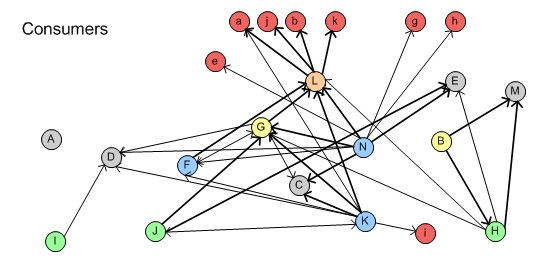
\includegraphics[scale=0.8]{consumers}
\caption{\label{fig:Consumers}IBM Study: Information consumers network}
\end{figure}

\begin{figure}[tbp]
\centering
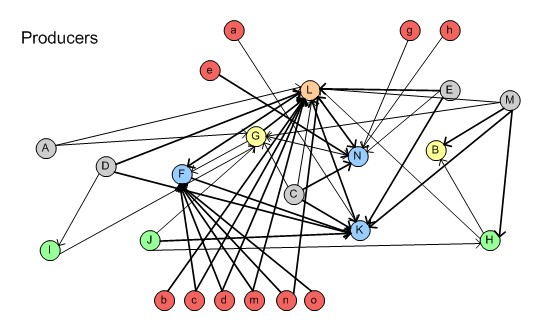
\includegraphics[scale=1.0]{producers}
\caption{\label{fig:Producers}IBM Study: Information producers network}
\end{figure}

Figure \ref{fig:Consumers} corresponds to the consumers' network. It represents, according to each node in the graph, who consumes the information produced by that person. Figure \ref{fig:Producers} corresponds to the producers' network. It represents (again, according to each node/person) who produces the information consumed by each person in the team. If all perceptions were equal, and if we had information from all relevant stakeholders, the second network should be equivalent to the first.

Figure \ref{fig:Mixed} mixes the first two networks, to obtain an information exchange network. It should be noted that the red (darker) nodes in the bottom, which correspond to technical groups and people, produce information that the project management team consumes, and this team then produces information that the red nodes in the top (business groups and people) consume. This was an unexpected pattern - as stated above, information flow in this team was supposed to be bidirectional between business and technical groups, not to flow mostly from technical to business people.


\begin{figure}[tbp]
\centering
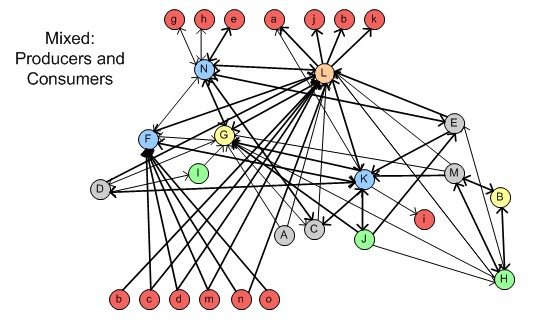
\includegraphics[scale=1.0]{mixed}
\caption{\label{fig:Mixed}IBM Study: Merged consumers and producers network}
\end{figure}

When we analyzed this pattern in greater detail, we found that people in the project management team do in fact communicate information from the business to the technical teams, but mostly at the start of a release cycle. The frequency and relevance of these communications are low. We believe this pattern might be a symptom of a disconnect between user needs and developer perceptions, which merits a closer analysis. This symptom is compounded by the following finding.

\textbf{Abstracted definition of success.} Almost all members of the project management team described their success criteria as shipping releases on time, with the expected features and the expected level of quality. However, nobody described success in terms of user satisfaction, or of meeting client expectations. The functional definition of success used by the team abstracts those considerations away.

This is problematic, since user needs and user requests go through close to a dozen ``hops'' until they reach the developers in charge of implementing them. If relevant information about satisfaction criteria or the intentions behind a requirement is dropped along the way, developers have no means to determine what it is that clients truly want.

We expected to find the project management team performing a ``client representative'' role in its interactions with the developers, but our data do not support this pattern. The ``client representative'' role may be performed by other teams in the division, but our data do not indicate whether these other teams do in fact communicate user concerns to developers, or if they rely on the release team to do so.

\textbf{Role specialization.} A few years ago, this project management team started to define its roles in greater detail, and to specialize its members. Today, the team seems to have a strong sense of the types of activities and responsibilities of each role. We have two types of evidence supporting this finding.

First, we asked every participant to sketch the structure of their team. In almost every case (except for the most recent additions to the team), the internal team structure was consistently well understood, even though few participants seem to have a strong picture of the relationship between the release team and the rest of the software division.

Second, the collaboration network of the team (shown in figure \ref{fig:Collaborators}) suggests a few very close collaborations as expected by those participants' roles, and a few weaker collaborations to other team members. Furthermore, comparing this network to the information exchange network (displayed above) shows that, although members collaborate with only a few people, they depend on many more to produce information essential for their activities. We believe this is an indication of a mature collaboration system in place.

\begin{figure}[tbp]
\centering
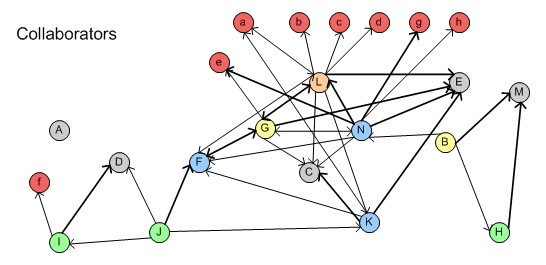
\includegraphics[scale=1.0]{collaborators}
\caption{\label{fig:Collaborators}IBM Study: Collaborators network}
\end{figure}

\textbf{Under-recognized role of interns.} Interns seem to do important (though perhaps routine) tasks, and to obtain as good a perception of the team dynamics as the managers in the team if they spend enough time working in it. Recruitment of interns for permanent positions might speed up considerably the learning curve involved in understanding the interactions and operations of a human system as complex as a software division. However, interns are rarely mentioned by other team members, and their mentorship is very informal. Based on our findings, we believe that a closer attention to the role and relevance of interns will be beneficial to the long-term efficiency of the project management team.

The findings reported above are, necessarily, an incomplete picture, since we restricted our analysis to a small team within a very large software division. A large scale study of the full division should yield insights with a much greater impact for its operation.

The study demonstrated the benefits of paying attention to the social and structural aspects of large-scale software development, but it also displayed the limitations of maintaining a narrow view of these phenomena. Although social and structural elements are major factors of software development and are worthy of consideration, the partial view they provided us with needed to be complemented with information about processes, physical location of team members, and the other perspectives described above. The proposal delineated in this appendix is the result of incorporating those ``missing perspectives'' into the study of shared understanding of software teams.


\chapter{Details of the Microsoft study}
\label{app:Microsoft}

In section \ref{sec:Microsoft} I present some information of the Microsoft study. We published these findings in the proceedings of the 2009 International Conference on Software Engineering \cite{Aranda2009}. The following text is an adaptation of fragments of that paper, included here for completeness.


\section{Motivation}

Modern large-scale software development demands managing huge quantities of bugs on a daily basis. Fixing them is one of the most common and time consuming activities of developers. When bugs number in the thousands, it is unfeasible for both team members and researchers to keep their details present in their minds. Abstraction becomes necessary: project health is measured by bug counts, for instance, and productivity by the rate of bugs closed.

Amid such abstractions it is easy to forget that every bug has a story behind it. The people that discover and resolve it need to coordinate, to get information from documents, tools, or other people, and to navigate through issues of accountability, ownership, and organizational structure. There are awareness requirements, inefficiencies, and opportunities for improved productivity and quality at every step in the process, yet these only become apparent when we go beyond the abstracted numbers and into the rich, detailed history of coordination in each bug.

As researchers, we often rely on repositories of software project information as the main or only source of evidence to extract the histories of bugs and other work items. They are usually stored in the form of tickets or records in a bug database. They provide a convenient compartmentalization of work. We use project management systems' features such as audit trails and data fields that keep track of ownership and of the context of each work item. Sometimes we enrich the histories in ticketing systems with records of electronic communication among team members, and with organizational structure data extracted from human resources databases. However, to this point the use of these electronic repositories as reliable and sufficient accounts of the history of bugs or work items has not been properly validated, and we do not have a description of the common coordination dynamics underlying bug histories.

Our paper reports on a field study of coordination activities around bug fixing that used a combination of case study research and a survey of software professionals. The study goes beyond the electronic repositories of software activity by talking directly to the key actors on the bugs to discover the patterns of group work that are commonly used to fix bugs. It discusses the reliability of electronic repositories as the basis of research into the coordination of software projects, and provides some implications for the design of coordination and awareness tools.


\section{Design and execution}
\label{sec:MicrosoftDesign}

The goal of our study was to provide a rich, contextualized, work-item-centric account of coordination in bug fixing tasks. We had two main research questions:

First, how is the process of fixing bugs coordinated in software teams? What is the lifecycle of bugs? What are the most common patterns of coordination involved in this work? How does their resolution play out over time and over the socio-technical network of the teams that work on them? Second, do electronic traces of interaction provide a good enough picture of coordination, or is non-persistent knowledge necessary to understand the story of each bug fix?

We executed a field study in two parts. The first was a multiple-case exploratory case study of bug histories. The second aimed to validate our case study findings with a survey of software professionals (developers, testers, and program managers). In both cases our data comes from software development at Microsoft's product divisions.

The unit of analysis of our case study was the history of a closed bug. We defined it as the collection of conceptually related activities that at some point in the life of their project were summarized as at least one entry in a bug database. Some records in bug databases are not bugs in the strict sense; we still treated them as such since our teams did. Some bugs have duplicate records; we considered all of the duplicates as part of the same conceptual entity. Some bugs exhibit symptoms that are initially seen as different bugs and recorded separately; we treated them as part of the same defect whenever possible. Bugs do not necessarily begin their life when the entry is created in the bug database or end when they are marked as ``Closed.'' Some of them extend further in both directions; this extended life is part of our unit of analysis. We selected our cases from three major product divisions at Microsoft. Our selection criteria were:

\begin{itemize}
\item The bug was filed in a bug database, and some elementary information about its nature was posted in its data fields.

\item The bug was marked as ``Closed'' at the start of our observations.

\item The bug was fresh (it was closed within two weeks of the start of our observations).
\end{itemize}

Our cases were selected randomly. Other data, such as the bug's resolution mechanism, were not part of our selection criteria, and we did not control for them. To get a better picture of the path that user-reported bugs follow, we deviated from our selection criteria in one case: we contacted a Customer Support escalation engineer and requested a pointer to a bug that had come from Microsoft's escalation channels (that is, a bug that was reported by a customer to support staff).

All of our cases followed the same methodology. First, we queried a product division's bug database to find a case fulfilling our criteria. We obtained as much information as we could from its electronic records, including the events in its audit trail, all the bug record's data fields, data on its owners and on everybody that had participated in any action related to the bug, and links to source code repositories. From that point, we traced backwards by contacting the people that had last touched or were referenced by the bug record. If they were not relevant to the history (a common case, due to bulk edits of bugs), we kept tracing back to find agents that were relevant for the bug.

Once found, we interviewed them to get their understanding of the history of the bug and of the participants and artifacts from which they obtained information or with which they coordinated to close it. When we were pointed to an artifact, such as a specification document, we analyzed it and traced back to its creators. When we were pointed to other people, we contacted them if possible, and repeated the process with them. When we were pointed to a persistent communication medium, such as an email, we obtained a copy, analyzed it, and traced back to its originators.

In some cases this process would reach a dead end but we knew there was more information to be found (because, for instance, we had yet to reach the point where the bug had been originally discovered). If that was the case, we jumped to the next relevant participant in the bug record and continued reconstructing the bug history from that point. We always made sure to reach the beginning of the story.

In other cases our inquiries would lead us to people and artifacts so far along the chain of events that they had little or no relevance to our bug's history. In those cases we made a subjective judgment call and stopped exploring those branches.

Our methodology was theoretically inspired in the focus on people, artifacts, and information flow of Hutchins' \shortcite{Hutchins1995} Distributed Cognition framework. However, as we had expected \cite{Aranda2006}, we found so many instances of information flow that executing our case studies at the computational and representational level of Hutchins' studies was not feasible. We tried to strike a balance between richness and contextual detail on one hand, and replication and generalization power on the other. We stopped collecting data on a chain of events when we had reconstructed it in full, or when we had reconstructed it partially, but proceeding further was unfeasible due to a lack of participation from some of its actors or due to our time constraints.

Our data collection was semi-structured. For each case we collected the following information:

\begin{itemize}
\item A list of primary and secondary actors in the history and their contributions.

\item A list of relevant artifacts and tools.

\item A chronological list of the information flow and coordination events in the bug's history.

\item Pieces of evidence as required by the particularities of each case.

\item The history of the bug as reconstructed by its record in the bug database.

\item The history of the bug as reconstructed by the full collection of electronic traces we obtained.

\item The history of the bug as reconstructed from making sense of all available evidence, including our interviews with participants.
\end{itemize}

In total, we studied ten bugs (including the escalation case). We interviewed 26 people. A brief summary of our cases is provided in table \ref{tab:MicrosoftCases}. Direct Agents are those who executed tasks in the process of resolving the bug; Indirect Agents were addressed by Direct Agents, but did not intervene.

We validated our case study results with a 54-question survey of software professionals at Microsoft. We sent it to 1,500 randomly selected Microsoft employees divided evenly between developers, testers, and program managers. We offered participants a chance to win a \$500US gift card. We received 110 responses (7.3\% response rate); all responses were optional but for all questions we received at least 100 responses. We did not control for the product division of the respondents or for demographic criteria.

The survey asked each respondent about the history of the last recently closed bug that they had played a primary role in resolving. It asked them to go over the corresponding record in the bug database and to bring up and re-read any emails pertaining to the bug, so as to have the history of the bug fresh in their minds.

The survey had three main parts. In the first, respondents gave us general data about the bug in question. In the second we questioned about coordination patterns. In the third, we probed the extent to which the record in the bug database told the full story of their bug.

Results from some of the general data questions appear in Figures \ref{fig:HowFound}, \ref{fig:KindBug}, and \ref{fig:HowClosed}. Although it is not appropriate to compare the case studies with the survey responses using statistical means, the two are mostly in agreement, with one exception: the number of direct agents identified in the case studies versus those reported in the survey. The quartiles for directly involved agents in the survey are 3 (25\%), 4 (50\%), 6 (75\%) and 15 (100\%). In contrast, three of our ten cases had more than 15 directly involved agents. We believe the difference suggests that our investigation revealed a much bigger bug footprint than our respondents perceive.


\begin{figure}[tbp]
\centering
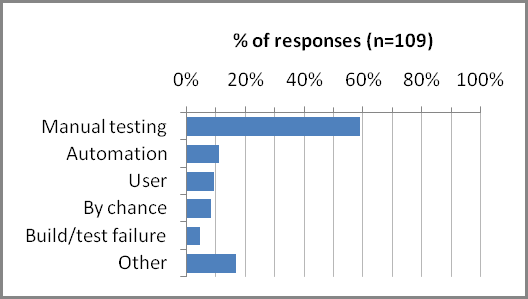
\includegraphics[scale=0.6]{howfound}
\caption{\label{fig:HowFound}Microsoft Study: How was this bug found?}
\end{figure}

\begin{figure}[tbp]
\centering
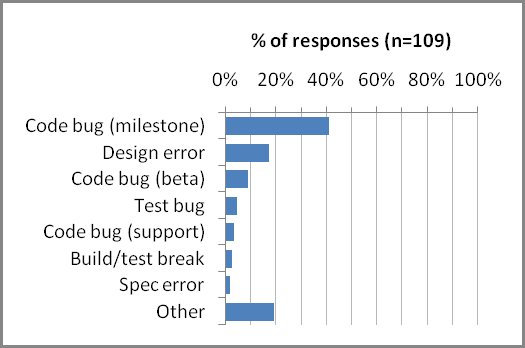
\includegraphics[scale=0.6]{kindbug}
\caption{\label{fig:KindBug}Microsoft Study: Kind of bug}
\end{figure}

\begin{figure}[tbp]
\centering
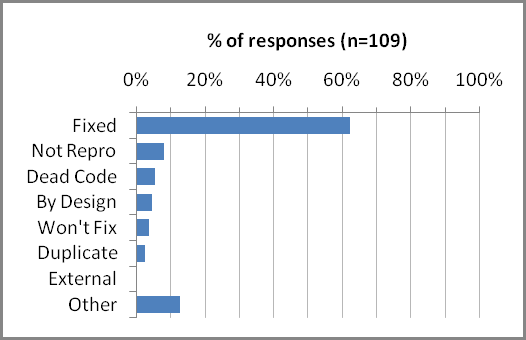
\includegraphics[scale=0.6]{howclosed}
\caption{\label{fig:HowClosed}Microsoft Study: How was this bug closed?}
\end{figure}


\section{Results and observations}

\subsection{Errors and omissions}

The most striking lesson from our cases is the deep unreliability of electronic traces, and particularly of the bug records, which were erroneous or misleading in seven of our ten cases, and incomplete and insufficient in every case. In fact, even considering all of the electronic traces of a bug that we could find (repositories, email conversations, meeting requests, specifications, document revisions, and organizational structure records), in every case but one the histories omitted important details about the bug. Before discussing the errors and omissions in these cases, we need to note that we believe this problem is not a consequence of a carelessness or lack of discipline particular to Microsoft. The repositories and documents we reviewed seem to be as thorough as those of comparable companies, or more.

We found there are several levels at which one can investigate the history of bugs, roughly corresponding to the amount of time one needs to invest in each of them. Each level incorporates all of the information acquired in the previous, plus additional findings from a deeper analysis:

\textbf{Level 1: Automated analysis of bug record data.} At the first level, one can use automation to obtain a list of agents that were involved in a bug's history, as well as information such as a bug's lifespan, its resolution, its changes of state, how was it found, who were its owners, which code change-sets correspond to the bug, and a chronological list of its events.

\textbf{Level 2: Automated analysis of electronic conversations and other repositories.} Traces of electronic conversations can be used to construct a social network of electronic interaction, and assume that it corresponds in structure and intensity to the real communication events of the participants. These data can be filtered by participants, keywords and timestamps to locate the electronic interactions that are (probably) related to the bug in question.

\textbf{Level 3: Human sense-making.} Automation is still far short of a human's capability to infer every connection in the data and reason about the evidence. First, there is often a wealth of information in the electronic repositories described above, but it is not formally linked�discovering it requires a semantic, unstructured analysis of the evidence. For instance, a note by person A in a bug record could state that a fix ``will not address group X's performance concerns, which will be filed in a separate bug.'' An adequately motivated human could conclude that there probably was a discussion between A and representatives of X, extract the list of people that are part of group X from a different database, match it with email records to identify the relevant conversation and agents involved, and, through trial-and-error queries (since no bug ID is provided), locate the follow-up bug in the database. Second, and posing an even greater challenge for automation, if we want to understand and improve coordination dynamics we need our bug histories to include the social, political, and otherwise tacit information that is also part of the bread and butter of software development. This is often subtle, not always apparent, and it must be read between the lines of the evidence collected.

\textbf{Level 4: Direct accounts of the history by its participants.} Interviewing the participants of a bug history seems to be the best gateway to obtain the information that was not documented, or it is disconnected, or erroneous. Interviews enrich significantly the data of the previous levels, as long as they take place before the history of the bug is forgotten. Although they are not guaranteed to provide us a complete account of the bug's history, they allow us to validate earlier conclusions, and to detect events that are not stored in the records, but that are essential to understand it.

We conducted our case study at the last of the four levels we listed. However, throughout its execution, we kept parallel bug histories corresponding to every previous level of analysis of the evidence, in an effort to determine how much of the real histories of bugs is gained or corrected at each level.

The differences between levels were stark, quantitatively and qualitatively. Tables \ref{tab:MicrosoftEvents} and \ref{tab:MicrosoftAgents} help to contrast them. Table \ref{tab:MicrosoftEvents} shows the number of events we could log, for each level, in the bug histories. Similarly, Table \ref{tab:MicrosoftAgents} shows the total number of agents (direct and indirect) found at each level.

Although the numbers support our claims, they cannot show the extent to which the bug histories diverge among levels. It is not just that higher levels produce longer stories; rather, they change qualitatively in ways that are deeply relevant to the study of coordination. The following paragraphs describe the most important kinds of divergence that we observed.

\textbf{Erroneous data fields.} Basic data fields in bug records were sometimes incorrect. C9 was a Test bug, but it was marked as a Code bug. Some duplicates of C2 and of C4 had the wrong Status (they were still marked as ``Resolved'' when their duplicates had been marked as ``Closed''). C8 was resolved as ``Won�t Fix,'' when it should have been resolved ``By Design.''

Our survey asked participants regarding about the Resolution field of their bugs, and their responses support our finding. 10\% of the respondents stated that the Resolution field of their bug was inaccurate.

\textbf{Missing data in bug record.} Among the important bits of data missing from bug records were links to the source code repository in C7 and C10, links to duplicate and related records of bug C2, links to a bug that was found in the process of resolving the original in C9, any links to specification documents (especially for case C5, resolved By Design), reproduction steps (C3), a statement of the corrective actions taken to fix the bug (C2, C4, C7), and a statement of the root cause of the bug (C7, C9).

The missing link to source code change-sets is one of the most problematic omissions. For the last bug of 70\% of our survey respondents, the fix involved committing code to a repository. But 23\% of those cases had no link from the bug record to the source.

The survey supports the rest of our findings too. Reproduction steps were marked as incomplete, inaccurate, or missing, 18\% of the time. Corresponding percentages for the root cause of bugs and the corrective actions taken are 26\% and 35\%.

\textbf{People.} Obtaining the lists of primary and secondary participants in a bug's history was a constant source of errors and omissions. People that took actions concerning the bug were often not mentioned in the record or in email communications (C2, C3, C7, C9, C10). The purported owners of a bug sometimes had no activities or stake in its resolution (C6, C7, C8, C9). The extent of a participant's contribution was easy to misjudge based on electronic traces: high frequency and intensity of interaction did not imply high level of contribution. And in at least two occasions, the geographic location of our interviewees was incorrect in the employee database.

In the survey, the people marked as ``owners'' of the bug were driving its resolution only in 34\% of the time. In 11\% they had nothing to do with the bug.

Furthermore, according to our responses, in 10\% of the time the primary people that worked on a bug are not easy to spot by looking at the bug record, and in 10\% they do not even appear in the record. The list of people that edited the bug's fields and history includes only some of its primary participants 40\% of the time, and none of them 4\%. Corresponding numbers for secondary participants are 39\% and 38\%. All of the people in the bug's history and fields are fully irrelevant in 7\% of the cases.

\textbf{Events.} It is unrealistic to expect all events related to a bug to be found in its record or through its electronic traces. Naturally, most face-to-face events left no trace in any repository. But in some occasions, the key events in the story of a bug had left no electronic trace; the only way to discover them was through interviews with the participants. At the same time, some events logged in the bug records of all of our cases were noise or junk (for instance, bulk edits and mistakes with their later corrections). The chronological order of events was also problematic: bugs were sometimes resolved even before their record had been created (C7), or closed long after they had been resolved because they had been forgotten by the person that needed to close them (C2, C4).

In the survey, 3\% of the bugs had been discussed at least a month before they were first filed, and an additional 6\% at least a week before being filed.

\textbf{Groups and politics.} As we moved further from the raw data and into broader patterns of coordination, we saw that most of the important information at the team and division levels could only be found through higher levels of analysis. In C4 we found a pocket of people with a culture and practices different than those of their division, in the process of assimilation after an acquisition. The status of a group with respect to milestones and releases bore significant consequences to the kind and speed of the decisions made as new bugs were found (for instance, for C5 the team was undergoing a ``bug bash'' and having face-to-face triage meetings daily; most bugs were only given a minute of air time or less). Sometimes, as in C3 and C7, ownership of a bug falls in a gray zone, and inter-team or inter-division struggles to determine ownership and accountability ensue. These issues usually impact the history of bugs considerably, yet we could not have learned about them without interviewing its participants and paying close attention to the details in the electronic record.

\textbf{Rationale.} Probably the hardest questions to answer without human sense-making and participant collaboration were the ``why'' questions: in C4, why did a developer choose another as a required code reviewer, but a third as an optional reviewer? In C10, why was there no activity in a bug record for weeks after a few bouts of minute-by-minute updates and frantic emails? Why were the Status or Resolution fields in C2, C4, and C8 incorrect? Why in C5 did a triage group conclude that the bug would not be fixed? Why did a tester file a bug, C9, even though she suspected the failure was most likely a false alarm? We found that the answers to these questions, discovered during interviews, would often unlock the whole explanation of the events in the history of a bug.

\textbf{Miscellaneous.} Other facts that could only be found at higher levels of analysis resist categorization, but still tend to be at the heart of a bug's history. In C6, a bug was found independently by a tester and a developer in different groups; the developer produced a fix without knowledge that the bug had been already documented. In C4, a developer committed hundreds of new lines of code to fix a bug shortly after it was found; he did not write them all at a blazing speed, but rather copied them from the code of his old company, now acquired by Microsoft, and ``stitched it'' to the relevant interfaces. In two cases (C3 and C7), early and correct diagnoses were promptly ignored in a flurry of emails to get an urgent bug resolved. In general, the bugs in our case pool had far richer and more complex stories than would appear by automatically collecting and analyzing their electronic traces.

\subsection{Coordination Patterns}

In the end, our bug histories were rich, varied, and context dependent. They did not follow a uniform path or lifecycle. This posed a problem: our first research goal was, precisely, to describe the lifecycle of bugs and the process of fixing them.

Instead of attempting to formulate a process for all bug histories, we chose to describe the menu of coordination patterns that we observed. We selected the patterns that seemed to be the most recurrent and those that occurred rarely but had a great impact in the history of a bug. Tables \ref{tab:MicrosoftPatterns1} and \ref{tab:MicrosoftPatterns2} list them.

Some of the patterns have negative implications. For instance, we saw several cases of ``snowballing threads'' and ``rapid fire email in public'' that were clearly inefficient, yet they seemed to be routine for our participants. The only ``summit'' we observed corresponded to a bug (C3) that was described to us as ``very important'' and ``threatening to move our ship date'' by the release manager in charge. We added one pattern for completeness (video conferences), though we observed no instances of it. Another pattern, ``forgotten,'' was pointed to us by one of our survey respondents; it was not included in our original list.

We asked our survey respondents whether those patterns had occurred for their last bug, and if so, whether they had been essential for the resolution of the bug. Figure \ref{fig:Frequencies} provides their responses. The last column represents the perceived usefulness of a pattern in relation to its frequency.

\begin{figure}[tbp]
\centering
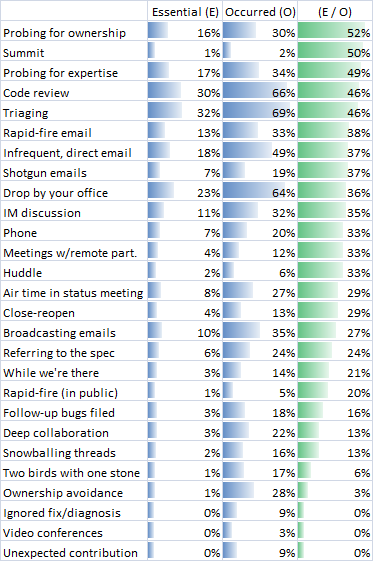
\includegraphics[scale=0.8]{frequencies}
\caption{\label{fig:Frequencies}Microsoft Study: Coordination pattern frequencies}
\end{figure}

We do not claim that our list of patterns is comprehensive. But using them to characterize bug histories may provide enough relevant information about their coordination events while ignoring irrelevant details. Furthermore, some of them could be supported (or in the case of negative patterns, prevented) by software tools.

Although the set of states commonly used in bug databases (Active, Assigned, Resolved, etc.) may be helpful to manage software development, our data shows that they are poor approximations of the true lifecycle of a bug. We believe it is more useful, for understanding coordination and for designing tools for developers, to think of bug fixing activities not as belonging to a stage of a bug�s life or a workflow, but as striving for the satisfaction of one or several goals.

We formulated a list of goals based on the activities of the people in our case study. The following paragraphs describe them. Not all of the goals occur for every case, and they do not occur strictly sequentially.

\begin{itemize}
\item \textbf{Discovery.} Detecting a difference between reality and expectation. The essential first step to record the unexpected behavior as a bug.

\item \textbf{Diagnosis.} Understanding the nature, cause, and impact of the bug, as well as the actions that will be taken as a result. We believe it happens in every case, though often tacitly.

\item \textbf{Assignment of Ownership.} Determining who will be responsible and accountable for the resolution of a bug, both at the group and individual levels.

\item \textbf{Search.} Finding the appropriate knowledge, resources, and skills. It seems to be often meshed with Assignment of Ownership activities, so that the expert is the owner of the bug �but even the owner may need to reach out for other, more specific bits of expertise and knowledge.

\item \textbf{Correction.} What we usually think of as ``fixing a bug.'' Correcting relevant lines of code, changing documentation, scripts, or other artifacts so that reality and expectation match again.

\item \textbf{Closure.} Determining that the organization is willing to live with the current state of things as related to the bug.

\item \textbf{Awareness.} Communicating status to relevant participants. It stretches through the whole history of almost every bug.
\end{itemize}

These goals provide a framework to analyze the effectiveness of coordination and project management tools and practices. For instance, \emph{Assignment of Ownership} is often problematic, especially if there is no clear owner of the seemingly buggy code. In the case study this happened more often with test scripts than with feature code, and with developers leaving their posts without tying loose ends. Tools and practices that ensure that every artifact has an active owner would reduce this problem.

\emph{Search} is another problematic area. In our cases it often resulted in ``snowballing threads'' and ``shotgun emails,'' which sometimes succeed in finding the people or piece of knowledge necessary, but can be extremely inefficient if one considers the person-hours needed by hundreds of email recipients to parse numerous messages that, more often than not, have no relevance for them.

For coordination purposes, \emph{Awareness} was the area most in need of improvement. However, it is not easy to figure out how to provide the right level of awareness in very large companies with interconnected products. Awareness seems to be most needed not at the team level, but among the primary and secondary agents that form the social network around a work item. Tools that (partially) detect work networks and allow for their members to be aware of the activities of their peers should help address this issue.


\section{Limitations}

During our analysis we worked with several concepts that do not yet have a consistent definition in the literature. In particular, one could argue that our coordination patterns and goals are subjective and have blurry boundaries�we never specified, for instance, the difference between ``rapid-fire'' and ``infrequent'' emails. Although this is a valid criticism, our constructs are a first iteration given the data we collected. Additional data and further iterations should refine these constructs, and add others that help convey the underlying concepts more clearly.

Our data come exclusively from Microsoft, and the extent to which our results are valid for other companies is not clear without replications. As is well known, Microsoft has tens of thousands of employees, millions of daily users, and many interconnected products. These are all forces that shape coordination dynamics. However, the use of software repositories and communication media at Microsoft seems to be similar to that of comparable companies. The clearest finding in our study, the difference between the minable version and the true version of a bug's history, should not be Microsoft-specific, as it depends not on corporate culture but on the amount and quality of the information that can be economically and efficiently captured electronically. It is possible that for some software development environments, particularly open source, in which all or most information is communicated electronically and persistently, this is less of a problem. Replications of this study would help resolve that question.
\chapter{Details of the Contrast study}
\label{app:Contrast}

Most of the studies on which this thesis is based have been peer-reviewed and published. The exception is the \emph{Contrast} study, for which no publication yet exists. The reason is that I concluded my data collection for that study only recently, and writing this thesis has been more pressing than publishing the results of the study. However, in the interest of providing some context for the findings from the Contrast study discussed throughout the thesis, I offer some of the details of the design and execution of the study in this appendix.

\section{Motivation}

Our ``Requirements in the Wild'' paper \cite{Aranda2007} offered two competing hypotheses to explain the variability in project management practices in our cases. The first stated that the diversity of processes and practices in small firms can be explained as the result of evolutionary adaptation, as these firms have adapted to a specific niche. The second, in comparison, claimed that the choice of processes and practices is irrelevant for small firms with strong cultural cohesion, as the efficiency of team dynamics overrides any benefits based on process. For the first, the choice of processes and practices was an essential strategy for the survival of the firm; for the second they were accidental habits that might as well have been different had the organization members wished so.

Thanks to Greg Wilson, we identified two organizations in which we could execute a comparative case study to evaluate these hypotheses. The organizations seemed to be ideal for a comparison for a variety of reasons. First, at the time we selected them, they had similar sizes (about 90 people). Second, both of them were well established, having been active for several years. Third, they serviced similar kinds of organizations; in particular, both organizations had clients in the health, insurance, and financial sectors. Fourth, and most importantly, the organizations had purportedly very different approaches to develop software.

We knew from our requirements paper that Bespoker had a relatively formal, process- and document-heavy approach to software development. We were not sure, however, to what extent these processes and documents were an essential part of of the strategy of the organization, that is, to what extent they were incorporated in decision-making, and in coordination and communication, and to what extent they were formalities produced out of habit, convenience, or customer requests.

In comparison, the second firm, which here we called Saville, was an advocate of Extreme Programming, something that was rather unusual given its moderate size. A tour of the organization confirmed, at least on a surface level, Saville's commitment to the Agile Manifesto: all projects were developed in team rooms, pair programming and story cards were commonplace, and customer representatives were present at all times to answer questions to developers.

It seemed, then, that we had found two organizations with very similar contexts and very different software development strategies. This appeared to be a challenge to the first hypothesis and a confirmation of the second. Our motivation, therefore, was to probe this seeming support for the latter hypothesis, and to evaluate whether the differences were truly deep or superficial. The study eventually led to other, I believe more important, insights about coordination and communication in software development. But this was our initial reason to execute the study.



\section{Design and execution}
\label{sec:ContrastDesign}

Our research questions called for a comparative case study of Bespoker and Saville. The unit of analysis was the organization itself.

In both organizations I negotiated full access to the offices for three weeks. I visited Saville during the Summer and Bespoker during the Fall of 2009. During the three weeks that I spent at each site I attended meetings, performed fly-on-the-wall observations of developers at work, and interviewed roughly half of the members of the organization. For both organizations there were a few key people that I could not interview during my three-weeks period; I returned to the organizations when their schedules allowed me to get those interviews.

At Saville I spent two weeks in its headquarters office and one week in the satellite office. I spent at least one day, but often more, sitting in each of the firm's team rooms, in any empty spot I could find. At Bespoker I was assigned a desk in one of the project areas. The strategy I used at Saville (to sit with the teams and informally interview anyone that seemed to be available at any given moment) did not work well at Bespoker, and during my first week at Bespoker I did not get much information: there was very little interaction happening verbally, and everyone would mostly work silently facing their computers most of the day, except during lunch time (and for some people, even during lunch time). Most of the visible verbal interaction was \emph{sotto voce}. So I resorted to scheduling brief interviews with members of the organization, which worked much better, as most people were happy to give some time to this study.

As a result of my observations and interviews I wrote about two hundred pages of detailed notes, and I collected copies of some documents from both sites that I considered important or meaningful in some ways. I coded these qualitative data, iterating on my list of codes until I felt that the salient aspects of the notes were being properly considered.

Although I endeavoured to remain objective, open, and impartial, the fact that I alone performed all data collection and analysis for this study may have introduced some biases in its findings. However, it also enabled me to gain the trust of many members of the organization, and to perform a thorough and cohesive analysis of the data.

After I finished my observations, I applied a social networks survey to members of both organizations. The survey had the form of a spreadsheet, with seven questions to be answered for each member of the organization, so that Person A would answer each question for persons B to Z. To simplify the task of responding over 600 questions, the spreadsheet had a default, expected answer for each of them, and the respondent would simply need to change the answer for those questions he or she deemed necessary. One of my contacts at Saville tested the survey and suggested many improvements for clarity and for ease of responding. Specifically, the questions were the following:

\begin{itemize}
\item Write a 1 next to every person that you manage directly.

\item Write a 1 next to every person that manages you directly.

\item Write a 1 next to every name of people you wouldn't recognize.

\item Professionally, how much do you interact with this person? (0=not at all, 1=a little, 2=lots)

\item Personally, how much do you interact with this person? (0=not at all, 1=a little, 2=lots)

\item How much do you depend on information from this person? (0=not at all,      1=a little, 2=lots)

\item How much does this person depend on information from you? (0=not at all, 1=a little, 2=lots)

\end{itemize}

I had permission to send the survey to the full list of staff of Bespoker and to a randomly selected half of the staff at Saville. At Bespoker, 19 out of 47 people responded, or 40\% of the total. At Saville, 23 out of 43 people in the sample (and out of 90 people in the full organization) responded, or 53\% of the sample (and 26\% of the population). The respondents were evenly distributed between working teams in both organizations, but at Bespoker there was a higher rate of manager responses. As I describe in section \ref{sec:NetworkDensity}, this survey response bias appeared to affect some density figures. I wrote Python scripts to extract density results from these responses.



\section{Details of the firms}

\subsection{Saville}

Saville is a 90-person software development firm founded in 1990. It now services a variety of industries, including health, insurance, finance, and the government. It has three major project divisions, each with about 25 people, although the number of people in each division changes depending on project demands. Saville has two offices in the Toronto area, both easily reachable through public transit, and all of its software development occurs in these offices. The headquarters are the larger office; two of the three divisions are located in the headquarters. Until recently all three divisions were located there, but space problems led the firm to rent another location and move one of its divisions there.

Each division has a small number of team rooms, where all of the developers sit. In most teams developers do not have a permanent spot or desk. They have a locker where they can store their personal belongings, but they are expected to move around rooms (and within rooms) as necessary. This is less true at the satellite office, where there is an informal understanding that a seat is claimed by somebody in particular, even though at any given moment that person may be working at someone else's seat.

Saville is an advocate of Extreme Programming and Lean Manufacturing techniques. It is involved in the Toronto Extreme Programming community, and has an office staffed by two persons dedicated to ensure that the processes, practices, and tools of all teams are consistent with the culture of the organization, and with helping all teams with coaching, training, and technical infrastructure issues.

The organization did not start as an agile shop. In fact, the Agile movement did not exist as such when the firm was founded. Its conversion occurred as a result of the interest in Extreme Programming by two of the senior developers of the organization and by the direct influence of Kent Beck, the main proponent of Extreme Programming, who had been a Smalltalk consultant for the organization years before.

However, I found that Saville was not simply an Extreme Programming firm: it would not do software development necessarily by the Extreme Programming book. Agile practices were common in some teams and infrequent in others. One of the divisions insisted in having all production code developed in pairs; another division would pair program only occasionally. All teams had a daily stand-up meeting, but while these meetings were highly informative in some teams, they were merely a formality in others. All teams used user stories and story cards to keep track of their requirements, but some also used more detailed documentation (usually because it was required by their customer), and one division employed two business analysts. Customer representatives were present in two of the three divisions. The picture that emerged was of a firm formed by three porous divisions with different (though generally high) levels of commitment to agile strategies and a careful control and reflection over its software practices and group formation.



\subsection{Bespoker}

Bespoker is a 43 person software development firm founded in 2001. At the time of our case selection it was a larger organization of nearly 90 people, but the firm was severely hit by the 2008-2009 recession and lost most of its contract staff before my observations began. Like Saville, it services the health, insurance, and finance industry. It also has data warehousing and web development projects.

Bespoker has a team-based structure: teams are formed for a project; each team usually has one project manager, and every project falls under the portfolio of one of the partners of the organization. Physically, the headquarters and only offices are located in one site in the Toronto area easily reachable through public transit. Most of the analysis and software development occurs in this site, although the firm sometimes uses desks in its customers' offices, specially those of a bank, when possible and convenient. Although the members of a team sit in the same area, their desks are arranged to balance proximity and isolation. There are no cubicles, but there is a sense that a desk and its surrounding area is a person's own. Perhaps as a consequence of this the environment is much more quiet than at Saville, where there is a constant buzz of activity in every team room. At Bespoker there is verbal communication happening during office hours, but people sometimes choose to communicate over instant messaging or e-mail, even when they are a few steps away from each other.

Software development at several teams in Bespoker usually follows a planned, iterative approach, with a discovery phase, several iterations, and deployment. In occasions iterations continue after deployment. The documents produced in the analysis section of each iteration can be quite thorough: one requirements document, for instance, was 83 pages long, and it had numerous UML diagrams of use cases, classes, and sequences. However, some projects, such as the outlying web development projects and the data warehousing one, do not seem to follow this structure, and even in teams that produce these documents there is often the sense that they are produced as deliverables or as artifacts of record, and they are not used intensely during development. Few of the developers I spoke to, for instance, claimed to read the specification before working on their next feature; they would rather talk to the analyst that produced the specification to figure out the purpose of their feature, and only use the document, on occasion, as a reference. Though the firm claims to be as agile as possible given its context, this does not seem to be the case.

Overall, the emerging picture of Bespoker is that of a firm with a mature homegrown process and set of practices, but little philosophical commitment to any software development strategy. It relies mostly on familiarity and habit, a strategy that has served it well over the years, but that is challenged by the firm's recent incursions in unfamiliar domains.


\section{Results and observations}

The following pages are intended to give a brief overview of some of the main findings from this study. Some of these findings also appear over the footnotes of Chapter \ref{chap:SharedUnd}, in the context in which they appear relevant to the discussion.

\subsection{Adaptation \emph{vs.} cohesion}
\label{sec:AdaptationVsCohesion}

The question of whether firms adapt their software development processes to suit their niches or rely instead on cultural cohesion to survive was the original motivation for this study. If the former is true, then selecting the right process is essential; if the latter, then processes are basically accidental characteristics of software firms. The implications of both answers are deeply relevant to our field; hence the interest in resolving the question.

Neither hypothesis is fully supported by our data. First, it is clear that both Bespoker and Saville have modified their development strategies over time. Saville underwent a considerable transformation roughly ten years after its foundation from a somewhat chaotic software house to a full-fledged, intentional Extreme Programming outfit. It has suffered other changes since then, but none at this level. Bespoker, in turn, has had to abandon (or at least downplay) its standard formalized process as it explores some unfamiliar domains, and it has incorporated more frequent iterations in its more traditional projects, partly in response to complaints that it is not ``agile enough.'' The move towards Extreme Programming at Saville does not appear to be based on demands of its niche---on the contrary, Saville has had to educate its customers and to manage their expectations, since its development strategies are atypical. In fact, several of Saville's minor changes have been an adjustment in the opposite direction: providing more structure and more formalization for the customers that request it. At Bespoker, some of the changes appear to be responses to the firm's context, or to inadequacies of its standard process in some domains. But if a team at Bespoker does not encounter strong obstacles to execute the strategies it is familiar with, then the team will simply use those strategies without much thought on optimizing them for their current situation. In other words, although part of the changes in both firms can be explained as adaptation to the demands of their niche, this adaptation is not judged essential to the survival of the firms, and in many cases the firms can impose the development strategy of their choice with only minor adaptations. The diversity of software development strategies does not seem to be dictated by organizational context.

Second, it is also clear that cultural cohesion, on its own, is not enough to guarantee success in software development. While cohesion is strong (see below in section \ref{sec:NetworkDensity}) and assiduously nurtured in both organizations, their members care deeply about their development strategies and do not feel as if all sensible strategies would work equally well for them. Saville employs an agile coach, and two members of its staff have the responsibility to oversee the firm's software development strategies. Bespoker managers attempt to have a relatively tight control over its strategies, and are uncomfortable in the domains where they have to relinquish some of this control. Therefore, although cohesion seems to be a very relevant characteristic of both firms, the claim that software development strategies are entirely accidental as long as the organization has a good degree of cohesion is not fully supported either.

An explanation for the variety of software strategies that is based exclusively on a combination of both hypotheses is also unsatisfactory. Through my observations at Bespoker and Saville I realized that a significant part of the behaviour of both firms cannot be fully explained as a combination of evolutionary adaptation and reliance on cohesion. Personal convictions, habits, preferences, professional abilities, and tactical decisions all seem to play a role in the behaviour of the members of these firms; these elements are not properly captured with a combined-hypotheses model.

The problem appears to arise from conflating several concepts in these hypotheses; concepts that should be kept separate due to their qualitative differences. The adaptation hypothesis merges project lifecycle processes, documentation, practices, and tools. Choices on some of these may be mandated by the organization's context, some may not. In turn, the cultural cohesion hypothesis merges preference, expertise and task familiarity with group cohesion proper; concepts that should be studied separately. This thesis articulates what I think is a more fitting framework for these concepts.


\subsection{``Spreading the knowledge''}
\label{sec:Spreading}

The most interesting findings from my observations at Saville and Bespoker were the organizations' efforts at coordinating and communicating efficiently. These efforts were more evident and intentional at Saville than at Bespoker, but they were a core concern of both firms.

Several members of Saville took an explicitly generalist approach to coordination and communication. They would refer to their efforts as ``spreading the knowledge,'' so that, for instance, pairs of programmers would often be selected on the basis of where and to whom did the team need to spread the knowledge of a component of their projects next. They talked about the need to avoid specialization (``silo culture''), and regretted the instances where specialization had taken a hold in the organization.

When a team would be ready for a new user story, a group of about five people would hear a small, informal presentation of the user story by one of the team members, and would discuss implementation possibilities and challenges. Throughout the meeting, the team would list the tasks that were necessary to complete the story; at the end they would estimate the effort necessary to complete the task for a pair of programmers, and they would discuss who would take over the development of the story.

Every morning, every team had a short ``stand-up meeting,'' in which the team members would discuss their previous day's activities and obstacles, and talk about possible activities for the day. Although in some teams this meeting had devolved to a rote and meaningless practice performed out of habit, in most others the meetings had clear benefits for the team members. 

Saville's efforts to coordinate and communicate relied intensely on synchronous, proximate, and proportionate team interaction, and less directly on maturity. The stand-up meetings, as well as the user story definition practice and the efforts to ``spread the knowledge'' are but three of the many strategies used by the firm, as discussed in Chapter \ref{chap:SharedUnd}.

In comparison, Bespoker had a less intentional aproach to ``spreading the knowledge.'' In fact, such knowledge was not visibly or audibly accessible most of the time: a silent observer such as myself could find very little about Bespoker's strategies without engaging with and interviewing the members of the organization. However, the firm has settled with several strategies to coordinate and communicate, strategies that are well-known to most members of the organization and that rely on formalization (for several projects) and direct face-to-face interactions with a few key people in a team (for other projects). When the firm enters into a new domain, or finds its context changing significantly in one of its older domains, as with the offshoring project, the struggles to coordinate and communicate are most evident.

However, overall, Bespoker's coordination and communication strategies rely mostly on maturity, and to a lesser extent on synchrony, proximity, and proportionality. This points to a potential for improvement, considering that the organization is almost entirely co-located, and could explore synchronous and proximate interaction strategies with relative ease.


\subsection{Network density}
\label{sec:NetworkDensity}

I extracted basic network density numbers from the survey at both sites. Table \ref{tab:NetworkDensity} presents the results. Note that for one question (``People you wouldn't recognize'') I inverted the direction of the question and of the answers, so it is now (``People you recognize'').

\begin{table}[tph]
\caption{\label{tab:NetworkDensity} Network densities of Bespoker and Saville}
\centering
\footnotesize{\begin{tabular}{p{5.6cm}p{4.0cm}p{4.0cm}}
\hline \hline
\vspace{1pt} \bfseries Network & \vspace{1pt} \bfseries Bespoker & \vspace{1pt} \bfseries Saville \\
\hline
\vspace{0.5pt} People you manage & \vspace{0.5pt} 7.09\% & \vspace{0.5pt} 1.45\% \\
\hline
\vspace{0.5pt} People that manage you & \vspace{0.5pt} 4.69\% & \vspace{0.5pt} 2.42\% \\
\hline
\vspace{0.5pt} People you recognize & \vspace{0.5pt} 92.33\% & \vspace{0.5pt} 88.70\% \\
\hline
\vspace{0.5pt} People you interact with professionally & \vspace{0.5pt} 44.97\% (at least a little); 15.90\% (lots) & \vspace{0.5pt} 47.49\% (at least a little); 19.08\% (lots) \\
\hline
\vspace{0.5pt} People you interact with personally & \vspace{0.5pt} 40.50\% (at least a little); 11.33\% (lots) & \vspace{0.5pt} 35.80\% (at least a little); 8.45\% (lots) \\
\hline
\vspace{0.5pt} People whose information you depend on & \vspace{0.5pt} 27.92\% (at least a little); 10.30\% (lots) & \vspace{0.5pt} 21.11\% (at least a little); 7.39\% (lots) \\
\hline
\vspace{0.5pt} People who depend on your information & \vspace{0.5pt} 26.32\% (at least a little); 8.01\% (lots) & \vspace{0.5pt} 22.37\% (at least a little); 8.60\% (lots) \\
\hline
\end{tabular}}
\end{table}

Some of these figurs require explanation or discussion. More managers responded to the survey at Bespoker than at Saville, which partially explains the differences in the first question; the other part of the explanation being the somewhat more pyramidal hierarchy at Bespoker. The number for  ``people you recognize'' at Bespoker, though higher than at Saville, is more alarming, considering that Bespoker has half the staff of Saville and that it has a single development site against Saville's two. Both firms, however, seem to be crossing a threshold where more and more of their peers will be strangers for them, should the firms keep increasing in size.

These basic network density numbers may be misleading, as both Bespoker and Saville have several teams where, presumably, workflow is far more intense than table \ref{tab:NetworkDensity} indicates. To explore this I performed an additional analysis of the density numbers, where I would only consider a participant's responses corresponding to the team the participant belongs to. For this second analysis I ignored responses from managers and support staff. The results are summarized in table \ref{tab:NetworkClusters}.

\begin{table}[tph]
\caption{\label{tab:NetworkClusters} Team-based network densities of Bespoker and Saville}
\centering
\footnotesize{\begin{tabular}{p{5.6cm}p{4.0cm}p{4.0cm}}
\hline \hline
\vspace{1pt} \bfseries Network & \vspace{1pt} \bfseries Bespoker & \vspace{1pt} \bfseries Saville \\
\hline
\vspace{0.5pt} People you manage & \vspace{0.5pt} 26.21\% & \vspace{0.5pt} 5.90\% \\
\hline
\vspace{0.5pt} People that manage you & \vspace{0.5pt} 11.62\% & \vspace{0.5pt} 6.55\% \\
\hline
\vspace{0.5pt} People you recognize & \vspace{0.5pt} 97.09\% & \vspace{0.5pt} 98.91\% \\
\hline
\vspace{0.5pt} People you interact with professionally & \vspace{0.5pt} 83.50\% (at least a little); 51.46\% (lots) & \vspace{0.5pt} 70.96\% (at least a little); 39.96\% (lots) \\
\hline
\vspace{0.5pt} People you interact with personally & \vspace{0.5pt} 59.22\% (at least a little); 20.39\% (lots) & \vspace{0.5pt} 41.48\% (at least a little); 12.23\% (lots) \\
\hline
\vspace{0.5pt} People whose information you depend on & \vspace{0.5pt} 53.40\% (at least a little); 22.33\% (lots) & \vspace{0.5pt} 41.27\% (at least a little); 22.05\% (lots) \\
\hline
\vspace{0.5pt} People who depend on your information & \vspace{0.5pt} 55.34\% (at least a little); 16.50\% (lots) & \vspace{0.5pt} 37.99\% (at least a little); 19.21\% (lots) \\
\hline
\end{tabular}}
\end{table}

Unsurprisingly, the density numbers are higher across the board. However, a note of caution in interpreting this table is necessary. For Saville there are three clusters, corresponding to its divisions. Bespoker does not have such an organizational structure; it creates teams on a project basis. Among the respondents I was able to use data for six of Bespoker's projects, some of them with very few participants. Naturally, then, information dependence and interaction were higher in the case of Bespoker. When analyzing these tables, the reader should remember that these basic density figures are meant to be analyzed as part of the larger body of collected data of the Contrast study, not as stand-alone descriptions of the two firms.


\end{document}
